\documentclass{beamer}
\usetheme{Dresden}
\usecolortheme{dolphin}
\usefonttheme[onlymath]{serif}

%\pdfminorversion=7 % per togliere il warning delle immagini

\setbeamertemplate{navigation symbols}{} %toglie i navigation symb. basso a dx
%\setbeamertemplate{mini frames}{} % boh non fa niente
\renewcommand*{\slideentry}[6]{} % toglie i pallini in alto
\setbeamertemplate{section in toc}[ball unnumbered] % mette i bullet nella toc

\usepackage[utf8]{inputenc}
\usepackage[T1]{fontenc}
\usepackage{lmodern}
\usepackage[british]{babel}
\usepackage{amsmath}
\usepackage{amsthm}
\usepackage{graphicx}
\usepackage{subfig} % affiancare figure
\usepackage{caption} % per gestire meglio le didascalie
\usepackage{pgfplots}
\pgfplotsset{compat=newest}
\pgfplotsset{plot coordinates/math parser=false}
\usepackage{booktabs} % per i filetti delle tabelle
%\usepackage{wrapfig} % a cosa mi serve?
\usepackage{appendixnumberbeamer} % numerare da 1 nell'appendice
\usepackage[separate-uncertainty=true]{siunitx} % per le unitàdi misura

\captionsetup{skip=0pt, belowskip=0pt}
\captionsetup{labelformat=empty}
\captionsetup[subfigure]{labelformat=empty}
%\captionsetup{singlelinecheck=false}
\setbeamerfont{caption}{size=\fontsize{5}{7}}
\pgfplotsset{every tick label/.append style={font=\tiny}}

\usecolortheme{orchid} % per i block
\setbeamercovered{transparent}

\newlength{\widthconslaw}\setlength{\widthconslaw}{0.9\textwidth}
\newlength{\heightconslaw}\setlength{\heightconslaw}{0.43\textheight}
\newlength{\limiterswidth}\setlength{\limiterswidth}{0.96\textwidth}
\newlength{\limitersheight}\setlength{\limitersheight}{0.65\textheight}
\newlength{\tvdwidth}\setlength{\tvdwidth}{0.9\textwidth}
\newlength{\tvdheight}\setlength{\tvdheight}{0.5\textheight}
\newlength{\figwidth}\setlength{\figwidth}{0.4\textwidth}
\newlength{\roughwidth}\setlength{\roughwidth}{0.9\textwidth}
\newlength{\roughheight}\setlength{\roughheight}{0.9\textheight}
\newlength{\bfswidth}\setlength{\bfswidth}{0.95\textwidth}
\newlength{\bfsheight}\setlength{\bfsheight}{0.8\textheight}
\newlength{\bfshalfwidth}\setlength{\bfshalfwidth}{0.5\textwidth}
\newlength{\cavheight}\setlength{\cavheight}{0.7\textheight}
\newlength{\timewidth}\setlength{\timewidth}{0.65\textwidth}
\newlength{\timeheight}\setlength{\timeheight}{0.65\textheight}
\newlength{\timehalfwidth}\setlength{\timehalfwidth}{0.45\textwidth}
\newlength{\timehalfheight}\setlength{\timehalfheight}{0.82\textheight}
\newlength{\widthsette}\setlength{\widthsette}{0.4\textwidth}

\graphicspath{{../img/}}

%%%%%%%%%%%%%%%%%%%
% per la numerazione delle slides
\newcommand{\frameofframes}{/}
\newcommand{\setframeofframes}[1]{\renewcommand{\frameofframes}{#1}}

\setframeofframes{of}
\makeatletter
\setbeamertemplate{footline}
{%
	\begin{beamercolorbox}[colsep=1.5pt]{upper separation line foot}
	\end{beamercolorbox}
	\begin{beamercolorbox}[ht=2.5ex,dp=1.125ex,%
		leftskip=.3cm,rightskip=.3cm plus1fil]{author in head/foot}%
		\leavevmode{\usebeamerfont{author in head/foot}\insertshortauthor}%
		\hfill%
		{\usebeamerfont{institute in head/foot}\usebeamercolor[fg]{institute in 
		head/foot}\insertshortinstitute}%
	\end{beamercolorbox}%
	\begin{beamercolorbox}[ht=2.5ex,dp=1.125ex,%
		leftskip=.3cm,rightskip=.3cm plus1fil]{title in head/foot}%
		{\usebeamerfont{title in head/foot}\insertshorttitle}%
		\hfill%
		{\usebeamerfont{frame number}\usebeamercolor[fg]{frame 
		number}\insertframenumber~\frameofframes~\inserttotalframenumber}
	\end{beamercolorbox}%
	\begin{beamercolorbox}[colsep=1.5pt]{lower separation line foot}
	\end{beamercolorbox}
}
\makeatother
%%%%%%%%%%%%%%%%%%%%%%%%%%%%%%%%%
\title{A fully implicit formulation for Navier-Stokes/Darcy coupling}
\author[Andrea Vescovini]{Andrea Vescovini\texorpdfstring{\\[2.5ex]\scriptsize%
%		\parbox{2cm}{Supervisor:\\Co-Supervisors:\\~}\hspace{0.1cm}\parbox{4cm}{Prof. Luca Formaggia\\Dr. Anna Scotti\\Prof. Dr.-Ing. Rainer Helmig}}%
%Supervisor: Prof. Luca Formaggia\\[0.5ex]Co-supervisors: Dr. Anna Scotti and Prof. Dr.-Ing. Rainer Helmig}%
\begin{tabular}{ll}
	Supervisor: & Prof. Luca Formaggia\\
	Co-supervisors: & Dr. Anna Scotti\\
	& Prof. Dr.-Ing. Rainer Helmig\\
\end{tabular}}
{Supervisor: Prof. Luca Formaggia}}

\institute[Politecnico di Milano - Universit\"at Stuttgart]%
		  {Politecnico di Milano - Universit\"at Stuttgart}%\\%
%[2ex]
\includegraphics[height=1cm, keepaspectratio]{logopoli.png}\hspace{1cm}%
%	 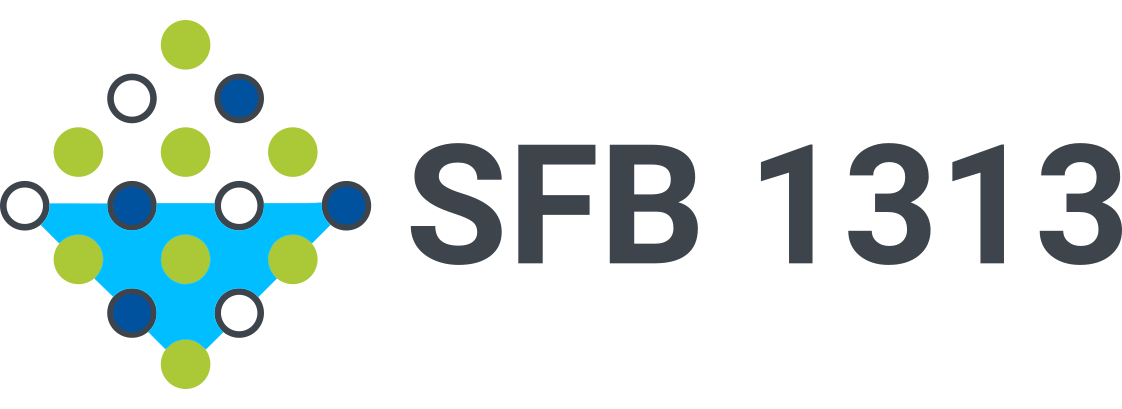
\includegraphics[height=1cm, keepaspectratio]{logosfb.png}\hspace{1cm}%
%	 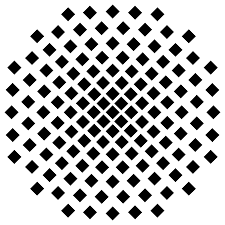
\includegraphics[height=1cm, keepaspectratio]{logostutt.png}}
\date{16th April 2019}
%%%%%%%%%%%%%%%%%%%%%%%%%%%%%%%%%%%%%%%%%%%%%%%%%%%%%%%%%%%%%%%%%%%%%%%%%%%%
\begin{document}
\begin{frame}
	\vspace{0.3cm}
	\centering
	
\includegraphics[height=0.9cm, 
	keepaspectratio]{logopoliblu.png}\hspace{0.5cm}%
	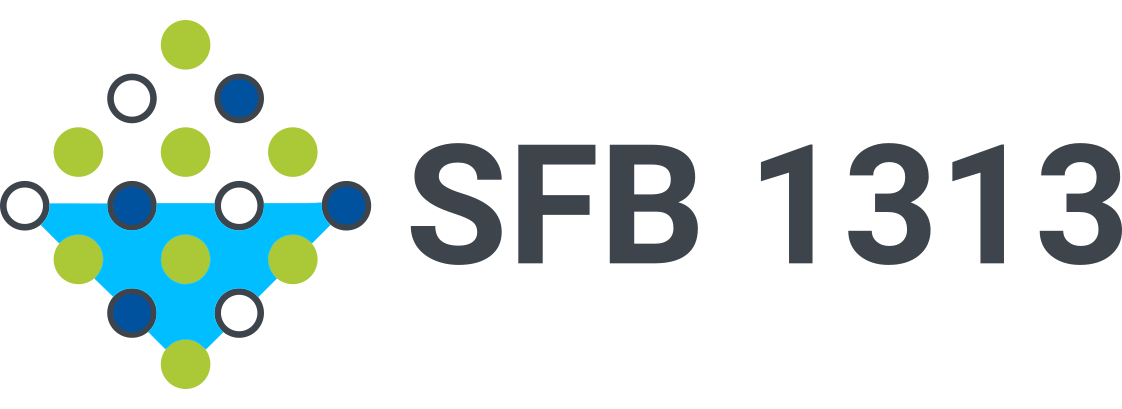
\includegraphics[height=0.9cm, keepaspectratio]{logosfb.png}\hspace{0.5cm}%
	
\includegraphics[height=0.9cm, keepaspectratio]{logostuttnome.png}
	\vspace{0.3cm}
	\setlength\tabcolsep{3pt} % default value: 6pt
	\maketitle
	\setlength\tabcolsep{6pt} % default value: 6pt
\end{frame}
%%%%%%%%%%%%%%%%%%%%%%%%%%%%%%%%%%%%%%%%%%%%%%%%%%%%%%%%%%%%%%%%%%%%%%%%%%%%
\begin{frame}{Introduction}
Coupled \textbf{free-flow} and \textbf{porous-medium flow} systems involve 
complex phenomena acting at different scales:
%\begin{itemize}
%	\item involve complex phenomena acting at different scales
%	\item are important in many applications: soil salinization, PEM fuel cells, ecc.
%\end{itemize}
%	\begin{itemize}
%		\item Coupled free-flow and porous-medium flow systems are common in 
%		many applications: PEM fuel cells, industrial drying processes, soil 
%		evaporation, \dots
%	\end{itemize}
\begin{figure}
	\centering
	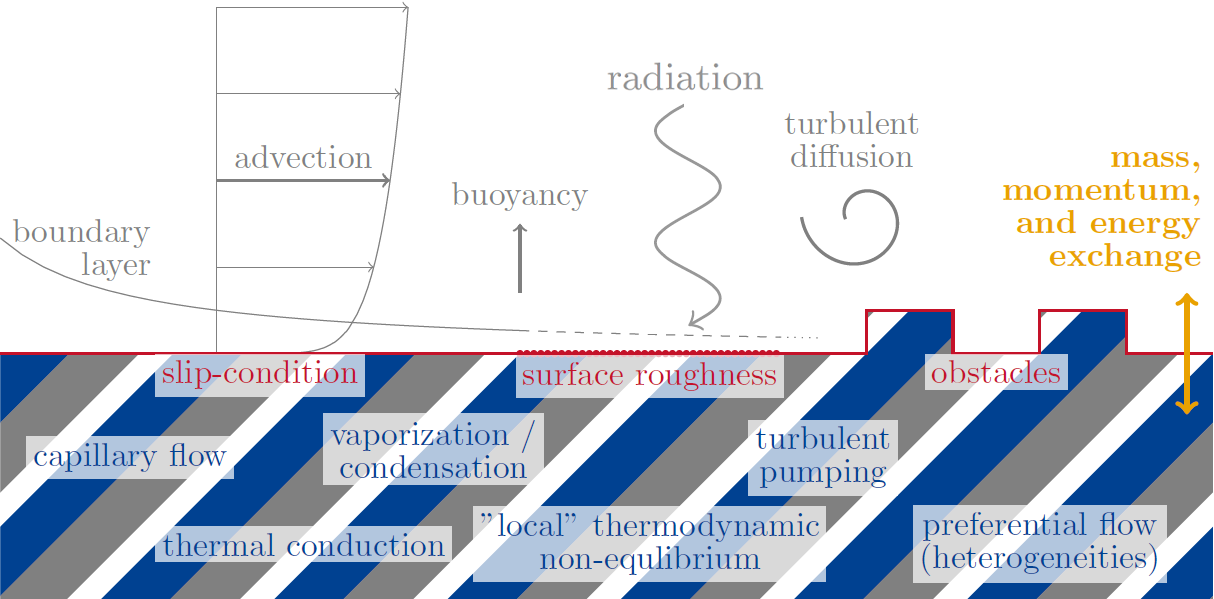
\includegraphics[width=0.8\textwidth]{intropicture2.png}
	\caption{\color{gray}T. Fetzer. Coupled Free and Porous-Medium Flow 
	Processes Affected by Turbulence and Roughness.}
\end{figure}
Applications: soil salinization, PEM fuel cells, drying processes, etc.
\end{frame}
%%%%%%%%%%%%%%%%%%%%%%%%%%%%%%%%%%%%%%%%%%%%%%%%%%%%%%%%%%%%%%%%%%%%%%%%%%%%
\begin{frame}{Introduction}
Several analysis can be found in literature:
\begin{itemize}
	\item single-domain or two-domain approach.
	\item coupling concepts for different levels of complexity.
	\item monolithic or iterative solution procedures.
	\item turbulence and roughness effects.
\end{itemize}
\pause
\vspace{0.5cm}
Considering a \textbf{single-phase}, \textbf{single-component}, \textbf{isothermal fluid}, the aims of this thesis are:
\begin{itemize}
	\item to implement and test \textbf{TVD methods} for the free-flow model.
	\item to study the effect of \textbf{rough interfaces} between the two subdomains of a coupled model.
\end{itemize}
\end{frame}
%%%%%%%%%%%%%%%%%%%%%%%%%%%%%%%%%%%%%%%%%%%%%%%%%%%%%%%%%%%%%%%%%%%%%%%%%%%%
\begin{frame}{Outline}
	\tableofcontents
\end{frame}
%%%%%%%%%%%%%%%%%%%%%%%%%%%%%%%%%%%%%%%%%%%%%%%%%%%%%%%%%%%%%%%%%%%%%%%%%%%%
\section{Governing equations}
\begin{frame}{Free-flow}
Incompressible RANS equations:
\begin{align*}
\nabla \cdot \bar{\mathbf{v}} = 0&\\
\frac{\partial \bar{\mathbf{v}}}{\partial t} + \nabla 
\cdot (\bar{\mathbf{v}} \bar{\mathbf{v}}^\mathrm{T}) - \nabla \cdot 
((\nu + \nu_t) \nabla \bar{\mathbf{v}}) + \frac{1}{\varrho}\nabla (p + \frac{2}{3}\varrho k) = \mathbf{0}&
\end{align*}
$k\text{-}\omega$ turbulence model $\nu_t = k / \tilde{\omega}$ with limiters:
\begin{align*}
&\frac{\partial k}{\partial t} + \nabla \cdot (k\bar{\mathbf{v}}) - \nabla \cdot
\bigg[\bigg(\nu + \sigma^*\frac{k}{\omega}\bigg) \nabla k\bigg] -P + \beta^* k 
\omega = 0\\
%\end{gather*}
%\begin{multline*}
&\frac{\partial \omega}{\partial t} + \nabla \cdot (\omega \bar{\mathbf{v}}) - 
\nabla \cdot \bigg[ \bigg( \nu + \sigma \frac{k}{\omega} \bigg) \nabla \omega 
\bigg]-\\
&\hspace{2.5cm}- \alpha \frac{\omega}{k} 2 \nu_t \bar{\mathbf{S}} \cdot \bar{\mathbf{S}} 
-\frac{\sigma_d}{\omega} \nabla k \cdot 
\nabla \omega+ \beta \omega^2 = 0
\end{align*}
\end{frame}
%%%%%%%%%%%%%%%%%%%%%%%%%%%%%%%%%%%%%%%%%%%%%%%%%%%%%%%%%%%%%%%%%%%%%%%%%%
\begin{frame}{Porous-medium flow - REV scale approach}
Continuity equation for a single-phase incompressible fluid:
\begin{equation*}
\nabla \cdot \mathbf{v} = 0
\end{equation*}
Momentum equation:
\begin{itemize}
	\item Darcy's law:
\begin{equation*}
	\mathbf{v} = -\frac{1}{\mu}\mathbf{K} \nabla p
\end{equation*}
	\item Forchheimer's law:
	\begin{equation*}
	\mathbf{v} + C_F \sqrt{\mathbf{K}} \frac{\varrho}{\mu} |\mathbf{v}| 
	\mathbf{v} = - \frac{1}{\mu}\mathbf{K} \nabla p
	\end{equation*}
	It models a quadratic drag and it holds at \textbf{higher} 
	$\boldsymbol{Re}$ than the Darcy's law.
\end{itemize}
\end{frame}
%%%%%%%%%%%%%%%%%%%%%%%%%%%%%%%%%%%%%%%%%%%%%%%%%%%%%%%%%%%%%%%%%%%%%%%%%
\begin{frame}{Coupling conditions}
%At the interface we apply:
\begin{itemize}
	\item Continuity of normal velocity:
	\begin{equation*}
	[\mathbf{v} \cdot \mathbf{n}]_\text{ff} = - [\mathbf{v} 
	\cdot \mathbf{n}]_\text{pm}
	\end{equation*}
	\item Continuity of normal stresses:
	\begin{equation*}
	[(\varrho \mathbf{v} \mathbf{v}^\mathrm{T} - (\mu + \mu_t) \nabla 
	\mathbf{v} + p\mathbf{I}) 
	\mathbf{n}]_\text{ff} = 
	- [p\mathbf{n}]_\text{pm}
	\end{equation*}
	\item Beavers-Joseph-Saffman condition for the tangential component of 
	momentum:
	\begin{equation*}
	\bigg[ \bigg( -\frac{\sqrt{\mathrm{K}}}{\alpha_\text{BJ}} (\nabla \mathbf{v}) 
	\mathbf{n} - \mathbf{v} \bigg) \cdot \mathbf{t}_i \bigg]_\text{ff} = 0 
	\quad \forall i \in \{1, \dots, dim - 1\}
	\end{equation*}
\end{itemize}
\end{frame}
%%%%%%%%%%%%%%%%%%%%%%%%%%%%%%%%%%%%%%%%%%%%%%%%%%%%%%%%%%%%%%%%%%%%%%%%%%
\section{Numerical model}
\begin{frame}{Finite volumes discretization}
%	\begin{itemize}
%		\item \textbf{Staggered grid} approach in the free-flow:
%		\begin{columns}%
%		\column{0.5\textwidth}%
%		\begin{figure}
%			\centering
%			\includegraphics[%
%			%trim={2cm 1cm 0cm 0cm}, clip, height=0.65\textheight]%
%%			trim={2cm 5.2cm 0cm 0.8cm}, clip, height=0.4\textheight]%
%			trim={2cm 5.2cm 7cm 0.8cm}, clip, height=0.4\textheight]%
%			{staggered_grid_mia.pdf}
%		\end{figure}
%		\column{0.2\textwidth}%
%		Primary variables: $\mathbf{v}$, $p$, $k$, $\omega$
%		\end{columns}%
%		\item \textbf{Cell-centred} approach in the porous-medium flow:
%		\begin{columns}%
%		\column{0.4\textwidth}%
%		\begin{figure}
%%			\centering
%			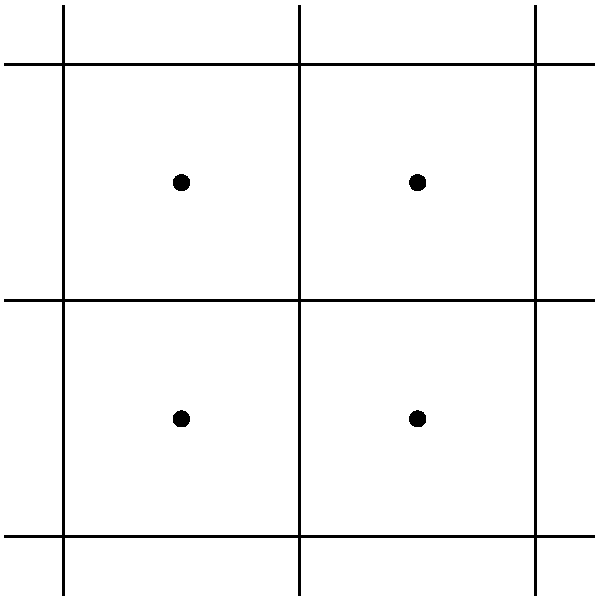
\includegraphics[height=0.3\textheight]{cellcentred.pdf}
%%			\hspace{2cm}
%		\end{figure}
%		\column{0.5\textwidth}%
%		Primary variables: $p$
%		\end{columns}%
%	\end{itemize}
	\begin{itemize}
	\item \textbf{Staggered grid} approach in the free-flow:
	\begin{minipage}{0.5\textwidth}%
		\begin{figure}
			\vspace{0.1cm}
			\centering
			\includegraphics[%
			%trim={2cm 1cm 0cm 0cm}, clip, height=0.65\textheight]%
			%			trim={2cm 5.2cm 0cm 0.8cm}, clip, height=0.4\textheight]%
			trim={2cm 5.2cm 7cm 0.8cm}, clip, height=0.4\textheight]%
			{staggered_grid_mia.pdf}
			\vspace{0.2cm}
		\end{figure}
	\end{minipage}%
	\begin{minipage}{0.5\textwidth}
		\centering
		Scalar primary variables:\\
		$p$, $k$, $\omega$\\
		Vectorial primary variables:\\
		$\mathbf{v}=[u,v]^\mathrm{T}$
	\end{minipage}
	\item \textbf{Cell-centred} approach in the porous-medium flow:
	\begin{minipage}{0.5\textwidth}%
		\begin{figure}
			\vspace{0.1cm}
			%			\centering
			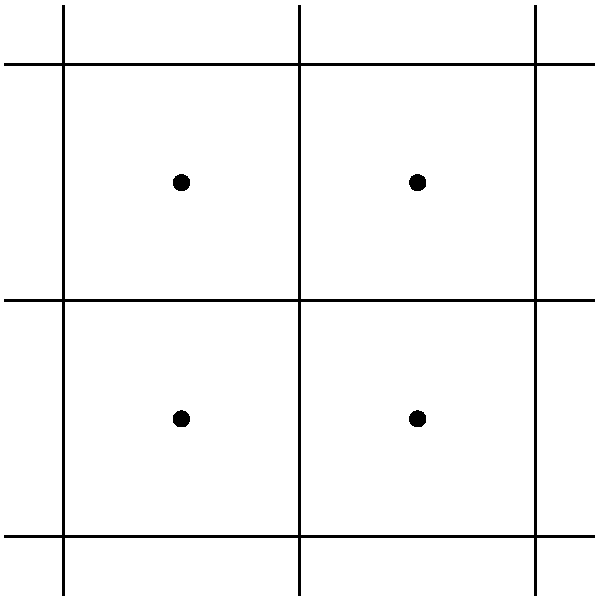
\includegraphics[height=0.3\textheight]{cellcentred.pdf}
			%			\hspace{2cm}
		\end{figure}
	\end{minipage}%
	\begin{minipage}{0.5\textwidth}
		\centering
		Scalar primary variables:\\
		$p$
	\end{minipage}%
\end{itemize}
\end{frame}
%%%%%%%%%%%%%%%%%%%%%%%%%%%%%%%%%%%%%%%%%%%%%%%%%%%%%%%%%%%%%%%%%%%%%%%%%
\begin{frame}{Differencing schemes}
Non-linear convective term of the Navier-Stokes equations:
\begin{equation*}
\int_V \nabla \cdot (\mathbf{v} \mathbf{v}^\mathrm{T}) \; dV = \int_{\partial 
V} 
\overbrace{\mathbf{v}}^{\substack{\text{\makebox[0pt]{transported}} 
		\\ \text{\makebox[0pt]{field}}}} \underbrace{(\mathbf{v} \cdot 
	\mathbf{n})}_{\substack{\text{\makebox[0pt]{transporting}} \\
		\text{\makebox[0pt]{velocity}}}} \; dA
\end{equation*}
Differencing scheme needed to approximate the transported field:
\begin{itemize}
	\item Upwind $\rightarrow$ $1^\text{st}$ order, stable, high numerical dissipation.
	\item LUD, QUICK, etc. $\rightarrow$ $2^\text{nd}$ or $3^\text{rd}$ order, unphysical oscillations.
	\item \textbf{TVD methods $\rightarrow$ 2$^\text{nd}$ order, non-linear, 
	oscillation-free}.\\
	\emph{Flux limiters: Van Leer, Min-Mod, Van Alabada, etc.}
\end{itemize}
\end{frame}
%%%%%%%%%%%%%%%%%%%%%%
%\begin{frame}{TVD methods}
%	immagine, formula
%\end{frame}
%%%%%%%%%%%%%%%%%%%%%%%%%%%%%%%%%%%%%%%%%%%%%%%%%%%%%%%%%%%%%%%%%%%%%
\begin{frame}{Resulting equations}
\begin{itemize}
\item After having performed the spatial discretization, we obtain a system of 
ODEs, which is solved using \textbf{implicit unconditionally stable} methods 
(BDF2 or Backward Euler).
\vspace{0.5cm}

\item The resulting non-linear algebraic system is solved 
\textbf{monolithically}, 
employing the \textbf{Newton's method}. The entries of the Jacobian matrix are 
computed numerically using finite differences.
\vspace{0.5cm}

\item Eventually, the linear system is solved directly using the library 
UMFPACK.
\end{itemize}
\end{frame}
%%%%%%%%%%%%%%%%%%%%%%%%%%%%%%%%%%%%%%%%%%%%%%%%%%%%%%%%%%%%%%%%%%%%%%%%
\section{Numerical results}
\begin{frame}{Free-flow validation tests}
\begin{itemize}
	\item Convergence tests refining the grid, using Navier-Stokes problems 
	with analytical solution.
	\vspace{-0.3cm}
	\begin{table}\scriptsize
		\[
		\begin{array}{c|ccc}
		\toprule
		& \text{Upwind} & \text{Min-Mod} & \text{Van Leer} \\ 
		\midrule
		p & 1.148 & 1.659 & 1.058\\
		u & 1.071 & 1.441 & 1.437\\
		v & 1.068 & 1.533 & 1.560\\
		\bottomrule
		\end{array}
		\]
%		\caption{\tiny Convergence orders with $Re = 1000$}
	\end{table}
	\item Backward facing step test: comparison with the NASA CFL3D code, at 
	$Re_H=36000$.
	\begin{figure}
		\centering
		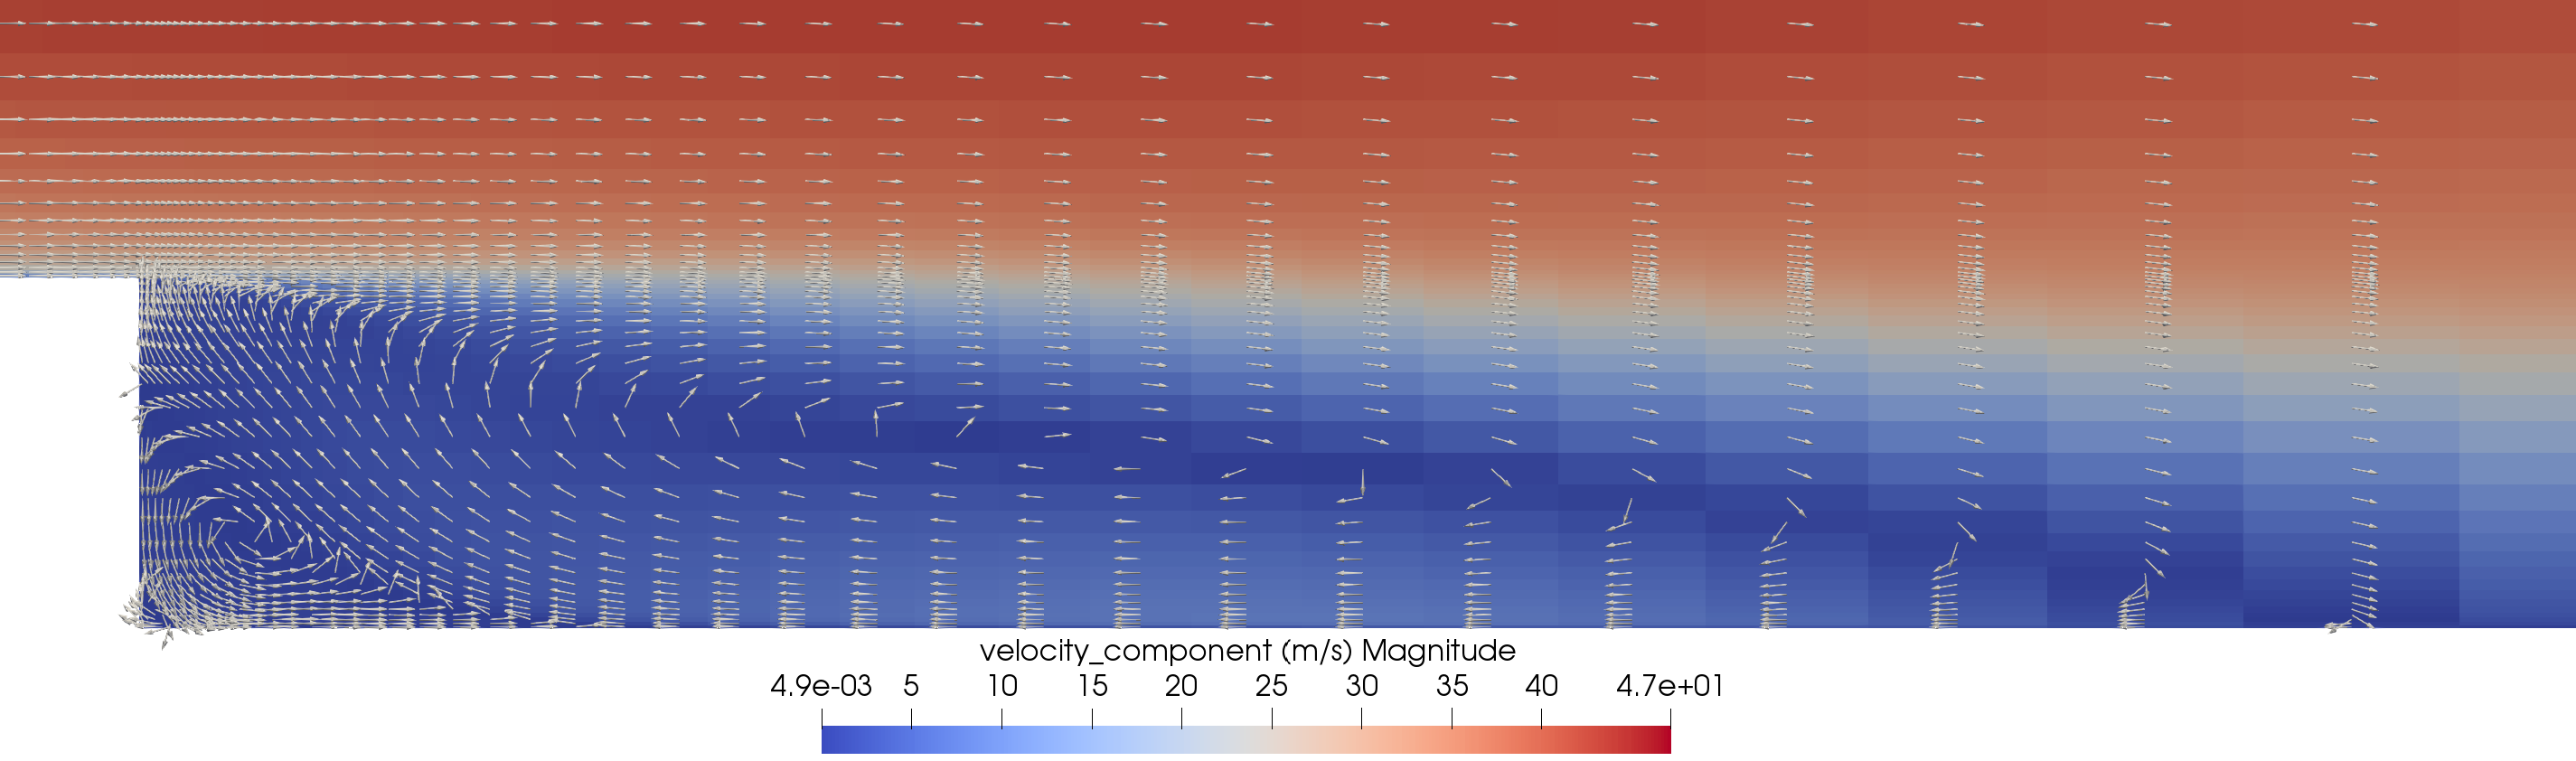
\includegraphics[width=0.9\textwidth]{bfs_glimphs.png}
	\end{figure}
\end{itemize}
\end{frame}
%%%%%%%%%%%%%%%%%
%\begin{frame}{Spatial convergence - steady SinCos problem}
%\vspace{-0.8cm}
%\begin{figure}
%	\centering
%	\subfloat[\tiny Figure: Upwind, 
%	
%$Re=1000$]{\hspace{-0.5cm}% This file was created by matlab2tikz.
%
\definecolor{mycolor1}{rgb}{0.00000,0.44700,0.74100}%
\definecolor{mycolor2}{rgb}{0.85000,0.32500,0.09800}%
\definecolor{mycolor3}{rgb}{0.92900,0.69400,0.12500}%
%
\begin{tikzpicture}

\begin{axis}[%
width=0.951\figwidth,
height=0.75\figwidth,
at={(0\figwidth,0\figwidth)},
scale only axis,
xmode=log,
xmin=4,
xmax=100,
xminorticks=true,
ymode=log,
ymin=0.00266295649,
ymax=0.1,
yminorticks=true,
ylabel style={font=\color{white!15!black}\scriptsize},
ylabel={$L^2$-error},
axis background/.style={fill=white},
legend style={at={(0.03,0.03)}, anchor=south west, legend cell align=left, 
align=left, font=\scriptsize}
]
\addplot [color=mycolor1, mark=x, mark options={solid, mycolor1}]
  table[row sep=crcr]{%
4	0.0596083589\\
8	0.0364982308\\
16	0.0196434526\\
32	0.00962257784\\
64	0.00434161729\\
};
\addlegendentry{$p$}

\addplot [color=mycolor2, mark=x, mark options={solid, mycolor2}]
  table[row sep=crcr]{%
4	0.0339372138\\
8	0.0206751686\\
16	0.011131246\\
32	0.00559430586\\
64	0.00266295649\\
};
\addlegendentry{$u$}

\addplot [color=mycolor3, mark=x, mark options={solid, mycolor3}]
  table[row sep=crcr]{%
4	0.0347600515\\
8	0.0213374017\\
16	0.0114856296\\
32	0.00577467407\\
64	0.00275450966\\
};
\addlegendentry{$v$}

\addplot [color=white!70!black, forget plot]
  table[row sep=crcr]{%
4	0.06657391225\\
100	0.00266295649\\
};
\addplot [color=white!70!black, forget plot]
  table[row sep=crcr]
%	\subfloat[\tiny Figure: Min-Mod, 
%	$Re=1000$]{% This file was created by matlab2tikz.
%
\definecolor{mycolor1}{rgb}{0.00000,0.44700,0.74100}%
\definecolor{mycolor2}{rgb}{0.85000,0.32500,0.09800}%
\definecolor{mycolor3}{rgb}{0.92900,0.69400,0.12500}%
%
\begin{tikzpicture}

\begin{axis}[%
width=0.951\figwidth,
height=0.75\figwidth,
at={(0\figwidth,0\figwidth)},
scale only axis,
xmode=log,
xmin=4,
xmax=100,
xminorticks=true,
ymode=log,
ymin=0.0001,
ymax=0.0206930353,
yminorticks=true,
ylabel style={font=\color{white!15!black}\scriptsize},
ylabel={$L^2$-error},
axis background/.style={fill=white},
legend style={at={(0.03,0.03)}, anchor=south west, legend cell align=left, 
align=left, font=\scriptsize}
]
\addplot [color=mycolor1, mark=x, mark options={solid, mycolor1}]
  table[row sep=crcr]{%
4	0.0206930353\\
8	0.0102262223\\
16	0.00364544433\\
32	0.000812298263\\
64	0.000257143964\\
};
\addlegendentry{$p$}

\addplot [color=mycolor2, mark=x, mark options={solid, mycolor2}]
  table[row sep=crcr]{%
4	0.0130268788\\
8	0.00605072242\\
16	0.00243635311\\
32	0.000918041806\\
64	0.000338134479\\
};
\addlegendentry{$u$}

\addplot [color=mycolor3, mark=x, mark options={solid, mycolor3}]
  table[row sep=crcr]{%
4	0.0129926934\\
8	0.00750558766\\
16	0.0037160882\\
32	0.00148526754\\
64	0.000512917943\\
};
\addlegendentry{$v$}

\addplot [color=white!70!black, forget plot]
  table[row sep=crcr]{%
4	0.0025\\
100	0.0001\\
};
\addplot [color=white!70!black, forget plot]
  table[row sep=crcr]
%\end{figure}
%\vspace{-0.3cm}
%\begin{table}\footnotesize
%	\[
%	\begin{array}{c|ccc}
%	\toprule
%	& \text{Upwind} & \text{Min-Mod} & \text{Van Leer} \\ 
%	\midrule
%	p & 1.148 & 1.659 & 1.058\\
%	u & 1.071 & 1.441 & 1.437\\
%	v & 1.068 & 1.533 & 1.560\\
%	\bottomrule
%	\end{array}
%	\]
%	\caption{\tiny Convergence orders with $Re = 1000$}
%\end{table}
%\end{frame}
%%%%%%%%%%%%%%%%%%%%%%%%%%%%%%%%%%%%%%%%%%%%%%%%%%%%%%%%%%%%%%%%%%%%%%%%%%%%
%\begin{frame}{Backward facing step}
%\begin{figure}
%	\centering
%	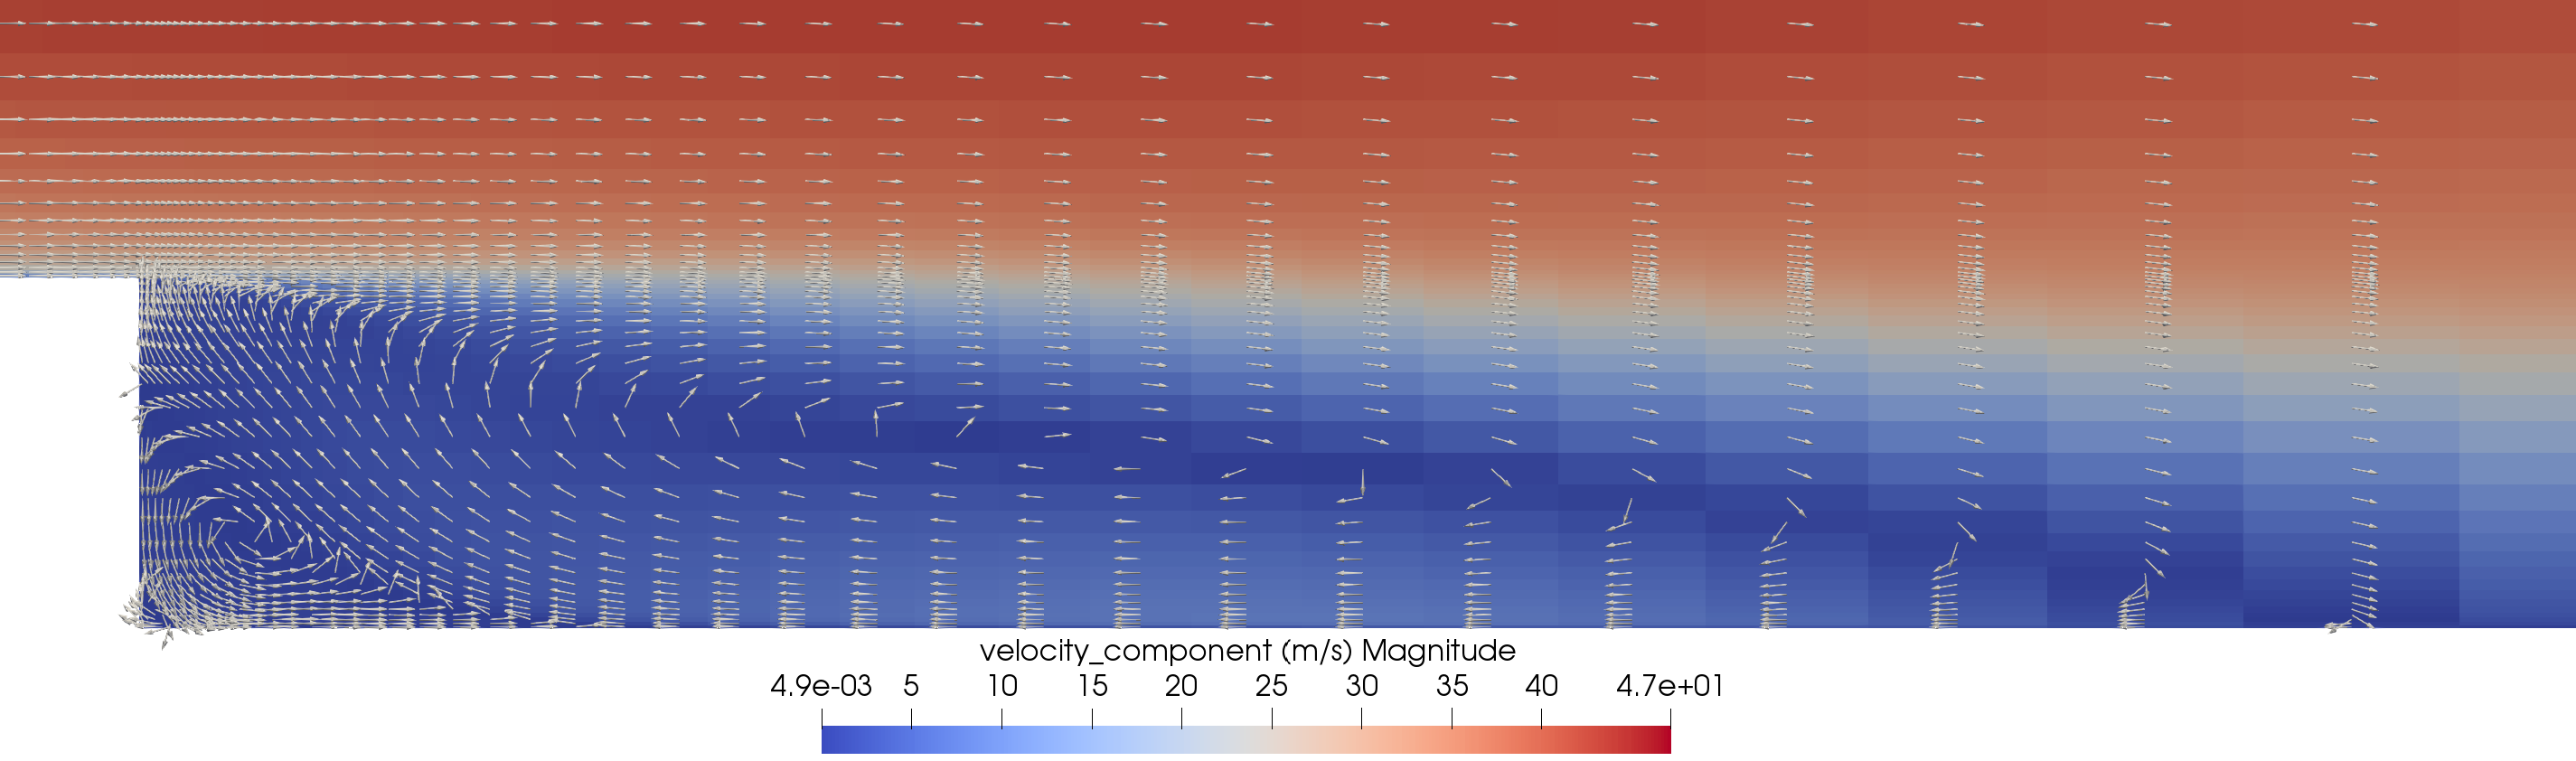
\includegraphics[width=\textwidth]{bfs_glimphs.png}
%\end{figure}
%\vspace{0.5cm}
%\begin{itemize}
%	\item $Re_H = 36000$, based on the step height $H$.
%	\item Results comparison with the NASA CFL3D code, from 
%	{\small \url{https://turbmodels.larc.nasa.gov/backstep_val.html}}.
%\end{itemize}
%
%\end{frame}
%%%%%%%%%%%%%%%%%%%%%%%%%%%%%%%%%%%%%%%%%%%%%%%%%%%%%%%%%%%%%%%%%%%%%%%%%%%%
%\begin{frame}{Backward facing step - friction coefficient}
%\begin{figure}
%	\centering
%	% This file was created by matlab2tikz.
%
\definecolor{mycolor4}{rgb}{0.00000,0.44700,0.74100}%
\definecolor{mycolor3}{rgb}{0.85000,0.32500,0.09800}%
\definecolor{mycolor2}{rgb}{0.92900,0.69400,0.12500}%
\definecolor{mycolor1}{rgb}{0.49400,0.18400,0.55600}%
%
\begin{tikzpicture}

\begin{axis}[%
width=0.951\bfswidth,
height=0.75\bfsheight,
at={(0\bfswidth,0\bfsheight)},
scale only axis,
xmin=0,
xmax=30,
xlabel style={font=\color{white!15!black}},
xlabel={$x/H$},
ymin=-0.0015,
ymax=0.003,
ylabel style={font=\color{white!15!black}, rotate=-90},
ylabel={$C_f$},
axis background/.style={fill=white},
legend style={at={(0.97,0.03)}, anchor=south east, legend cell align=left, align=left, draw=white!15!black, font=\scriptsize}
]
\addplot [color=mycolor1]
  table[row sep=crcr]{%
-126.659821	0\\
-123.869415	0\\
-121.536697	0\\
-119.584694	0\\
-117.948982	0\\
-116.575592	0\\
-115.419197	0\\
-114.441628	0\\
-113.610641	0\\
-112.898804	0\\
-112.282623	0\\
-111.741768	0\\
-111.258392	0\\
-110.816551	0\\
-110.401649	0\\
-110	0.00812491402\\
-109.598709	0.0107412264\\
-109.192223	0.00526966201\\
-108.78054	0.00532762799\\
-108.363647	0.00526078884\\
-107.941513	0.00510590943\\
-107.514137	0.00494101224\\
-107.081512	0.00479498133\\
-106.643623	0.00467133615\\
-106.20047	0.00456604315\\
-105.752045	0.00447485177\\
-105.298347	0.00439458713\\
-104.839378	0.00432301546\\
-104.375137	0.00425852556\\
-103.90564	0.00419991836\\
-103.430878	0.00414627325\\
-102.950867	0.00409686565\\
-102.465614	0.00405111257\\
-101.975151	0.00400854275\\
-101.479469	0.00396876922\\
-100.978607	0.00393147068\\
-100.47258	0.00389637472\\
-99.9614029	0.00386324921\\
-99.4451218	0.00383189856\\
-98.9237442	0.00380215677\\
-98.3973236	0.00377388159\\
-97.8658752	0.0037469489\\
-97.3294449	0.00372125208\\
-96.7880783	0.00369669567\\
-96.2418137	0.00367319607\\
-95.6906891	0.00365067925\\
-95.1347656	0.00362907816\\
-94.5740891	0.00360833248\\
-94.0087128	0.00358838751\\
-93.4386978	0.00356919412\\
-92.8640976	0.00355070736\\
-92.2849731	0.00353288511\\
-91.7014008	0.00351568731\\
-91.1134415	0.00349907787\\
-90.5211716	0.00348302512\\
-89.9246597	0.00346749928\\
-89.3239822	0.00345247402\\
-88.719223	0.0034379235\\
-88.110466	0.00342382537\\
-87.4977875	0.00341015938\\
-86.881279	0.00339690736\\
-86.2610397	0.00338405324\\
-85.637146	0.00337158027\\
-85.0097122	0.00335947261\\
-84.3788223	0.00334771629\\
-83.7445831	0.00333629688\\
-83.1070938	0.00332519948\\
-82.4664688	0.00331441243\\
-81.8228073	0.00330392155\\
-81.1762238	0.00329371286\\
-80.526825	0.00328377704\\
-79.8747253	0.00327410363\\
-79.2200546	0.00326468237\\
-78.5629196	0.00325550698\\
-77.9034424	0.00324657047\\
-77.241745	0.003237864\\
-76.5779495	0.00322938082\\
-75.9121857	0.0032211158\\
-75.2445755	0.00321306172\\
-74.5752563	0.00320521113\\
-73.9043503	0.00319755822\\
-73.2319946	0.00319009693\\
-72.5583191	0.00318281981\\
-71.8834457	0.00317571987\\
-71.2075272	0.00316879246\\
-70.5306931	0.00316203269\\
-69.8530731	0.00315543427\\
-69.1748047	0.00314899208\\
-68.4960327	0.00314270402\\
-67.8168869	0.00313656661\\
-67.1375122	0.00313057564\\
-66.4580383	0.0031247267\\
-65.7786026	0.00311901676\\
-65.0993576	0.00311344303\\
-64.4204254	0.00310800201\\
-63.741951	0.00310268928\\
-63.0640717	0.00309750182\\
-62.3869247	0.00309243705\\
-61.71064	0.0030874915\\
-61.0353584	0.00308266166\\
-60.3612175	0.00307794265\\
-59.688343	0.0030733312\\
-59.0168724	0.00306882523\\
-58.3469391	0.00306442217\\
-57.678669	0.00306011969\\
-57.0121956	0.00305591547\\
-56.3476448	0.00305180787\\
-55.6851387	0.00304779573\\
-55.0248108	0.00304387836\\
-54.3667717	0.00304005388\\
-53.7111549	0.00303631951\\
-53.0580711	0.00303267338\\
-52.4076424	0.00302911317\\
-51.7599831	0.00302563724\\
-51.1152	0.0030222442\\
-50.4734154	0.00301893149\\
-49.8347282	0.00301569654\\
-49.1992493	0.00301253749\\
-48.5670853	0.00300945179\\
-47.9383316	0.00300643826\\
-47.3130913	0.00300349738\\
-46.6914597	0.00300062844\\
-46.0735283	0.00299783028\\
-45.4593964	0.00299510267\\
-44.849144	0.00299244514\\
-44.2428665	0.00298985722\\
-43.6406364	0.002987338\\
-43.0425415	0.00298488676\\
-42.448658	0.00298250164\\
-41.8590622	0.00298017892\\
-41.2738228	0.0029779172\\
-40.6930161	0.00297571463\\
-40.1166992	0.00297357049\\
-39.5449448	0.00297148456\\
-38.9778061	0.00296945591\\
-38.4153481	0.00296748523\\
-37.8576202	0.00296557252\\
-37.3046799	0.00296371733\\
-36.7565765	0.00296191871\\
-36.2133522	0.00296017667\\
-35.6750526	0.00295849098\\
-35.1417198	0.0029568607\\
-34.6133919	0.0029552842\\
-34.090107	0.00295375939\\
-33.5718956	0.00295228465\\
-33.0587883	0.00295085786\\
-32.5508118	0.00294947741\\
-32.0479965	0.00294814096\\
-31.5503578	0.00294684642\\
-31.0579185	0.00294559239\\
-30.5706959	0.00294437679\\
-30.088707	0.00294319773\\
-29.6119614	0.0029420529\\
-29.1404705	0.00294093997\\
-28.674242	0.00293985684\\
-28.2132816	0.00293880119\\
-27.7575932	0.00293777138\\
-27.3071766	0.00293676602\\
-26.8620319	0.0029357837\\
-26.4221554	0.00293482305\\
-25.9875412	0.00293388264\\
-25.5581837	0.0029329625\\
-25.1340733	0.00293206167\\
-24.7151985	0.00293117925\\
-24.3015461	0.00293031475\\
-23.8931046	0.00292946748\\
-23.4898529	0.0029286372\\
-23.0917759	0.00292782346\\
-22.6988544	0.00292702671\\
-22.3110657	0.00292624743\\
-21.9283867	0.00292548537\\
-21.5507946	0.00292474148\\
-21.1782646	0.00292401621\\
-20.8107681	0.0029233091\\
-20.4482784	0.00292261993\\
-20.090765	0.00292194868\\
-19.7381973	0.00292129512\\
-19.390543	0.00292065926\\
-19.0477715	0.00292004109\\
-18.7098465	0.00291944086\\
-18.3767338	0.00291885855\\
-18.0483971	0.00291829486\\
-17.724802	0.00291774957\\
-17.4059086	0.00291722314\\
-17.0916805	0.00291671581\\
-16.7820759	0.00291622779\\
-16.4770565	0.00291575934\\
-16.1765823	0.00291531067\\
-15.8806124	0.00291488227\\
-15.5891027	0.00291447458\\
-15.3020134	0.00291408808\\
-15.0193014	0.00291372347\\
-14.7409229	0.00291338144\\
-14.4668341	0.00291306223\\
-14.196991	0.0029127663\\
-13.9313507	0.00291249412\\
-13.6698666	0.00291224592\\
-13.4124956	0.00291202264\\
-13.1591911	0.0029118245\\
-12.9099083	0.00291165197\\
-12.6646013	0.00291150599\\
-12.4232244	0.00291138724\\
-12.1857328	0.00291129644\\
-11.9520798	0.00291123404\\
-11.7222185	0.00291120075\\
-11.4961042	0.00291119749\\
-11.2736912	0.00291122473\\
-11.0549326	0.00291128294\\
-10.8397818	0.00291137281\\
-10.6281948	0.00291149481\\
-10.4201241	0.00291165011\\
-10.2155237	0.00291183894\\
-10.0143499	0.00291206199\\
-9.81655598	0.00291231996\\
-9.62209702	0.00291261333\\
-9.43092823	0.00291294302\\
-9.24300289	0.00291330973\\
-9.05827904	0.00291371392\\
-8.87670994	0.00291415653\\
-8.69825268	0.00291463826\\
-8.52286243	0.0029151598\\
-8.35049629	0.00291572185\\
-8.18111134	0.00291632535\\
-8.01466274	0.00291697076\\
-7.85110855	0.00291765877\\
-7.6904068	0.00291839032\\
-7.53251457	0.00291916542\\
-7.37739086	0.00291998521\\
-7.22499323	0.00292085018\\
-7.07528162	0.00292176055\\
-6.92821455	0.00292271702\\
-6.78375196	0.00292372005\\
-6.64185381	0.00292477012\\
-6.50248051	0.00292586791\\
-6.36559296	0.00292701321\\
-6.23115158	0.00292820693\\
-6.09911919	0.00292944931\\
-5.96945667	0.00293074059\\
-5.84212732	0.00293208123\\
-5.71709299	0.00293347123\\
-5.59431791	0.00293491129\\
-5.4737649	0.00293640164\\
-5.35539818	0.00293794251\\
-5.23918247	0.00293953391\\
-5.12508249	0.0029411763\\
-5.01306343	0.00294286991\\
-4.90309095	0.00294461497\\
-4.79513168	0.00294641219\\
-4.68915176	0.00294826343\\
-4.58511829	0.00295017194\\
-4.48299885	0.00295213982\\
-4.382761	0.002954175\\
-4.28437376	0.00295626209\\
-4.1878047	0.00295845093\\
-4.09302378	0.00296068029\\
-3.9079206	0.00296474434\\
-3.8178525	0.00296697603\\
-3.72974896	0.0029693353\\
-3.64356518	0.00297174184\\
-3.55925632	0.00297418959\\
-3.47677946	0.00297667691\\
-3.3960917	0.0029792022\\
-3.31715178	0.00298176566\\
-3.23991895	0.00298436778\\
-3.16435361	0.00298700784\\
-3.09041691	0.00298968609\\
-3.01807046	0.0029924023\\
-2.94727731	0.00299515552\\
-2.87800097	0.00299794599\\
-2.8102057	0.00300077302\\
-2.74385667	0.00300363614\\
-2.67891979	0.00300653558\\
-2.61536169	0.00300947018\\
-2.55314946	0.0030124404\\
-2.4922514	0.00301544531\\
-2.43263578	0.00301848515\\
-2.37427211	0.00302155921\\
-2.31713033	0.00302466773\\
-2.26118088	0.00302781072\\
-2.20639539	0.00303098792\\
-2.15274525	0.00303419912\\
-2.10020328	0.00303744478\\
-2.04874182	0.00304072467\\
-1.99833488	0.00304403901\\
-1.94895637	0.00304738805\\
-1.90058088	0.00305077201\\
-1.85318351	0.00305419113\\
-1.80673993	0.0030576461\\
-1.76122606	0.00306113739\\
-1.71661866	0.00306466524\\
-1.67289472	0.00306823081\\
-1.6300317	0.00307183457\\
-1.58800757	0.00307547743\\
-1.54680061	0.00307916035\\
-1.50638986	0.00308288448\\
-1.4667542	0.00308665098\\
-1.42787349	0.00309046102\\
-1.38972759	0.00309431623\\
-1.35229695	0.00309821824\\
-1.31556225	0.00310216891\\
-1.27950454	0.00310616987\\
-1.24410546	0.00311022368\\
-1.20934653	0.00311433244\\
-1.17521	0.00311849872\\
-1.14167821	0.00312272529\\
-1.10873413	0.00312701496\\
-1.07636058	0.00313137146\\
-1.044541	0.00313579803\\
-1.01325893	0.00314029888\\
-0.982498348	0.0031448782\\
-0.952243388	0.00314954109\\
-0.922478497	0.00315429224\\
-0.893188357	0.00315913791\\
-0.864357948	0.00316408416\\
-0.835972309	0.00316913798\\
-0.808016896	0.00317430706\\
-0.780477345	0.00317959976\\
-0.753339469	0.00318502542\\
-0.726589322	0.00319059473\\
-0.700213075	0.0031963191\\
-0.674197137	0.00320221158\\
-0.648528218	0.00320828636\\
-0.623193085	0.00321456022\\
-0.598178685	0.0032210513\\
-0.573472083	0.00322778057\\
-0.549060643	0.00323477224\\
-0.524931729	0.00324205426\\
-0.501073003	0.00324965874\\
-0.477472156	0.00325762248\\
-0.45411703	0.00326598808\\
-0.430995613	0.00327480235\\
-0.408095986	0.00328411651\\
-0.385406405	0.0032939876\\
-0.362915158	0.0033044836\\
-0.340610713	0.00331569812\\
-0.318481535	0.0033277825\\
-0.296516269	0.00334099052\\
-0.274703592	0.00335572776\\
-0.253032297	0.00337256398\\
-0.231491223	0.00339211733\\
-0.210069284	0.00341471471\\
-0.188755453	0.00343966973\\
-0.167538762	0.00346435932\\
-0.146408305	0.0034830512\\
-0.125353187	0.00348763168\\
-0.104362577	0.00346867344\\
-0.0834256858	0.00342689571\\
-0.0625317246	0.00336531037\\
-0.0416699462	0.00340168481\\
-0.0208296124	0.00578542007\\
0.020833334	-4.52145832e-06\\
0.0416666679	-3.42311e-06\\
0.0625	-2.00077451e-07\\
0.0833333358	3.064677e-06\\
0.104166664	6.23515825e-06\\
0.125	9.51022503e-06\\
0.145833328	1.28798602e-05\\
0.166666672	1.63185905e-05\\
0.1875	1.97527006e-05\\
0.208333328	2.31022077e-05\\
0.229166672	2.62824415e-05\\
0.25	2.92147524e-05\\
0.270833343	3.183015e-05\\
0.291666657	3.40725564e-05\\
0.3125	3.59014593e-05\\
0.333333343	3.72919931e-05\\
0.354166657	3.82353537e-05\\
0.375	3.87377113e-05\\
0.395833343	3.88185836e-05\\
0.416666657	3.85091626e-05\\
0.4375	3.78495461e-05\\
0.458333343	3.68872243e-05\\
0.479166657	3.56738892e-05\\
0.5	3.42642124e-05\\
0.520833313	3.27134367e-05\\
0.541666687	3.10765463e-05\\
0.5625	2.93949488e-05\\
0.583333313	2.7688493e-05\\
0.604166687	2.59886419e-05\\
0.625	2.43557133e-05\\
0.645833313	2.28589433e-05\\
0.666666687	2.15681812e-05\\
0.6875	2.05509914e-05\\
0.708333313	1.98652106e-05\\
0.729166687	1.95579523e-05\\
0.75	1.96612782e-05\\
0.770833313	2.01880248e-05\\
0.791666687	2.11330134e-05\\
0.8125	2.24741361e-05\\
0.833333313	2.41739781e-05\\
0.854166687	2.61832392e-05\\
0.875	2.84460075e-05\\
0.895833313	3.09032985e-05\\
0.916666687	3.34949291e-05\\
0.9375	3.61627681e-05\\
0.958333313	3.88550434e-05\\
0.979166687	4.15276518e-05\\
1	4.41418997e-05\\
1.02083337	4.66661986e-05\\
1.04166663	4.90807761e-05\\
1.0625	5.13741543e-05\\
1.08333337	5.35380932e-05\\
1.10416663	5.55709266e-05\\
1.125	5.74828264e-05\\
1.14583337	5.92902179e-05\\
1.16666663	6.09998388e-05\\
1.1875	6.26017063e-05\\
1.20833337	6.4070824e-05\\
1.22916663	6.53640236e-05\\
1.25	6.64146573e-05\\
1.27083337	6.71293965e-05\\
1.29166663	6.7386005e-05\\
1.3125	6.70321242e-05\\
1.33333337	6.58876452e-05\\
1.35416663	6.37520934e-05\\
1.375	6.04171473e-05\\
1.39583337	5.56824234e-05\\
1.41666663	4.9373255e-05\\
1.4375	4.13576272e-05\\
1.45833337	3.15600082e-05\\
1.47916663	1.99701608e-05\\
1.5	6.6458897e-06\\
1.52083337	-8.28979046e-06\\
1.54166663	-2.46563213e-05\\
1.5625	-4.22275407e-05\\
1.58333337	-6.07469265e-05\\
1.60416663	-7.99442714e-05\\
1.625	-9.95522205e-05\\
1.64583337	-0.000119321041\\
1.66666663	-0.000139030541\\
1.6875	-0.000158498267\\
1.70833337	-0.000177583803\\
1.72916663	-0.000196188877\\
1.75	-0.000214254105\\
1.77083337	-0.000231753453\\
1.79166663	-0.000248687546\\
1.8125	-0.000265076727\\
1.83333337	-0.000280954264\\
1.85416663	-0.000296360726\\
1.875	-0.000311339449\\
1.89583337	-0.000325933564\\
1.91666663	-0.000340183906\\
1.9375	-0.000354128017\\
1.95833337	-0.000367799483\\
1.97916663	-0.000381228165\\
2	-0.000394440343\\
2.02083325	-0.000407459156\\
2.04166675	-0.000420304859\\
2.0625	-0.000432995177\\
2.08333325	-0.000445545651\\
2.10416675	-0.000457969873\\
2.125	-0.000470279716\\
2.14583325	-0.000482485397\\
2.16666675	-0.000494595675\\
2.1875	-0.00050661806\\
2.20833325	-0.000518559013\\
2.22916675	-0.000530423771\\
2.25	-0.000542216934\\
2.27083325	-0.000553941994\\
2.29166675	-0.000565602095\\
2.3125	-0.000577199622\\
2.33333325	-0.000588736671\\
2.35416675	-0.00060021464\\
2.375	-0.000611634809\\
2.39583325	-0.000622998108\\
2.41666675	-0.000634305296\\
2.4375	-0.000645556778\\
2.45833325	-0.000656752964\\
2.47916675	-0.00066789391\\
2.5	-0.000678979675\\
2.52083325	-0.000690010027\\
2.54166675	-0.000700984732\\
2.5625	-0.000711903209\\
2.58333325	-0.000722764933\\
2.60416675	-0.000733568973\\
2.625	-0.00074431434\\
2.64583325	-0.00075499987\\
2.66666675	-0.000765624165\\
2.6875	-0.000776185654\\
2.70833325	-0.000786682649\\
2.72916675	-0.000797113054\\
2.75	-0.000807474891\\
2.77083325	-0.000817765831\\
2.79166675	-0.000827983546\\
2.8125	-0.000838125416\\
2.83333325	-0.000848188938\\
2.85416675	-0.000858171319\\
2.875	-0.000868069939\\
2.89583325	-0.000877882005\\
2.91666675	-0.00088760478\\
2.9375	-0.000897235645\\
2.95833325	-0.000906771864\\
2.97916675	-0.000916210993\\
3	-0.000925550528\\
3.02083325	-0.000934788026\\
3.04166675	-0.000943921274\\
3.0625	-0.000952948001\\
3.08333325	-0.000961866172\\
3.10416675	-0.000970673631\\
3.125	-0.000979368459\\
3.14583325	-0.000987948733\\
3.16666675	-0.000996412593\\
3.1875	-0.00100475841\\
3.20833325	-0.0010129842\\
3.22916675	-0.00102108845\\
3.25	-0.0010290693\\
3.27083325	-0.00103692524\\
3.29166675	-0.00104465452\\
3.3125	-0.00105225539\\
3.33333325	-0.00105972611\\
3.35416675	-0.00106706505\\
3.375	-0.00107427035\\
3.39583325	-0.00108134025\\
3.41666675	-0.00108827266\\
3.4375	-0.00109506585\\
3.45833325	-0.00110171793\\
3.47916675	-0.00110822672\\
3.5	-0.00111459021\\
3.52083325	-0.00112080644\\
3.54166675	-0.00112687331\\
3.5625	-0.00113278872\\
3.58333325	-0.00113855058\\
3.60416675	-0.00114415679\\
3.625	-0.00114960549\\
3.64583325	-0.00115489447\\
3.66666675	-0.00116002187\\
3.6875	-0.0011649857\\
3.70833325	-0.00116978423\\
3.72916675	-0.00117441558\\
3.75	-0.00117887824\\
3.77083325	-0.00118317036\\
3.79166675	-0.00118729053\\
3.8125	-0.00119123724\\
3.83333325	-0.00119500922\\
3.85416675	-0.00119860494\\
3.875	-0.00120202336\\
3.89583325	-0.00120526319\\
3.91666675	-0.00120832329\\
3.9375	-0.0012112027\\
3.95833325	-0.0012139004\\
3.97916675	-0.0012164152\\
4	-0.0012187463\\
4.02083349	-0.00122089253\\
4.04166651	-0.0012228532\\
4.0625	-0.00122462725\\
4.08333349	-0.00122621353\\
4.10416651	-0.00122761144\\
4.125	-0.00122881972\\
4.14583349	-0.00122983754\\
4.16666651	-0.00123066397\\
4.1875	-0.00123129797\\
4.20833349	-0.0012317386\\
4.22916651	-0.00123198493\\
4.25	-0.00123203604\\
4.27083349	-0.00123189087\\
4.29166651	-0.00123154873\\
4.3125	-0.00123100856\\
4.33333349	-0.00123026955\\
4.35416651	-0.00122933101\\
4.375	-0.00122819201\\
4.39583349	-0.00122685195\\
4.41666651	-0.00122531026\\
4.4375	-0.00122356624\\
4.45833349	-0.00122161943\\
4.47916651	-0.00121946924\\
4.5	-0.00121711555\\
4.52083349	-0.00121455779\\
4.54166651	-0.00121179584\\
4.5625	-0.00120882946\\
4.58333349	-0.00120565866\\
4.60416651	-0.00120228331\\
4.625	-0.00119870342\\
4.64583349	-0.00119491923\\
4.66666651	-0.00119093072\\
4.6875	-0.00118673826\\
4.70833349	-0.00118234218\\
4.72916651	-0.00117774261\\
4.75	-0.00117294013\\
4.77083349	-0.0011679352\\
4.79166651	-0.00116272818\\
4.8125	-0.00115731987\\
4.83333349	-0.00115171087\\
4.85416651	-0.00114590186\\
4.875	-0.00113989355\\
4.89583349	-0.00113368686\\
4.91666651	-0.00112728262\\
4.9375	-0.00112068199\\
4.95833349	-0.0011138859\\
4.97916651	-0.00110689562\\
5	-0.00109971222\\
5.02083349	-0.00109233696\\
5.04166651	-0.00108477136\\
5.0625	-0.0010770167\\
5.08333349	-0.00106907473\\
5.10416651	-0.00106094684\\
5.125	-0.00105263491\\
5.14583349	-0.00104414055\\
5.16666651	-0.00103546574\\
5.1875	-0.00102661236\\
5.20833349	-0.00101758237\\
5.22916651	-0.00100837788\\
5.25	-0.000999001088\\
5.27083349	-0.000989454216\\
5.29166651	-0.000979739358\\
5.3125	-0.000969859073\\
5.33333349	-0.000959815574\\
5.35416651	-0.000949611305\\
5.375	-0.000939248886\\
5.39583349	-0.000928730704\\
5.41666651	-0.000918059377\\
5.4375	-0.000907237467\\
5.45833349	-0.000896267651\\
5.47916651	-0.000885152607\\
5.5	-0.000873894955\\
5.52083349	-0.000862497487\\
5.54166651	-0.000850962882\\
5.5625	-0.000839293993\\
5.58333349	-0.000827493554\\
5.60416651	-0.000815564359\\
5.625	-0.000803509203\\
5.64583349	-0.000791331055\\
5.66666651	-0.000779032591\\
5.6875	-0.000766616839\\
5.70833349	-0.00075408665\\
5.72916651	-0.000741444877\\
5.75	-0.000728694431\\
5.77083349	-0.00071583828\\
5.79166651	-0.000702879392\\
5.8125	-0.000689820619\\
5.83333349	-0.000676664989\\
5.85416651	-0.000663415354\\
5.875	-0.000650074857\\
5.89583349	-0.000636646291\\
5.91666651	-0.000623132684\\
5.9375	-0.000609537063\\
5.95833349	-0.000595862279\\
5.97916651	-0.000582111359\\
6	-0.000568287272\\
6.02083349	-0.000554392929\\
6.04166651	-0.000540431298\\
6.0625	-0.000526405289\\
6.08333349	-0.000512317813\\
6.10416651	-0.000498171838\\
6.125	-0.000483970158\\
6.14583349	-0.000469715713\\
6.16666651	-0.000455411355\\
6.1875	-0.000441059936\\
6.20833349	-0.000426664308\\
6.22916651	-0.000412227295\\
6.25	-0.00039775169\\
6.27083349	-0.000383240316\\
6.29166651	-0.00036869591\\
6.3125	-0.000354121235\\
6.33333349	-0.000339519058\\
6.35416651	-0.000324892113\\
6.375	-0.000310243078\\
6.39583349	-0.00029557466\\
6.41666651	-0.000280889537\\
6.4375	-0.000266190385\\
6.45833349	-0.000251479767\\
6.47916651	-0.000236760374\\
6.5	-0.000222034723\\
6.52083349	-0.00020730542\\
6.54166651	-0.000192574982\\
6.5625	-0.000177845926\\
6.58333349	-0.000163120698\\
6.60416651	-0.000148401756\\
6.625	-0.00013369153\\
6.64583349	-0.000118992386\\
6.66666651	-0.000104306666\\
6.6875	-8.9636691e-05\\
6.70833349	-7.49847459e-05\\
6.72916651	-6.03530607e-05\\
6.75	-4.57438473e-05\\
6.77083349	-3.11592739e-05\\
6.79166651	-1.66014652e-05\\
6.8125	-2.07251423e-06\\
6.83333349	1.24255303e-05\\
6.85416651	2.68906606e-05\\
6.875	4.13209091e-05\\
6.89583349	5.57143467e-05\\
6.91666651	7.00690798e-05\\
6.9375	8.4383275e-05\\
6.95833349	9.86551095e-05\\
6.97916651	0.00011288283\\
7	0.000127064704\\
7.02083349	0.000141199023\\
7.04166651	0.000155284171\\
7.0625	0.000169318519\\
7.08333349	0.000183300508\\
7.10416651	0.000197228583\\
7.125	0.000211101244\\
7.14583349	0.00022491705\\
7.16666651	0.000238674562\\
7.1875	0.000252372382\\
7.20833349	0.000266009156\\
7.22916651	0.000279583532\\
7.25	0.000293094228\\
7.27083349	0.000306539936\\
7.29166651	0.000319919433\\
7.3125	0.000333231408\\
7.33333349	0.00034647467\\
7.35416651	0.000359647966\\
7.375	0.000372750073\\
7.39583349	0.000385779713\\
7.41666651	0.000398735632\\
7.4375	0.000411616522\\
7.45833349	0.000424421014\\
7.47916651	0.000437147653\\
7.5	0.000449794927\\
7.52083349	0.000462361146\\
7.54166651	0.000474844506\\
7.5625	0.000487243\\
7.58333349	0.000499554328\\
7.60416651	0.000511775957\\
7.625	0.000523904979\\
7.64583349	0.000535938016\\
7.66666651	0.000547871226\\
7.6875	0.000559699663\\
7.70833349	0.000571417506\\
7.72916651	0.000583016896\\
7.75	0.000594487821\\
7.77083349	0.00060581672\\
7.79166651	0.000616987527\\
7.8125	0.000627978356\\
7.83333349	0.000638775527\\
7.85416651	0.000649344816\\
7.875	0.000659732206\\
7.89583349	0.000669804227\\
7.91666651	0.000679981546\\
7.9375	0.000689163571\\
7.95833349	0.000700129895\\
7.97916651	0.000703911763\\
8.02083778	0.000720021199\\
8.04170799	0.000736109505\\
8.06264305	0.000746689155\\
8.08367729	0.000759218005\\
8.10484314	0.00077105721\\
8.12617397	0.000783165509\\
8.14770222	0.000795124448\\
8.16946316	0.000807045843\\
8.19149113	0.000818875851\\
8.2138195	0.000830641133\\
8.23648357	0.000842353154\\
8.25951958	0.000854035665\\
8.28296375	0.000865710492\\
8.30685234	0.000877400045\\
8.33122349	0.000889124814\\
8.35611534	0.000900904008\\
8.38156605	0.000912755087\\
8.40761757	0.000924694061\\
8.43430901	0.000936735712\\
8.46168327	0.000948893605\\
8.48978329	0.000961180194\\
8.51865292	0.000973607064\\
8.54833794	0.000986184808\\
8.57888508	0.000998923322\\
8.61034203	0.00101183145\\
8.64275837	0.00102491723\\
8.67618465	0.00103818811\\
8.71067333	0.00105165015\\
8.74627972	0.00106530928\\
8.78305912	0.0010791698\\
8.82106876	0.00109323568\\
8.86036873	0.0011075096\\
8.90102196	0.00112199329\\
8.94309044	0.00113668793\\
8.98664188	0.00115159305\\
9.031744	0.00116670749\\
9.07846737	0.00118202891\\
9.12688637	0.00119755394\\
9.17707634	0.00121327781\\
9.22911549	0.00122919504\\
9.28308773	0.00124529866\\
9.33907604	0.00126158085\\
9.39716911	0.00127803243\\
9.4574585	0.0012946428\\
9.5200386	0.00131140009\\
9.58500767	0.00132829195\\
9.65246773	0.00134530477\\
9.7225256	0.00136242353\\
9.79529095	0.00137963158\\
9.87087727	0.00139691227\\
9.94940472	0.00141424872\\
10.0309963	0.00143162115\\
10.1157799	0.00144901045\\
10.2038889	0.00146639836\\
10.2954617	0.00148376392\\
10.3906431	0.00150108722\\
10.4895811	0.0015183494\\
10.592433	0.00153552997\\
10.6993589	0.00155261008\\
10.8105278	0.00156957074\\
10.9261141	0.00158639357\\
11.0462999	0.0016030618\\
11.1712732	0.00161955832\\
11.3012314	0.0016358674\\
11.4363775	0.00165197439\\
11.5769253	0.0016678652\\
11.7230959	0.00168352807\\
11.8751173	0.0016989531\\
12.0332298	0.00171413017\\
12.1976814	0.00172905205\\
12.3687305	0.00174371328\\
12.5466471	0.00175810675\\
12.7317095	0.00177222933\\
12.9242086	0.00178607856\\
13.1244478	0.00179964968\\
13.3327408	0.00181294058\\
13.5494156	0.00182595244\\
13.7748137	0.00183868664\\
14.0092878	0.00185114262\\
14.2532063	0.00186331989\\
14.5069542	0.00187521882\\
14.7709293	0.00188683881\\
15.0455465	0.00189817743\\
15.3312378	0.00190922979\\
15.6284523	0.00191998936\\
15.9376564	0.00193044927\\
16.2593365	0.00194060185\\
16.593998	0.00195043813\\
16.9421673	0.0019599488\\
17.3043919	0.00196912582\\
17.6812401	0.00197796384\\
18.073307	0.00198646192\\
18.481205	0.00199462124\\
18.9055767	0.00200244761\\
19.3470898	0.00200995617\\
19.8064365	0.00201716716\\
20.2843418	0.00202410598\\
20.7815533	0.0020308001\\
21.2988548	0.00203728001\\
21.8370609	0.00204357714\\
22.3970127	0.00204972457\\
22.9795952	0.00205575\\
23.5857201	0.00206167158\\
24.2163429	0.00206749956\\
24.8724537	0.0020732386\\
25.5550842	0.0020788915\\
26.2653065	0.00208445569\\
27.0042381	0.00208992814\\
27.7730389	0.00209530792\\
28.5729198	0.0021005962\\
29.4051342	0.00210579601\\
30.2709942	0.00211091153\\
31.1718578	0.00211594626\\
32.1091423	0.00212090067\\
33.0843201	0.00212577032\\
34.0989227	0.00213054521\\
35.1545486	0.00213520718\\
36.2528534	0.00213972898\\
37.395565	0.00214405521\\
38.5844803	0.00214811601\\
39.8214684	0.00215172442\\
41.1084671	0.00215476262\\
42.4475098	0.00215645414\\
43.8406906	0.00215760223\\
45.2902069	0.0021544348\\
46.798336	0.00215237797\\
48.3674431	0.00214179186\\
};
\addlegendentry{Ref data}

\addplot [color=mycolor2, draw=none, mark=x, mark options={solid, mycolor2}, only marks]
  table[row sep=crcr]{%
-3.956	0.00288\\
-1.804	0.00285\\
-0.804	0.00311\\
0.484	9e-05\\
1.804	-0.00011\\
2.804	-0.00052\\
3.804	-0.00102\\
4.804	-0.00082\\
5.882	-0.00022\\
7.09	0.00045\\
7.978	0.00102\\
9.196	0.00118\\
11.196	0.00154\\
13.196	0.00173\\
16.196	0.00191\\
20.196	0.00202\\
24.136	0.00204\\
28.13	0.00205\\
32.196	0.00212\\
35.994	0.0023\\
};
\addlegendentry{Experiment}

\addplot [color=mycolor3]
  table[row sep=crcr]{%
0	0\\
0.05	-2.73642133427827e-06\\
0.1	8.60199744470485e-07\\
0.15	1.63031249997315e-05\\
0.2	3.14838415922525e-05\\
0.25	4.07366468242058e-05\\
0.3	4.37922492100848e-05\\
0.35	4.26059031041435e-05\\
0.4	3.95874241105936e-05\\
0.45	3.66285027896292e-05\\
0.5	3.52610799930467e-05\\
0.55	3.60409383067227e-05\\
0.6	3.88150438903365e-05\\
0.65	4.42444067871579e-05\\
0.7	5.08983074813096e-05\\
0.75	5.82407269195218e-05\\
0.8	6.54942104610032e-05\\
0.85	7.23842052473773e-05\\
0.9	7.7101279746057e-05\\
0.95	8.11437233884541e-05\\
1	8.05628357746715e-05\\
1.05	7.99819481608889e-05\\
1.1	6.96490925794473e-05\\
1.15	5.8358773965633e-05\\
1.2	3.96306902225167e-05\\
1.25	1.25891566107557e-05\\
1.3	-1.44524304159583e-05\\
1.35	-5.06798403235744e-05\\
1.4	-8.93519992146586e-05\\
1.45	-0.000128024158105743\\
1.5	-0.000167843937261849\\
1.55	-0.000207883518949516\\
1.6	-0.000247922833562418\\
1.65	-0.000285088957853907\\
1.7	-0.000320286741127658\\
1.75	-0.00035548452440141\\
1.8	-0.000390562124030931\\
1.85	-0.000420570644621558\\
1.9	-0.000450579165212185\\
1.95	-0.000480587685802812\\
2	-0.000510254350694294\\
2.05	-0.000536708106163337\\
2.1	-0.000563161861632379\\
2.15	-0.000589612946353772\\
2.2	-0.000616066701822814\\
2.25	-0.000640690995151898\\
2.3	-0.000664789151194015\\
2.35	-0.000688884636488483\\
2.4	-0.0007129827925306\\
2.45	-0.000737032875115025\\
2.5	-0.000759234800325944\\
2.55	-0.000781436725536863\\
2.6	-0.000803638650747781\\
2.65	-0.00082584324670635\\
2.7	-0.000848045171917268\\
2.75	-0.000868358878539938\\
2.8	-0.000888194521333333\\
2.85	-0.000908030164126728\\
2.9	-0.000927865806920123\\
2.95	-0.000947701449713518\\
3	-0.000967371506152639\\
3.05	-0.000983711140272741\\
3.1	-0.00100004810364519\\
3.15	-0.00101638773776529\\
3.2	-0.00103272737188539\\
3.25	-0.0010490670060055\\
3.3	-0.0010654066401256\\
3.35	-0.0010779324466021\\
3.4	-0.00108899735411429\\
3.45	-0.00110006226162648\\
3.5	-0.00111112983988632\\
3.55	-0.00112219474739852\\
3.6	-0.00113325965491071\\
3.65	-0.00114432723317054\\
3.7	-0.0011496153135167\\
3.75	-0.00115313802966649\\
3.8	-0.00115666074581628\\
3.85	-0.00116018346196607\\
3.9	-0.00116370884886351\\
3.95	-0.0011672315650133\\
4	-0.00117075428116309\\
4.05	-0.00117324074722485\\
4.1	-0.00116759745744129\\
4.15	-0.00116195416765774\\
4.2	-0.00115631087787419\\
4.25	-0.00115066758809064\\
4.3	-0.00114502429830708\\
4.35	-0.00113938100852353\\
4.4	-0.00113373771873998\\
4.45	-0.00112809442895643\\
4.5	-0.00111578762378718\\
4.55	-0.00110055902068931\\
4.6	-0.00108533041759143\\
4.65	-0.00107010181449355\\
4.7	-0.00105487054064802\\
4.75	-0.00103964193755014\\
4.8	-0.00102441333445227\\
4.85	-0.00100918473135439\\
4.9	-0.000993956128256511\\
4.95	-0.000975049905645168\\
5	-0.000951371056984034\\
5.05	-0.0009276922083229\\
5.1	-0.000904010688914117\\
5.15	-0.000880331840252983\\
5.2	-0.000856652991591849\\
5.25	-0.000832971472183066\\
5.3	-0.000809292623521932\\
5.35	-0.000785613774860798\\
5.4	-0.000761934926199664\\
5.45	-0.000736902008480196\\
5.5	-0.000707790859099826\\
5.55	-0.000678679709719456\\
5.6	-0.000649568560339086\\
5.65	-0.000620457410958716\\
5.7	-0.000591346261578346\\
5.75	-0.000562235112197977\\
5.8	-0.000533123962817607\\
5.85	-0.000504012813437237\\
5.9	-0.000474901664056867\\
5.95	-0.000445790514676497\\
6	-0.000416612596604888\\
6.05	-0.000385987133307209\\
6.1	-0.00035535899926188\\
6.15	-0.000324733535964201\\
6.2	-0.000294105401918873\\
6.25	-0.000263480205695958\\
6.3	-0.000232853407024455\\
6.35	-0.000202227142502481\\
6.4	-0.000171600610905742\\
6.45	-0.000140974346383768\\
6.5	-0.000110347814787029\\
6.55	-7.97210161155254e-05\\
6.6	-4.90947515935515e-05\\
6.65	-1.98156121860233e-05\\
6.7	8.93728310463253e-06\\
6.75	3.76903920551003e-05\\
6.8	6.64436612504271e-05\\
6.85	9.5196396296224e-05\\
6.9	0.000123949665491551\\
6.95	0.000152702667612113\\
7	0.000181455669732674\\
7.05	0.000210208938928001\\
7.1	0.000238961941048563\\
7.15	0.00026771574439342\\
7.2	0.000296469013588747\\
7.25	0.000325222282784073\\
7.3	0.000353273145347562\\
7.35	0.00037767843736938\\
7.4	0.000402086400138848\\
7.45	0.000426494362908316\\
7.5	0.000450902325677784\\
7.55	0.000475310288447252\\
7.6	0.00049971825121672\\
7.65	0.000524126213986188\\
7.7	0.000548534176755656\\
7.75	0.000572942139525124\\
7.8	0.000597350102294591\\
7.85	0.000621758065064059\\
7.9	0.000646166027833527\\
7.95	0.000670573990602995\\
8	0.000694981953372463\\
8.05	0.0007180144811024\\
8.1	0.000736885983994298\\
8.15	0.000755757486886197\\
8.2	0.000774628989778095\\
8.25	0.000793503163417643\\
8.3	0.000812374666309542\\
8.35	0.00083124616920144\\
8.4	0.000850117672093339\\
8.45	0.000868989174985237\\
8.5	0.000887863348624785\\
8.55	0.000906734851516684\\
8.6	0.000925606354408582\\
8.65	0.000944477857300481\\
8.7	0.000963349360192379\\
8.75	0.000982223533831927\\
8.8	0.00100109503672383\\
8.85	0.00101996653961572\\
8.9	0.00103434851570869\\
8.95	0.00104789988928263\\
9	0.00106145126285658\\
9.05	0.00107500263643052\\
9.1	0.00108855401000447\\
9.15	0.00110210538357841\\
9.2	0.00111565675715235\\
9.25	0.0011292081307263\\
9.3	0.00114275950430024\\
9.35	0.00115631087787419\\
9.4	0.00116986225144813\\
9.45	0.00118341362502208\\
9.5	0.00119696499859602\\
9.55	0.00121051637216997\\
9.6	0.00122406774574391\\
9.65	0.00123761911931786\\
9.7	0.0012511704928918\\
9.75	0.00126472186646575\\
9.8	0.00127482530482409\\
9.85	0.00128405807944867\\
9.9	0.0012932935248209\\
9.95	0.00130252629944548\\
10	0.00131176174481771\\
10.05	0.0013209945194423\\
10.1	0.00133022996481453\\
10.15	0.00133946273943911\\
10.2	0.00134869818481134\\
10.25	0.00135793095943592\\
10.3	0.00136716640480815\\
10.35	0.00137639917943273\\
10.4	0.00138563462480496\\
10.45	0.00139486739942955\\
10.5	0.00140410284480178\\
10.55	0.00141333561942636\\
10.6	0.00142257106479859\\
10.65	0.00143180383942317\\
10.7	0.0014410392847954\\
10.75	0.00145027205941998\\
10.8	0.00145654297490119\\
10.85	0.00146265364552341\\
10.9	0.00146876164539799\\
10.95	0.00147487231602022\\
11	0.0014809803158948\\
11.05	0.00148709098651703\\
11.1	0.00149319898639161\\
11.15	0.00149930965701383\\
11.2	0.00150541765688841\\
11.25	0.00151152565676299\\
11.3	0.00151763632738522\\
11.35	0.0015237443272598\\
11.4	0.00152985499788203\\
11.45	0.0015359629977566\\
11.5	0.00154207366837883\\
11.55	0.00154818166825341\\
11.6	0.00155429233887564\\
11.65	0.00156040033875022\\
11.7	0.0015665083386248\\
11.75	0.00157261900924702\\
11.8	0.0015787270091216\\
11.85	0.00158459731245537\\
11.9	0.00158861678766798\\
11.95	0.00159263359213294\\
12	0.0015966503965979\\
12.05	0.00160066720106286\\
12.1	0.00160468400552782\\
12.15	0.00160870080999279\\
12.2	0.00161271761445775\\
12.25	0.00161673708967036\\
12.3	0.00162075389413532\\
12.35	0.00162477069860028\\
12.4	0.00162878750306524\\
12.45	0.0016328043075302\\
12.5	0.00163682111199516\\
12.55	0.00164083791646012\\
12.6	0.00164485739167274\\
12.65	0.0016488741961377\\
12.7	0.00165289100060266\\
12.75	0.00165690780506762\\
12.8	0.00166092460953258\\
12.85	0.00166494141399754\\
12.9	0.0016689582184625\\
12.95	0.00167297769367511\\
13	0.00167699449814007\\
13.05	0.00168088310671786\\
13.1	0.00168355919586273\\
13.15	0.00168623795575525\\
13.2	0.00168891404490013\\
13.25	0.001691590134045\\
13.3	0.00169426889393753\\
13.35	0.0016969449830824\\
13.4	0.00169962374297493\\
13.45	0.0017022998321198\\
13.5	0.00170497859201232\\
13.55	0.0017076546811572\\
13.6	0.00171033077030207\\
13.65	0.0017130095301946\\
13.7	0.00171568561933947\\
13.75	0.00171836437923199\\
13.8	0.00172104046837687\\
13.85	0.00172371655752174\\
13.9	0.00172639531741427\\
13.95	0.00172907140655914\\
14	0.00173175016645166\\
14.05	0.00173442625559654\\
14.1	0.00173710501548906\\
14.15	0.00173978110463394\\
14.2	0.00174245719377881\\
14.25	0.00174513595367134\\
14.3	0.00174781204281621\\
14.35	0.00175049080270873\\
14.4	0.0017525900103613\\
14.45	0.00175441146025831\\
14.5	0.00175623291015532\\
14.55	0.00175805703079998\\
14.6	0.00175987848069699\\
14.65	0.001761699930594\\
14.7	0.00176352138049101\\
14.75	0.00176534550113567\\
14.8	0.00176716695103268\\
14.85	0.00176898840092969\\
14.9	0.00177081252157435\\
14.95	0.00177263397147136\\
15	0.00177445542136837\\
15.05	0.00177627687126538\\
15.1	0.00177810099191004\\
15.15	0.00177992244180705\\
15.2	0.00178174389170406\\
15.25	0.00178356801234872\\
15.3	0.00178538946224573\\
15.35	0.00178721091214274\\
15.4	0.00178903236203975\\
15.45	0.00179085648268441\\
15.5	0.00179267793258142\\
15.55	0.00179449938247843\\
15.6	0.00179632350312309\\
15.65	0.0017981449530201\\
15.7	0.00179996640291712\\
15.75	0.00180178785281413\\
15.8	0.00180361197345879\\
15.85	0.0018050942384043\\
15.9	0.0018063655142855\\
15.95	0.0018076367901667\\
16	0.00180890806604789\\
16.05	0.00181017934192909\\
16.1	0.00181145061781029\\
16.15	0.00181272189369149\\
16.2	0.00181399316957268\\
16.25	0.00181526444545388\\
16.3	0.00181653572133508\\
16.35	0.00181780699721628\\
16.4	0.00181907827309748\\
16.45	0.00182034954897867\\
16.5	0.00182162082485987\\
16.55	0.00182289210074107\\
16.6	0.00182416337662227\\
16.65	0.00182543465250346\\
16.7	0.00182670592838466\\
16.75	0.00182797720426586\\
16.8	0.00182924848014706\\
16.85	0.00183051975602826\\
16.9	0.00183179103190945\\
16.95	0.00183306230779065\\
17	0.00183433358367185\\
17.05	0.00183560485955305\\
17.1	0.00183687613543425\\
17.15	0.00183814741131544\\
17.2	0.00183941868719664\\
17.25	0.00184068996307784\\
17.3	0.00184196123895904\\
17.35	0.00184323251484023\\
17.4	0.00184450379072143\\
17.45	0.00184554538230477\\
17.5	0.00184646411949622\\
17.55	0.00184738018594002\\
17.6	0.00184829625238383\\
17.65	0.00184921231882763\\
17.7	0.00185013105601909\\
17.75	0.00185104712246289\\
17.8	0.0018519631889067\\
17.85	0.00185288192609815\\
17.9	0.00185379799254195\\
17.95	0.00185471405898576\\
18	0.00185563012542956\\
18.05	0.00185654886262102\\
18.1	0.00185746492906482\\
18.15	0.00185838099550862\\
18.2	0.00185929973270008\\
18.25	0.00186021579914388\\
18.3	0.00186113186558769\\
18.35	0.00186204793203149\\
18.4	0.00186296666922295\\
18.45	0.00186388273566675\\
18.5	0.00186479880211055\\
18.55	0.00186571753930201\\
18.6	0.00186663360574581\\
18.65	0.00186754967218962\\
18.7	0.00186846840938107\\
18.75	0.00186938447582487\\
18.8	0.00187030054226868\\
18.85	0.00187121660871248\\
18.9	0.00187213534590394\\
18.95	0.00187305141234774\\
19	0.00187396747879155\\
19.05	0.001874886215983\\
19.1	0.0018758022824268\\
19.15	0.00187671834887061\\
19.2	0.00187752758540843\\
19.25	0.00187821663830202\\
19.3	0.00187890569119561\\
19.35	0.00187959741483685\\
19.4	0.00188028646773044\\
19.45	0.00188097552062403\\
19.5	0.00188166724426527\\
19.55	0.00188235629715886\\
19.6	0.0018830480208001\\
19.65	0.00188373707369369\\
19.7	0.00188442612658728\\
19.75	0.00188511785022852\\
19.8	0.00188580690312211\\
19.85	0.00188649862676335\\
19.9	0.00188718767965694\\
19.95	0.00188787673255053\\
20	0.00188856845619177\\
20.05	0.00188925750908536\\
20.1	0.0018899492327266\\
20.15	0.00189063828562019\\
20.2	0.00189132733851378\\
20.25	0.00189201906215502\\
20.3	0.00189270811504861\\
20.35	0.00189339716794221\\
20.4	0.00189408889158345\\
20.45	0.00189477794447704\\
20.5	0.00189546966811828\\
20.55	0.00189615872101187\\
20.6	0.00189684777390546\\
20.65	0.0018975394975467\\
20.7	0.00189822855044029\\
20.75	0.00189892027408153\\
20.8	0.00189960932697512\\
20.85	0.00190029837986871\\
20.9	0.00190099010350995\\
20.95	0.00190167915640354\\
21	0.00190237088004478\\
21.05	0.00190305993293837\\
21.1	0.00190374898583196\\
21.15	0.00190432052582897\\
21.2	0.00190486535834948\\
21.25	0.00190540752012234\\
21.3	0.00190594968189521\\
21.35	0.00190649184366807\\
21.4	0.00190703400544094\\
21.45	0.0019075761672138\\
21.5	0.00190811832898666\\
21.55	0.00190866049075953\\
21.6	0.00190920265253239\\
21.65	0.00190974481430526\\
21.7	0.00191028697607812\\
21.75	0.00191082913785098\\
21.8	0.00191137129962385\\
21.85	0.00191191346139671\\
21.9	0.00191245562316957\\
21.95	0.00191300045569009\\
22	0.00191354261746295\\
22.05	0.00191408477923581\\
22.1	0.00191462694100868\\
22.15	0.00191516910278154\\
22.2	0.00191571126455441\\
22.25	0.00191625342632727\\
22.3	0.00191679558810013\\
22.35	0.001917337749873\\
22.4	0.00191787991164586\\
22.45	0.00191842207341872\\
22.5	0.00191896423519159\\
22.55	0.00191950639696445\\
22.6	0.00192004855873732\\
22.65	0.00192059072051018\\
22.7	0.00192113555303069\\
22.75	0.00192167771480356\\
22.8	0.00192221987657642\\
22.85	0.00192276203834928\\
22.9	0.00192330420012215\\
22.95	0.00192384636189501\\
23	0.00192438852366788\\
23.05	0.00192493068544074\\
23.1	0.0019254728472136\\
23.15	0.00192601500898647\\
23.2	0.00192655717075933\\
23.25	0.00192707529580335\\
23.3	0.00192751863991318\\
23.35	0.00192795931327536\\
23.4	0.00192840265738519\\
23.45	0.00192884600149502\\
23.5	0.00192928934560485\\
23.55	0.00192973001896703\\
23.6	0.00193017336307686\\
23.65	0.00193061670718669\\
23.7	0.00193105738054887\\
23.75	0.00193150072465869\\
23.8	0.00193194406876852\\
23.85	0.00193238741287835\\
23.9	0.00193282808624053\\
23.95	0.00193327143035036\\
24	0.00193371477446019\\
24.05	0.00193415544782237\\
24.1	0.0019345987919322\\
24.15	0.00193504213604203\\
24.2	0.00193548548015186\\
24.25	0.00193592615351404\\
24.3	0.00193636949762387\\
24.35	0.0019368128417337\\
24.4	0.00193725618584353\\
24.45	0.00193769685920571\\
24.5	0.00193814020331554\\
24.55	0.00193858354742537\\
24.6	0.00193902422078755\\
24.65	0.00193946756489738\\
24.7	0.00193991090900721\\
24.75	0.00194035425311704\\
24.8	0.00194079492647922\\
24.85	0.00194123827058905\\
24.9	0.00194168161469888\\
24.95	0.00194212228806105\\
25	0.00194256563217089\\
25.05	0.00194300897628071\\
25.1	0.00194345232039054\\
25.15	0.00194389299375272\\
25.2	0.00194433633786255\\
25.25	0.00194477968197238\\
25.3	0.00194522302608221\\
25.35	0.00194566369944439\\
25.4	0.00194610704355422\\
25.45	0.00194655038766405\\
25.5	0.00194699106102623\\
25.55	0.00194743440513606\\
25.6	0.00194784570027409\\
25.65	0.00194821693419739\\
25.7	0.00194859083886833\\
25.75	0.00194896207279162\\
25.8	0.00194933330671491\\
25.85	0.00194970721138585\\
25.9	0.00195007844530914\\
25.95	0.00195044967923243\\
26	0.00195082358390337\\
26.05	0.00195119481782666\\
26.1	0.00195156605174995\\
26.15	0.00195193728567324\\
26.2	0.00195231119034418\\
26.25	0.00195268242426748\\
26.3	0.00195305365819077\\
26.35	0.00195342756286171\\
26.4	0.001953798796785\\
26.45	0.00195417003070829\\
26.5	0.00195454393537923\\
26.55	0.00195491516930252\\
26.6	0.00195528640322581\\
26.65	0.00195566030789675\\
26.7	0.00195603154182004\\
26.75	0.00195640277574333\\
26.8	0.00195677400966663\\
26.85	0.00195714791433757\\
26.9	0.00195751914826086\\
26.95	0.00195789038218415\\
27	0.00195826428685509\\
27.05	0.00195863552077838\\
27.1	0.00195900675470167\\
27.15	0.00195938065937261\\
27.2	0.0019597518932959\\
27.25	0.00196012312721919\\
27.3	0.00196049436114248\\
27.35	0.00196086826581342\\
27.4	0.00196123949973672\\
27.45	0.00196161073366001\\
27.5	0.00196198463833095\\
27.55	0.00196235587225424\\
27.6	0.00196272710617753\\
27.65	0.00196310101084847\\
27.7	0.00196347224477176\\
27.75	0.00196384347869505\\
27.8	0.00196421738336599\\
27.85	0.00196458861728928\\
27.9	0.00196495985121257\\
27.95	0.00196533108513586\\
28	0.0019657049898068\\
28.05	0.0019660762237301\\
28.1	0.00196644745765339\\
28.15	0.00196682136232433\\
28.2	0.00196713918129463\\
28.25	0.00196745700026493\\
28.3	0.00196777481923523\\
28.35	0.00196809263820553\\
28.4	0.00196841045717582\\
28.45	0.00196872827614612\\
28.5	0.00196904609511642\\
28.55	0.00196936391408672\\
28.6	0.00196968173305702\\
28.65	0.00196999955202732\\
28.7	0.00197031737099762\\
28.75	0.00197063251922027\\
28.8	0.00197095033819057\\
28.85	0.00197126815716087\\
28.9	0.00197158597613117\\
28.95	0.00197190379510147\\
29	0.00197222161407177\\
29.05	0.00197253943304207\\
29.1	0.00197285725201237\\
29.15	0.00197317507098267\\
29.2	0.00197349288995297\\
29.25	0.00197381070892327\\
29.3	0.00197412585714592\\
29.35	0.00197444367611621\\
29.4	0.00197476149508651\\
29.45	0.00197507931405681\\
29.5	0.00197539713302711\\
29.55	0.00197571495199741\\
29.6	0.00197603277096771\\
29.65	0.00197635058993801\\
29.7	0.00197666840890831\\
29.75	0.00197698622787861\\
29.8	0.00197730404684891\\
29.85	0.00197762186581921\\
29.9	0.00197793701404186\\
29.95	0.00197825483301216\\
30	0.00197857265198246\\
30.05	0.00197889047095276\\
30.1	0.00197920828992306\\
30.15	0.00197952610889336\\
30.2	0.00197984392786366\\
30.25	0.00198016174683396\\
30.3	0.00198047956580425\\
30.35	0.00198079738477455\\
30.4	0.00198111520374485\\
30.45	0.0019814303519675\\
30.5	0.0019817481709378\\
30.55	0.0019820659899081\\
30.6	0.0019823838088784\\
30.65	0.0019827016278487\\
30.7	0.001983019446819\\
30.75	0.0019833372657893\\
30.8	0.0019836550847596\\
30.85	0.0019839729037299\\
30.9	0.0019842907227002\\
30.95	0.0019846085416705\\
31	0.0019849103361549\\
31.05	0.00198518275241516\\
31.1	0.00198545249792776\\
31.15	0.00198572491418802\\
31.2	0.00198599733044828\\
31.25	0.00198626707596088\\
31.3	0.00198653949222114\\
31.35	0.0019868119084814\\
31.4	0.001987081653994\\
31.45	0.00198735407025426\\
31.5	0.00198762648651452\\
31.55	0.00198789623202713\\
31.6	0.00198816864828738\\
31.65	0.00198844106454764\\
31.7	0.00198871081006025\\
31.75	0.0019889832263205\\
31.8	0.00198925564258076\\
31.85	0.00198952538809337\\
31.9	0.00198979780435362\\
31.95	0.00199007022061388\\
32	0.00199034263687414\\
32.05	0.00199061238238674\\
32.1	0.001990884798647\\
32.15	0.00199115721490726\\
32.2	0.00199142696041986\\
32.25	0.00199169937668012\\
32.3	0.00199197179294038\\
32.35	0.00199224153845298\\
32.4	0.00199251395471324\\
32.45	0.0019927863709735\\
32.5	0.0019930561164861\\
32.55	0.00199332853274636\\
32.6	0.00199360094900662\\
32.65	0.00199387069451923\\
32.7	0.00199414311077948\\
32.75	0.00199441552703974\\
32.8	0.00199468527255235\\
32.85	0.0019949576888126\\
32.9	0.00199523010507286\\
32.95	0.00199550252133312\\
33	0.00199577226684572\\
33.05	0.00199604468310598\\
33.1	0.00199631709936624\\
33.15	0.00199658684487884\\
33.2	0.0019968592611391\\
33.25	0.00199713167739936\\
33.3	0.00199740142291196\\
33.35	0.00199767383917222\\
33.4	0.00199794625543248\\
33.45	0.00199821600094508\\
33.5	0.00199848841720534\\
33.55	0.0019987608334656\\
33.6	0.0019990305789782\\
33.65	0.00199930299523846\\
33.7	0.00199957541149872\\
33.75	0.00199984515701133\\
33.8	0.00200011757327158\\
33.85	0.00200038998953184\\
33.9	0.00200065973504445\\
33.95	0.0020009321513047\\
34	0.00200120456756496\\
34.05	0.00200147698382522\\
34.1	0.00200174672933782\\
34.15	0.00200197641363569\\
34.2	0.0020022087686812\\
34.25	0.00200243845297906\\
34.3	0.00200267080802457\\
34.35	0.00200290316307009\\
34.4	0.00200313284736795\\
34.45	0.00200336520241346\\
34.5	0.00200359488671133\\
34.55	0.00200382724175684\\
34.6	0.00200405959680235\\
34.65	0.00200428928110022\\
34.7	0.00200452163614573\\
34.75	0.00200475132044359\\
34.8	0.00200498367548911\\
34.85	0.00200521335978697\\
34.9	0.00200544571483248\\
34.95	0.002005678069878\\
35	0.00200590775417586\\
35.05	0.00200614010922137\\
35.1	0.00200636979351924\\
35.15	0.00200660214856475\\
35.2	0.00200683183286261\\
35.25	0.00200706418790813\\
35.3	0.00200729654295364\\
35.35	0.0020075262272515\\
35.4	0.00200775858229702\\
35.45	0.00200798826659488\\
35.5	0.00200822062164039\\
35.55	0.00200845297668591\\
35.6	0.00200868266098377\\
35.65	0.00200891501602928\\
35.7	0.00200914470032715\\
35.75	0.00200937705537266\\
35.8	0.00200960673967052\\
35.85	0.00200983909471604\\
35.9	0.00201007144976155\\
35.95	0.00201030113405941\\
36	0.00201053348910493\\
36.05	0.00201076317340279\\
36.1	0.0020109955284483\\
36.15	0.00201122521274616\\
36.2	0.00201145756779168\\
36.25	0.00201168992283719\\
36.3	0.00201191960713505\\
36.35	0.00201215196218057\\
36.4	0.00201238164647843\\
36.45	0.00201261400152394\\
36.5	0.00201284635656946\\
36.55	0.00201307604086732\\
36.6	0.00201330839591283\\
36.65	0.0020135380802107\\
36.7	0.00201377043525621\\
36.75	0.00201400011955407\\
36.8	0.00201423247459959\\
36.85	0.0020144648296451\\
36.9	0.00201469451394296\\
36.95	0.00201492686898848\\
37	0.00201515655328634\\
37.05	0.00201538890833185\\
37.1	0.00201561859262972\\
37.15	0.00201585094767523\\
37.2	0.00201608330272074\\
37.25	0.00201631298701861\\
37.3	0.00201654534206412\\
37.35	0.00201677502636198\\
37.4	0.00201700738140749\\
37.45	0.00201723973645301\\
37.5	0.00201746942075087\\
37.55	0.00201767773906754\\
37.6	0.00201786736215066\\
37.65	0.00201805431448613\\
37.7	0.0020182412668216\\
37.75	0.00201843088990472\\
37.8	0.00201861784224019\\
37.85	0.00201880479457566\\
37.9	0.00201899441765878\\
37.95	0.00201918136999425\\
38	0.00201936832232972\\
38.05	0.00201955527466519\\
38.1	0.00201974489774831\\
38.15	0.00201993185008378\\
38.2	0.00202011880241925\\
38.25	0.00202030842550237\\
38.3	0.00202049537783784\\
38.35	0.00202068233017331\\
38.4	0.00202086928250878\\
38.45	0.0020210589055919\\
38.5	0.00202124585792737\\
38.55	0.00202143281026284\\
38.6	0.00202162243334596\\
38.65	0.00202180938568143\\
38.7	0.0020219963380169\\
38.75	0.00202218329035237\\
38.8	0.00202237291343549\\
38.85	0.00202255986577096\\
38.9	0.00202274681810643\\
38.95	0.00202293644118955\\
39	0.00202312339352502\\
39.05	0.00202331034586049\\
39.1	0.00202349996894361\\
39.15	0.00202368692127908\\
39.2	0.00202387387361455\\
39.25	0.00202406082595002\\
39.3	0.00202425044903314\\
39.35	0.00202443740136861\\
39.4	0.00202462435370408\\
39.45	0.0020248139767872\\
39.5	0.00202500092912267\\
39.55	0.00202518788145814\\
39.6	0.00202537483379361\\
39.65	0.00202556445687673\\
39.7	0.0020257514092122\\
39.75	0.00202593836154767\\
39.8	0.00202612798463079\\
39.85	0.00202631493696626\\
39.9	0.00202650188930174\\
39.95	0.00202668884163721\\
40	0.00202687846472032\\
40.05	0.0020270654170558\\
40.1	0.00202725236939127\\
40.15	0.00202744199247438\\
40.2	0.00202762894480986\\
40.25	0.00202781589714533\\
40.3	0.00202800552022845\\
40.35	0.00202819247256392\\
40.4	0.00202837942489939\\
40.45	0.00202856637723486\\
40.5	0.00202875600031798\\
40.55	0.00202894295265345\\
40.6	0.00202912990498892\\
40.65	0.00202931952807204\\
40.7	0.00202950648040751\\
40.75	0.00202969343274298\\
40.8	0.00202988038507845\\
40.85	0.00203007000816157\\
40.9	0.00203025696049704\\
40.95	0.00203044391283251\\
41	0.00203063353591563\\
41.05	0.0020308204882511\\
41.1	0.00203100744058657\\
41.15	0.00203119439292204\\
41.2	0.00203138401600516\\
41.25	0.00203157096834063\\
41.3	0.00203175524992845\\
41.35	0.00203190481179683\\
41.4	0.00203205704441285\\
41.45	0.00203220660628123\\
41.5	0.00203235883889725\\
41.55	0.00203251107151328\\
41.6	0.00203266063338166\\
41.65	0.00203281286599768\\
41.7	0.00203296242786606\\
41.75	0.00203311466048208\\
41.8	0.00203326689309811\\
41.85	0.00203341645496648\\
41.9	0.00203356868758251\\
41.95	0.00203371824945089\\
42	0.00203387048206691\\
42.05	0.00203402271468294\\
42.1	0.00203417227655131\\
42.15	0.00203432450916734\\
42.2	0.00203447407103572\\
42.25	0.00203462630365174\\
42.3	0.00203477853626777\\
42.35	0.00203492809813614\\
42.4	0.00203508033075217\\
42.45	0.00203522989262055\\
42.5	0.00203538212523657\\
42.55	0.0020355343578526\\
42.6	0.00203568391972097\\
42.65	0.002035836152337\\
42.7	0.00203598571420538\\
42.75	0.0020361379468214\\
42.8	0.00203629017943743\\
42.85	0.0020364397413058\\
42.9	0.00203659197392183\\
42.95	0.00203674153579021\\
43	0.00203689376840623\\
43.05	0.00203704600102226\\
43.1	0.00203719556289063\\
43.15	0.00203734779550666\\
43.2	0.00203749735737504\\
43.25	0.00203764958999106\\
43.3	0.00203780182260709\\
43.35	0.00203795138447546\\
43.4	0.00203810361709149\\
43.45	0.00203825317895987\\
43.5	0.00203840541157589\\
43.55	0.00203855764419192\\
43.6	0.00203870720606029\\
43.65	0.00203885943867632\\
43.7	0.0020390090005447\\
43.75	0.00203916123316072\\
43.8	0.00203931346577675\\
43.85	0.00203946302764512\\
43.9	0.00203961526026115\\
43.95	0.00203976482212953\\
44	0.00203991705474555\\
44.05	0.00204006928736158\\
44.1	0.00204021884922995\\
44.15	0.00204037108184598\\
44.2	0.00204052064371435\\
44.25	0.00204067287633038\\
44.3	0.00204082510894641\\
44.35	0.00204097467081478\\
44.4	0.00204112690343081\\
44.45	0.00204127646529918\\
44.5	0.00204142869791521\\
44.55	0.00204158093053124\\
44.6	0.00204173049239961\\
44.65	0.00204188272501564\\
44.7	0.00204203228688401\\
44.75	0.00204218451950004\\
44.8	0.00204233675211607\\
44.85	0.00204248631398444\\
44.9	0.00204263854660047\\
44.95	0.00204278810846884\\
45	0.00204294034108487\\
45.05	0.00204308990295325\\
45.1	0.00204324213556927\\
45.15	0.0020433943681853\\
45.2	0.00204354393005367\\
45.25	0.0020436961626697\\
45.3	0.00204384572453808\\
45.35	0.0020439979571541\\
45.4	0.00204415018977013\\
45.45	0.00204428372715261\\
45.5	0.0020443478250962\\
45.55	0.00204441459378744\\
45.6	0.00204448136247868\\
45.65	0.00204454813116991\\
45.7	0.00204461489986115\\
45.75	0.00204467899780474\\
45.8	0.00204474576649598\\
45.85	0.00204481253518722\\
45.9	0.00204487930387846\\
45.95	0.00204494340182205\\
46	0.00204501017051329\\
46.05	0.00204507693920453\\
46.1	0.00204514370789577\\
46.15	0.00204520780583936\\
46.2	0.0020452745745306\\
46.25	0.00204534134322184\\
46.3	0.00204540811191308\\
46.35	0.00204547488060432\\
46.4	0.00204553897854791\\
46.45	0.00204560574723915\\
46.5	0.00204567251593039\\
46.55	0.00204573928462162\\
46.6	0.00204580338256521\\
46.65	0.00204587015125645\\
46.7	0.00204593691994769\\
46.75	0.00204600368863893\\
46.8	0.00204607045733017\\
46.85	0.00204613455527376\\
46.9	0.002046201323965\\
46.95	0.00204626809265624\\
47	0.00204633486134748\\
47.05	0.00204639895929107\\
47.1	0.00204646572798231\\
47.15	0.00204653249667355\\
47.2	0.00204659926536479\\
47.25	0.00204666336330838\\
47.3	0.00204673013199962\\
47.35	0.00204679690069086\\
47.4	0.0020468636693821\\
47.45	0.00204693043807334\\
47.5	0.00204699453601693\\
47.55	0.00204706130470816\\
47.6	0.0020471280733994\\
47.65	0.00204719484209064\\
47.7	0.00204725894003423\\
47.75	0.00204732570872547\\
47.8	0.00204739247741671\\
47.85	0.00204745924610795\\
47.9	0.00204752601479919\\
47.95	0.00204759011274278\\
48	0.00204765688143402\\
48.05	0.00204772365012526\\
48.1	0.0020477904188165\\
48.15	0.00204785451676009\\
48.2	0.00204792128545133\\
48.25	0.00204798805414257\\
48.3	0.00204805482283381\\
48.35	0.00204812159152505\\
48.4	0.00204818568946864\\
48.45	0.00204825245815988\\
48.5	0.00204831922685111\\
48.55	0.00204838599554235\\
48.6	0.00204845009348594\\
48.65	0.00204851686217718\\
48.7	0.00204858363086842\\
48.75	0.00204865039955966\\
48.8	0.00204871449750325\\
48.85	0.00204878126619449\\
48.9	0.00204884803488573\\
48.95	0.00204891480357697\\
49	0.00204898157226821\\
49.05	0.0020490456702118\\
49.1	0.00204911243890304\\
49.15	0.00204917920759428\\
49.2	0.00204924597628552\\
49.25	0.00204931007422911\\
49.3	0.00204937684292035\\
49.35	0.00204944361161159\\
49.4	0.00204951038030283\\
49.45	0.00204957447824641\\
49.5	0.00204964124693765\\
49.55	0.00204970801562889\\
49.6	0.00204977478432013\\
49.65	0.00204984155301137\\
49.7	0.00204990565095496\\
49.75	0.0020499724196462\\
49.8	0.00205003918833744\\
49.85	0.00205010595702868\\
49.9	0.00205017005497227\\
49.95	0.00205023682366351\\
50	0.00205030359235475\\
};
\addlegendentry{Van Leer}

\addplot [color=mycolor4]
  table[row sep=crcr]{%
0	0\\
0.05	8.03165909257777e-06\\
0.1	3.12571927642706e-05\\
0.15	4.39560957162116e-05\\
0.2	4.750739320054e-05\\
0.25	4.8223641484852e-05\\
0.3	4.95695145207708e-05\\
0.35	5.27705748821247e-05\\
0.4	5.74944983369617e-05\\
0.45	6.23863217255604e-05\\
0.5	6.66883564933334e-05\\
0.55	7.00701499044055e-05\\
0.6	7.24172733414995e-05\\
0.65	7.00701499044055e-05\\
0.7	6.33426562208885e-05\\
0.75	5.2199768578651e-05\\
0.8	3.36144757514967e-05\\
0.85	1.31974962425022e-05\\
0.9	-1.285391629843e-05\\
0.95	-3.93923188542462e-05\\
1	-6.78075111473573e-05\\
1.05	-9.66034192138392e-05\\
1.1	-0.000125373928404991\\
1.15	-0.00015411984079056\\
1.2	-0.000182866020532711\\
1.25	-0.000210986051158826\\
1.3	-0.000239065176227832\\
1.35	-0.000267121041274166\\
1.4	-0.000294913025373648\\
1.45	-0.000322704742116548\\
1.5	-0.000350496458859448\\
1.55	-0.000378774764582359\\
1.6	-0.000407101194490105\\
1.65	-0.000435427624397852\\
1.7	-0.000464267378943851\\
1.75	-0.000493914550368769\\
1.8	-0.000523561721793686\\
1.85	-0.00055320621965278\\
1.9	-0.000583676849351561\\
1.95	-0.000615032429338163\\
2	-0.000646385335758941\\
2.05	-0.000677740915745544\\
2.1	-0.000709291666037315\\
2.15	-0.000741997396765155\\
2.2	-0.000774705801058819\\
2.25	-0.000807414205352483\\
2.3	-0.000840119936080323\\
2.35	-0.000872790910452448\\
2.4	-0.000905392372113143\\
2.45	-0.000937993833773838\\
2.5	-0.000970595295434533\\
2.55	-0.0010031940835294\\
2.6	-0.0010357955451901\\
2.65	-0.00106546945227326\\
2.7	-0.0010951086030007\\
2.75	-0.00112474775372815\\
2.8	-0.00115438423088977\\
2.85	-0.00118402338161721\\
2.9	-0.00121326417103685\\
2.95	-0.00123574618605282\\
3	-0.00125823087463462\\
3.05	-0.00128071556321642\\
3.1	-0.00130319757823239\\
3.15	-0.00132568226681419\\
3.2	-0.00134816695539599\\
3.25	-0.00136515746620899\\
3.3	-0.00137598808136295\\
3.35	-0.00138681869651692\\
3.4	-0.00139764663810506\\
3.45	-0.00140847725325903\\
3.5	-0.001419307868413\\
3.55	-0.00143013848356696\\
3.6	-0.0014385388273867\\
3.65	-0.00143445896593892\\
3.7	-0.00143037910449115\\
3.75	-0.00142629924304337\\
3.8	-0.00142222205516141\\
3.85	-0.00141814219371363\\
3.9	-0.00141406233226585\\
3.95	-0.00140998247081807\\
4	-0.00140511390745215\\
4.05	-0.00138544715724909\\
4.1	-0.00136578040704603\\
4.15	-0.00134611365684298\\
4.2	-0.00132644690663992\\
4.25	-0.00130677748287104\\
4.3	-0.00128711073266798\\
4.35	-0.00126744398246493\\
4.4	-0.00124777723226187\\
4.45	-0.00122750090905089\\
4.5	-0.00119459198732041\\
4.55	-0.00116168306558992\\
4.6	-0.00112877414385944\\
4.65	-0.00109586522212896\\
4.7	-0.0010629589739643\\
4.75	-0.00103005005223382\\
4.8	-0.00099714113050334\\
4.85	-0.000964232208772859\\
4.9	-0.000931323287042377\\
4.95	-0.000897965206253425\\
5	-0.000856212128776381\\
5.05	-0.000814459051299337\\
5.1	-0.000772703300256469\\
5.15	-0.000730950222779425\\
5.2	-0.000689197145302381\\
5.25	-0.000647441394259513\\
5.3	-0.00060568831678247\\
5.35	-0.000563935239305426\\
5.4	-0.000522179488262558\\
5.45	-0.000480426410785514\\
5.5	-0.000438670659742646\\
5.55	-0.00039697907427956\\
5.6	-0.000355290162382298\\
5.65	-0.000313601250485036\\
5.7	-0.000271912338587773\\
5.75	-0.000230222089907599\\
5.8	-0.000188532643297172\\
5.85	-0.000146843464043328\\
5.9	-0.000105154017432901\\
5.95	-6.34648381790559e-05\\
6	-2.1775284625996e-05\\
6.05	1.99142421914058e-05\\
6.1	6.16035016522251e-05\\
6.15	9.73958641241418e-05\\
6.2	0.000129882629810977\\
6.25	0.000162369395497812\\
6.3	0.00019485642854123\\
6.35	0.000227342926871483\\
6.4	0.0002598299599149\\
6.45	0.000292316992958318\\
6.5	0.000324803491288571\\
6.55	0.000357289989618824\\
6.6	0.000389776487949077\\
6.65	0.00042226298627933\\
6.7	0.000454749484609582\\
6.75	0.000487238656505659\\
6.8	0.000519725154835912\\
6.85	0.000542319459616504\\
6.9	0.000564616998590605\\
6.95	0.000586917211130531\\
7	0.000609217423670457\\
7.05	0.000631514962644559\\
7.1	0.000653815175184484\\
7.15	0.00067611538772441\\
7.2	0.000698412926698512\\
7.25	0.000720713139238438\\
7.3	0.000743013351778364\\
7.35	0.000765310890752465\\
7.4	0.000787611103292391\\
7.45	0.000809908642266493\\
7.5	0.000832208854806418\\
7.55	0.000854509067346344\\
7.6	0.000871058439798345\\
7.65	0.000886145371744491\\
7.7	0.000901234977256461\\
7.75	0.000916321909202607\\
7.8	0.000931411514714577\\
7.85	0.000946498446660722\\
7.9	0.000961588052172692\\
7.95	0.000976677657684662\\
8	0.000991764589630808\\
8.05	0.00100685419514278\\
8.1	0.00102194112708892\\
8.15	0.00103703073260089\\
8.2	0.00105211766454704\\
8.25	0.00106720727005901\\
8.3	0.00108229420200516\\
8.35	0.00109738380751713\\
8.4	0.00111247073946327\\
8.45	0.00112270782300426\\
8.5	0.00113271497988436\\
8.55	0.00114271946319864\\
8.6	0.00115272662007874\\
8.65	0.00116273377695885\\
8.7	0.00117274093383895\\
8.75	0.00118274541715323\\
8.8	0.00119275257403333\\
8.85	0.00120275973091344\\
8.9	0.00121276688779354\\
8.95	0.00122277137110782\\
9	0.00123277852798792\\
9.05	0.00124278568486803\\
9.1	0.00125279284174813\\
9.15	0.00126279999862823\\
9.2	0.00127280448194251\\
9.25	0.00128281163882262\\
9.3	0.00129281879570272\\
9.35	0.0013019516965583\\
9.4	0.00130859818119734\\
9.45	0.00131524466583638\\
9.5	0.00132189115047543\\
9.55	0.00132853763511447\\
9.6	0.00133518411975351\\
9.65	0.00134183060439255\\
9.7	0.00134847976259742\\
9.75	0.00135512624723646\\
9.8	0.00136177273187551\\
9.85	0.00136841921651455\\
9.9	0.00137506570115359\\
9.95	0.00138171218579264\\
10	0.00138835867043168\\
10.05	0.00139500515507072\\
10.1	0.00140165163970976\\
10.15	0.00140829812434881\\
10.2	0.00141494460898785\\
10.25	0.00142159109362689\\
10.3	0.00142823757826593\\
10.35	0.00143488406290498\\
10.4	0.00144045042695103\\
10.45	0.00144497410032563\\
10.5	0.00144949777370023\\
10.55	0.00145402144707484\\
10.6	0.00145854244688361\\
10.65	0.00146306612025822\\
10.7	0.00146758979363282\\
10.75	0.0014721107934416\\
10.8	0.0014766344668162\\
10.85	0.0014811581401908\\
10.9	0.0014856818135654\\
10.95	0.00149020281337418\\
11	0.00149472648674878\\
11.05	0.00149925016012338\\
11.1	0.00150377115993216\\
11.15	0.00150829483330676\\
11.2	0.00151281850668136\\
11.25	0.00151734218005597\\
11.3	0.00152186317986474\\
11.35	0.00152638685323935\\
11.4	0.00153091052661395\\
11.45	0.00153543152642273\\
11.5	0.00153995519979733\\
11.55	0.00154384523807159\\
11.6	0.00154703212853407\\
11.65	0.00155021634543073\\
11.7	0.00155340323589322\\
11.75	0.0015565901263557\\
11.8	0.00155977701681819\\
11.85	0.00156296123371485\\
11.9	0.00156614812417734\\
11.95	0.00156933501463982\\
12	0.00157251923153648\\
12.05	0.00157570612199897\\
12.1	0.00157889301246145\\
12.15	0.00158207990292394\\
12.2	0.0015852641198206\\
12.25	0.00158845101028309\\
12.3	0.00159163790074557\\
12.35	0.00159482479120806\\
12.4	0.00159800900810472\\
12.45	0.0016011958985672\\
12.5	0.00160438278902969\\
12.55	0.00160756700592635\\
12.6	0.00161075389638884\\
12.65	0.00161394078685132\\
12.7	0.00161712767731381\\
12.75	0.00162031189421047\\
12.8	0.00162349878467295\\
12.85	0.00162590232034894\\
12.9	0.00162822297548437\\
12.95	0.00163054630418563\\
13	0.00163286695932107\\
13.05	0.00163519028802232\\
13.1	0.00163751094315776\\
13.15	0.00163983427185902\\
13.2	0.00164215492699445\\
13.25	0.00164447558212988\\
13.3	0.00164679891083114\\
13.35	0.00164911956596658\\
13.4	0.00165144289466783\\
13.45	0.00165376354980327\\
13.5	0.00165608687850453\\
13.55	0.00165840753363996\\
13.6	0.00166073086234122\\
13.65	0.00166305151747665\\
13.7	0.00166537484617791\\
13.75	0.00166769550131335\\
13.8	0.00167001615644878\\
13.85	0.00167233948515004\\
13.9	0.00167466014028547\\
13.95	0.00167698346898673\\
14	0.00167930412412217\\
14.05	0.00168162745282342\\
14.1	0.00168394810795886\\
14.15	0.00168627143666012\\
14.2	0.00168859209179555\\
14.25	0.00169060796042702\\
14.3	0.0016923484517786\\
14.35	0.00169408894313017\\
14.4	0.00169582943448175\\
14.45	0.0016975672522675\\
14.5	0.00169930774361907\\
14.55	0.00170104823497065\\
14.6	0.0017027860527564\\
14.65	0.00170452654410798\\
14.7	0.00170626703545955\\
14.75	0.0017080048532453\\
14.8	0.00170974534459688\\
14.85	0.00171148583594846\\
14.9	0.00171322365373421\\
14.95	0.00171496414508578\\
15	0.00171670463643736\\
15.05	0.00171844245422311\\
15.1	0.00172018294557469\\
15.15	0.00172192343692626\\
15.2	0.00172366392827784\\
15.25	0.00172540174606359\\
15.3	0.00172714223741516\\
15.35	0.00172888272876674\\
15.4	0.00173062054655249\\
15.45	0.00173236103790407\\
15.5	0.00173410152925564\\
15.55	0.00173583934704139\\
15.6	0.00173757983839297\\
15.65	0.00173932032974454\\
15.7	0.00174105814753029\\
15.75	0.00174279863888187\\
15.8	0.00174452843597015\\
15.85	0.00174585987175062\\
15.9	0.00174719130753108\\
15.95	0.00174852274331155\\
16	0.00174985417909202\\
16.05	0.00175118294130666\\
16.1	0.00175251437708713\\
16.15	0.0017538458128676\\
16.2	0.00175517724864807\\
16.25	0.00175650601086271\\
16.3	0.00175783744664318\\
16.35	0.00175916888242365\\
16.4	0.00176050031820412\\
16.45	0.00176183175398458\\
16.5	0.00176316051619923\\
16.55	0.0017644919519797\\
16.6	0.00176582338776016\\
16.65	0.00176715482354063\\
16.7	0.0017684862593211\\
16.75	0.00176981502153574\\
16.8	0.00177114645731621\\
16.85	0.00177247789309668\\
16.9	0.00177380932887715\\
16.95	0.00177513809109179\\
17	0.00177646952687226\\
17.05	0.00177780096265273\\
17.1	0.00177913239843319\\
17.15	0.00178046383421366\\
17.2	0.00178179259642831\\
17.25	0.00178312403220877\\
17.3	0.00178445546798924\\
17.35	0.00178578690376971\\
17.4	0.00178711833955018\\
17.45	0.00178844710176482\\
17.5	0.00178977853754529\\
17.55	0.00179109393193081\\
17.6	0.00179212860190479\\
17.65	0.00179316327187877\\
17.7	0.00179419794185275\\
17.75	0.0017952299382609\\
17.8	0.00179626460823488\\
17.85	0.00179729927820886\\
17.9	0.00179833394818283\\
17.95	0.00179936861815681\\
18	0.00180040328813079\\
18.05	0.00180143795810477\\
18.1	0.00180247262807875\\
18.15	0.00180350729805272\\
18.2	0.0018045419680267\\
18.25	0.00180557396443486\\
18.3	0.00180660863440883\\
18.35	0.00180764330438281\\
18.4	0.00180867797435679\\
18.45	0.00180971264433077\\
18.5	0.00181074731430475\\
18.55	0.00181178198427872\\
18.6	0.0018128166542527\\
18.65	0.00181385132422668\\
18.7	0.00181488599420066\\
18.75	0.00181591799060881\\
18.8	0.00181695266058279\\
18.85	0.00181798733055677\\
18.9	0.00181902200053075\\
18.95	0.00182005667050473\\
19	0.0018210913404787\\
19.05	0.00182212601045268\\
19.1	0.00182316068042666\\
19.15	0.00182419535040064\\
19.2	0.00182522734680879\\
19.25	0.00182626201678277\\
19.3	0.00182729668675675\\
19.35	0.00182833135673073\\
19.4	0.0018293660267047\\
19.45	0.00183040069667868\\
19.5	0.00183138189533618\\
19.55	0.00183219465934674\\
19.6	0.00183300742335731\\
19.65	0.00183382018736788\\
19.7	0.00183463295137844\\
19.75	0.00183544571538901\\
19.8	0.00183625847939958\\
19.85	0.00183707124341014\\
19.9	0.00183788668098653\\
19.95	0.0018386994449971\\
20	0.00183951220900767\\
20.05	0.00184032497301823\\
20.1	0.0018411377370288\\
20.15	0.00184195050103937\\
20.2	0.00184276326504993\\
20.25	0.0018435760290605\\
20.3	0.00184438879307107\\
20.35	0.00184520155708164\\
20.4	0.0018460143210922\\
20.45	0.00184682708510277\\
20.5	0.00184763984911334\\
20.55	0.0018484526131239\\
20.6	0.00184926537713447\\
20.65	0.00185008081471086\\
20.7	0.00185089357872143\\
20.75	0.00185170634273199\\
20.8	0.00185251910674256\\
20.85	0.00185333187075313\\
20.9	0.00185414463476369\\
20.95	0.00185495739877426\\
21	0.00185577016278483\\
21.05	0.00185658292679539\\
21.1	0.00185739569080596\\
21.15	0.00185820845481653\\
21.2	0.00185902121882709\\
21.25	0.00185983398283766\\
21.3	0.00186064674684823\\
21.35	0.00186146218442462\\
21.4	0.00186227494843519\\
21.45	0.00186308771244575\\
21.5	0.00186390047645632\\
21.55	0.00186471324046689\\
21.6	0.00186552600447745\\
21.65	0.00186631203282978\\
21.7	0.00186695636219342\\
21.75	0.00186759801799123\\
21.8	0.00186823967378905\\
21.85	0.00186888400315269\\
21.9	0.0018695256589505\\
21.95	0.00187016998831415\\
22	0.00187081164411196\\
22.05	0.0018714559734756\\
22.1	0.00187209762927342\\
22.15	0.00187274195863706\\
22.2	0.00187338361443487\\
22.25	0.00187402794379851\\
22.3	0.00187466959959633\\
22.35	0.00187531392895997\\
22.4	0.00187595558475779\\
22.45	0.00187659991412143\\
22.5	0.00187724156991924\\
22.55	0.00187788589928288\\
22.6	0.0018785275550807\\
22.65	0.00187917188444434\\
22.7	0.00187981354024215\\
22.75	0.00188045519603997\\
22.8	0.00188109952540361\\
22.85	0.00188174118120142\\
22.9	0.00188238551056507\\
22.95	0.00188302716636288\\
23	0.00188367149572652\\
23.05	0.00188431315152434\\
23.1	0.00188495748088798\\
23.15	0.00188559913668579\\
23.2	0.00188624346604943\\
23.25	0.00188688512184725\\
23.3	0.00188752945121089\\
23.35	0.0018881711070087\\
23.4	0.00188881543637234\\
23.45	0.00188945709217016\\
23.5	0.0018901014215338\\
23.55	0.00189074307733162\\
23.6	0.00189138740669526\\
23.65	0.00189202906249307\\
23.7	0.00189267339185671\\
23.75	0.00189331504765453\\
23.8	0.00189395670345234\\
23.85	0.00189460103281598\\
23.9	0.0018952426886138\\
23.95	0.00189588701797744\\
24	0.00189652867377526\\
24.05	0.00189712755251988\\
24.1	0.00189763820359231\\
24.15	0.00189814885466474\\
24.2	0.00189865683217135\\
24.25	0.00189916748324377\\
24.3	0.0018996781343162\\
24.35	0.00190018611182281\\
24.4	0.00190069676289524\\
24.45	0.00190120741396766\\
24.5	0.00190171539147427\\
24.55	0.0019022260425467\\
24.6	0.00190273669361913\\
24.65	0.00190324467112573\\
24.7	0.00190375532219816\\
24.75	0.00190426597327059\\
24.8	0.00190477395077719\\
24.85	0.00190528460184962\\
24.9	0.00190579525292205\\
24.95	0.00190630590399448\\
25	0.00190681388150108\\
25.05	0.00190732453257351\\
25.1	0.00190783518364594\\
25.15	0.00190834316115254\\
25.2	0.00190885381222497\\
25.25	0.0019093644632974\\
25.3	0.001909872440804\\
25.35	0.00191038309187643\\
25.4	0.00191089374294886\\
25.45	0.00191140172045546\\
25.5	0.00191191237152789\\
25.55	0.00191242302260032\\
25.6	0.00191293100010692\\
25.65	0.00191344165117935\\
25.7	0.00191395230225178\\
25.75	0.00191446027975839\\
25.8	0.00191497093083081\\
25.85	0.00191548158190324\\
25.9	0.00191598955940985\\
25.95	0.00191650021048228\\
26	0.0019170108615547\\
26.05	0.00191751883906131\\
26.1	0.00191802949013374\\
26.15	0.00191854014120617\\
26.2	0.00191905079227859\\
26.25	0.0019195587697852\\
26.3	0.00192006942085763\\
26.35	0.00192058007193005\\
26.4	0.00192108804943666\\
26.45	0.00192159870050909\\
26.5	0.00192210935158152\\
26.55	0.00192261732908812\\
26.6	0.00192312798016055\\
26.65	0.00192363863123298\\
26.7	0.00192412254664716\\
26.75	0.00192452625508662\\
26.8	0.00192492996352608\\
26.85	0.00192533367196554\\
26.9	0.001925737380405\\
26.95	0.00192614376241028\\
27	0.00192654747084974\\
27.05	0.0019269511792892\\
27.1	0.00192735488772866\\
27.15	0.00192776126973394\\
27.2	0.0019281649781734\\
27.25	0.00192856868661286\\
27.3	0.00192897239505232\\
27.35	0.00192937877705761\\
27.4	0.00192978248549706\\
27.45	0.00193018619393652\\
27.5	0.00193059257594181\\
27.55	0.00193099628438127\\
27.6	0.00193139999282073\\
27.65	0.00193180370126018\\
27.7	0.00193221008326547\\
27.75	0.00193261379170493\\
27.8	0.00193301750014439\\
27.85	0.00193342120858385\\
27.9	0.00193382759058913\\
27.95	0.00193423129902859\\
28	0.00193463500746805\\
28.05	0.00193503871590751\\
28.1	0.00193544242434697\\
28.15	0.00193584880635225\\
28.2	0.00193625251479171\\
28.25	0.00193665622323117\\
28.3	0.00193705993167063\\
28.35	0.00193746631367591\\
28.4	0.00193787002211537\\
28.45	0.00193827373055483\\
28.5	0.00193868011256011\\
28.55	0.00193908382099957\\
28.6	0.00193948752943903\\
28.65	0.00193989123787849\\
28.7	0.00194029761988377\\
28.75	0.00194070132832323\\
28.8	0.00194110503676269\\
28.85	0.00194150874520215\\
28.9	0.00194191512720743\\
28.95	0.00194231883564689\\
29	0.00194272254408635\\
29.05	0.00194312625252581\\
29.1	0.00194353263453109\\
29.15	0.00194393634297055\\
29.2	0.00194434005141001\\
29.25	0.00194474375984947\\
29.3	0.00194515014185475\\
29.35	0.00194555385029421\\
29.4	0.00194595755873367\\
29.45	0.00194636126717313\\
29.5	0.00194676764917842\\
29.55	0.00194717135761787\\
29.6	0.00194757506605733\\
29.65	0.00194795203883855\\
29.7	0.00194827286673746\\
29.75	0.00194859369463637\\
29.8	0.00194891184896945\\
29.85	0.00194923267686836\\
29.9	0.00194955350476727\\
29.95	0.00194987433266617\\
30	0.00195019248699926\\
30.05	0.00195051331489817\\
30.1	0.00195083414279707\\
30.15	0.00195115497069598\\
30.2	0.00195147579859489\\
30.25	0.00195179395292797\\
30.3	0.00195211478082688\\
30.35	0.00195243560872579\\
30.4	0.0019527564366247\\
30.45	0.00195307459095778\\
30.5	0.00195339541885669\\
30.55	0.0019537162467556\\
30.6	0.0019540370746545\\
30.65	0.00195435790255341\\
30.7	0.0019546760568865\\
30.75	0.0019549968847854\\
30.8	0.00195531771268431\\
30.85	0.00195563854058322\\
30.9	0.00195595936848213\\
30.95	0.00195627752281521\\
31	0.00195659835071412\\
31.05	0.00195691917861303\\
31.1	0.00195724000651194\\
31.15	0.00195755816084502\\
31.2	0.00195787898874393\\
31.25	0.00195819981664283\\
31.3	0.00195852064454174\\
31.35	0.00195883879887483\\
31.4	0.00195915962677373\\
31.45	0.00195948045467264\\
31.5	0.00195980128257155\\
31.55	0.00196012211047046\\
31.6	0.00196044026480354\\
31.65	0.00196076109270245\\
31.7	0.00196108192060136\\
31.75	0.00196140274850027\\
31.8	0.00196172357639917\\
31.85	0.00196204173073226\\
31.9	0.00196236255863117\\
31.95	0.00196268338653007\\
32	0.00196300421442898\\
32.05	0.00196332236876206\\
32.1	0.00196364319666097\\
32.15	0.00196396402455988\\
32.2	0.00196428485245879\\
32.25	0.0019646056803577\\
32.3	0.00196492383469078\\
32.35	0.00196524466258969\\
32.4	0.0019655654904886\\
32.45	0.0019658863183875\\
32.5	0.00196620447272059\\
32.55	0.0019665253006195\\
32.6	0.0019668461285184\\
32.65	0.00196716695641731\\
32.7	0.00196748778431622\\
32.75	0.0019678059386493\\
32.8	0.00196812676654821\\
32.85	0.00196844759444712\\
32.9	0.00196876842234603\\
32.95	0.00196902508466515\\
33	0.00196927907341845\\
33.05	0.00196953038860593\\
33.1	0.00196978170379341\\
33.15	0.00197003569254671\\
33.2	0.00197028700773419\\
33.25	0.00197054099648749\\
33.3	0.00197079231167497\\
33.35	0.00197104630042827\\
33.4	0.00197129761561575\\
33.45	0.00197155160436905\\
33.5	0.00197180291955653\\
33.55	0.00197205423474401\\
33.6	0.00197230822349731\\
33.65	0.00197255953868479\\
33.7	0.00197281352743809\\
33.75	0.00197306484262557\\
33.8	0.00197331883137887\\
33.85	0.00197357014656635\\
33.9	0.00197382413531965\\
33.95	0.00197407545050713\\
34	0.00197432943926043\\
34.05	0.00197458075444791\\
34.1	0.00197483206963539\\
34.15	0.00197508605838869\\
34.2	0.00197533737357617\\
34.25	0.00197559136232947\\
34.3	0.00197584267751695\\
34.35	0.00197609666627025\\
34.4	0.00197634798145773\\
34.45	0.00197660197021103\\
34.5	0.00197685328539851\\
34.55	0.00197710460058598\\
34.6	0.00197735858933929\\
34.65	0.00197760990452677\\
34.7	0.00197786389328007\\
34.75	0.00197811520846754\\
34.8	0.00197836919722085\\
34.85	0.00197862051240832\\
34.9	0.00197887450116163\\
34.95	0.00197912581634911\\
35	0.00197937713153658\\
35.05	0.00197963112028988\\
35.1	0.00197988243547736\\
35.15	0.00198013642423066\\
35.2	0.00198038773941814\\
35.25	0.00198064172817144\\
35.3	0.00198089304335892\\
35.35	0.00198114703211222\\
35.4	0.0019813983472997\\
35.45	0.001981652336053\\
35.5	0.00198190365124048\\
35.55	0.00198215496642796\\
35.6	0.00198240895518126\\
35.65	0.00198266027036874\\
35.7	0.00198291425912204\\
35.75	0.00198316557430952\\
35.8	0.00198341956306282\\
35.85	0.0019836708782503\\
35.9	0.0019839248670036\\
35.95	0.00198417618219108\\
36	0.00198442749737856\\
36.05	0.00198468148613186\\
36.1	0.00198493280131934\\
36.15	0.00198518679007264\\
36.2	0.00198543810526012\\
36.25	0.00198569209401342\\
36.3	0.0019859434092009\\
36.35	0.0019861973979542\\
36.4	0.00198644871314168\\
36.45	0.00198670002832916\\
36.5	0.00198695401708246\\
36.55	0.00198718661730917\\
36.6	0.00198737911404851\\
36.65	0.00198757161078786\\
36.7	0.0019877641075272\\
36.75	0.00198795660426655\\
36.8	0.00198814910100589\\
36.85	0.00198834159774524\\
36.9	0.00198853409448458\\
36.95	0.00198872659122392\\
37	0.00198891641439745\\
37.05	0.00198910891113679\\
37.1	0.00198930140787613\\
37.15	0.00198949390461548\\
37.2	0.00198968640135482\\
37.25	0.00198987889809417\\
37.3	0.00199007139483351\\
37.35	0.00199026389157286\\
37.4	0.0019904563883122\\
37.45	0.00199064888505155\\
37.5	0.00199084138179089\\
37.55	0.00199103387853024\\
37.6	0.00199122637526958\\
37.65	0.0019914161984431\\
37.7	0.00199160869518245\\
37.75	0.00199180119192179\\
37.8	0.00199199368866114\\
37.85	0.00199218618540048\\
37.9	0.00199237868213983\\
37.95	0.00199257117887917\\
38	0.00199276367561852\\
38.05	0.00199295617235786\\
38.1	0.00199314866909721\\
38.15	0.00199334116583655\\
38.2	0.0019935336625759\\
38.25	0.00199372615931524\\
38.3	0.00199391865605459\\
38.35	0.00199410847922811\\
38.4	0.00199430097596745\\
38.45	0.00199449347270679\\
38.5	0.00199468596944614\\
38.55	0.00199487846618549\\
38.6	0.00199507096292483\\
38.65	0.00199526345966417\\
38.7	0.00199545595640352\\
38.75	0.00199564845314286\\
38.8	0.00199584094988221\\
38.85	0.00199603344662155\\
38.9	0.0019962259433609\\
38.95	0.00199641844010024\\
39	0.00199660826327376\\
39.05	0.00199680076001311\\
39.1	0.00199699325675245\\
39.15	0.0019971857534918\\
39.2	0.00199737825023114\\
39.25	0.00199757074697049\\
39.3	0.00199776324370983\\
39.35	0.00199795574044918\\
39.4	0.00199814823718852\\
39.45	0.00199834073392787\\
39.5	0.00199853323066721\\
39.55	0.00199872572740656\\
39.6	0.0019989182241459\\
39.65	0.00199910804731942\\
39.7	0.00199930054405877\\
39.75	0.00199949304079811\\
39.8	0.00199968553753746\\
39.85	0.0019998780342768\\
39.9	0.00200007053101614\\
39.95	0.00200026302775549\\
40	0.00200045552449483\\
40.05	0.00200064802123418\\
40.1	0.00200084051797352\\
40.15	0.00200103301471287\\
40.2	0.00200122551145221\\
40.25	0.00200141800819156\\
40.3	0.0020016105049309\\
40.35	0.00200180032810442\\
40.4	0.00200199282484377\\
40.45	0.00200218532158311\\
40.5	0.00200237781832246\\
40.55	0.0020025703150618\\
40.6	0.00200271736118214\\
40.65	0.00200284836590752\\
40.7	0.00200297937063291\\
40.75	0.0020031103753583\\
40.8	0.00200324138008368\\
40.85	0.0020033750583749\\
40.9	0.00200350606310028\\
40.95	0.00200363706782567\\
41	0.00200376807255106\\
41.05	0.00200389907727645\\
41.1	0.00200403008200183\\
41.15	0.00200416108672722\\
41.2	0.00200429209145261\\
41.25	0.002004423096178\\
41.3	0.00200455410090338\\
41.35	0.00200468510562877\\
41.4	0.00200481611035416\\
41.45	0.00200494711507955\\
41.5	0.00200508079337076\\
41.55	0.00200521179809614\\
41.6	0.00200534280282153\\
41.65	0.00200547380754692\\
41.7	0.00200560481227231\\
41.75	0.00200573581699769\\
41.8	0.00200586682172308\\
41.85	0.00200599782644847\\
41.9	0.00200612883117386\\
41.95	0.00200625983589924\\
42	0.00200639084062463\\
42.05	0.00200652184535002\\
42.1	0.00200665285007541\\
42.15	0.00200678385480079\\
42.2	0.002006917533092\\
42.25	0.00200704853781739\\
42.3	0.00200717954254278\\
42.35	0.00200731054726817\\
42.4	0.00200744155199355\\
42.45	0.00200757255671894\\
42.5	0.00200770356144433\\
42.55	0.00200783456616972\\
42.6	0.0020079655708951\\
42.65	0.00200809657562049\\
42.7	0.00200822758034588\\
42.75	0.00200835858507127\\
42.8	0.00200848958979665\\
42.85	0.00200862059452204\\
42.9	0.00200875427281325\\
42.95	0.00200888527753864\\
43	0.00200901628226403\\
43.05	0.00200914728698942\\
43.1	0.0020092782917148\\
43.15	0.00200940929644019\\
43.2	0.00200954030116558\\
43.25	0.00200967130589096\\
43.3	0.00200980231061635\\
43.35	0.00200993331534174\\
43.4	0.00201006432006713\\
43.45	0.00201019532479251\\
43.5	0.0020103263295179\\
43.55	0.00201045733424329\\
43.6	0.0020105910125345\\
43.65	0.00201072201725989\\
43.7	0.00201085302198528\\
43.75	0.00201098402671066\\
43.8	0.00201111503143605\\
43.85	0.00201124603616144\\
43.9	0.00201137704088683\\
43.95	0.00201150804561221\\
44	0.0020116390503376\\
44.05	0.00201177005506299\\
44.1	0.00201190105978837\\
44.15	0.00201203206451376\\
44.2	0.00201216306923915\\
44.25	0.00201229407396454\\
44.3	0.00201242775225575\\
44.35	0.00201255875698114\\
44.4	0.00201268976170652\\
44.45	0.00201282076643191\\
44.5	0.0020129517711573\\
44.55	0.00201308277588269\\
44.6	0.00201321378060807\\
44.65	0.00201334478533346\\
44.7	0.00201347579005885\\
44.75	0.00201360679478424\\
44.8	0.00201373779950962\\
44.85	0.00201386880423501\\
44.9	0.0020139998089604\\
44.95	0.00201413081368579\\
45	0.002014264491977\\
45.05	0.00201437143460997\\
45.1	0.0020144195587948\\
45.15	0.00201446768297964\\
45.2	0.00201451580716447\\
45.25	0.00201456393134931\\
45.3	0.00201461205553415\\
45.35	0.00201466017971898\\
45.4	0.00201470830390382\\
45.45	0.00201475642808866\\
45.5	0.00201480455227349\\
45.55	0.00201485267645833\\
45.6	0.00201490080064316\\
45.65	0.002014948924828\\
45.7	0.00201499704901284\\
45.75	0.00201504517319767\\
45.8	0.00201509329738251\\
45.85	0.00201514142156735\\
45.9	0.00201518954575218\\
45.95	0.00201523766993702\\
46	0.00201528579412185\\
46.05	0.00201533391830669\\
46.1	0.00201538204249153\\
46.15	0.00201543016667636\\
46.2	0.0020154782908612\\
46.25	0.00201552641504603\\
46.3	0.00201557453923087\\
46.35	0.00201562266341571\\
46.4	0.00201567078760054\\
46.45	0.00201571891178538\\
46.5	0.00201576703597022\\
46.55	0.00201581516015505\\
46.6	0.00201586328433989\\
46.65	0.00201591140852472\\
46.7	0.00201595953270956\\
46.75	0.0020160076568944\\
46.8	0.00201605578107923\\
46.85	0.00201610390526407\\
46.9	0.0020161520294489\\
46.95	0.00201620015363374\\
47	0.00201624827781858\\
47.05	0.00201629640200341\\
47.1	0.00201634452618825\\
47.15	0.00201639265037309\\
47.2	0.00201644077455792\\
47.25	0.00201648889874276\\
47.3	0.00201653702292759\\
47.35	0.00201658514711243\\
47.4	0.00201663327129727\\
47.45	0.0020166813954821\\
47.5	0.00201672951966694\\
47.55	0.00201677764385178\\
47.6	0.00201682576803661\\
47.65	0.00201687389222145\\
47.7	0.00201692201640628\\
47.75	0.00201697014059112\\
47.8	0.00201701826477596\\
47.85	0.00201706638896079\\
47.9	0.00201711451314563\\
47.95	0.00201716263733046\\
48	0.0020172107615153\\
48.05	0.00201725888570014\\
48.1	0.00201730700988497\\
48.15	0.00201735780763563\\
48.2	0.00201740325825465\\
48.25	0.00201745405600531\\
48.3	0.00201750218019014\\
48.35	0.00201755030437498\\
48.4	0.00201759842855982\\
48.45	0.00201764655274465\\
48.5	0.00201769467692949\\
48.55	0.00201774280111432\\
48.6	0.00201779092529916\\
48.65	0.002017839049484\\
48.7	0.00201788717366883\\
48.75	0.00201793529785367\\
48.8	0.0020179834220385\\
48.85	0.00201803154622334\\
48.9	0.00201807967040818\\
48.95	0.00201812779459301\\
49	0.00201817591877785\\
49.05	0.00201822404296269\\
49.1	0.00201827216714752\\
49.15	0.00201832029133236\\
49.2	0.00201836841551719\\
49.25	0.00201841653970203\\
49.3	0.00201846466388687\\
49.35	0.0020185127880717\\
49.4	0.00201856091225654\\
49.45	0.00201860903644137\\
49.5	0.00201865716062621\\
49.55	0.00201870528481105\\
49.6	0.00201875340899588\\
49.65	0.00201880153318072\\
49.7	0.00201884965736556\\
49.75	0.00201889778155039\\
49.8	0.00201894590573523\\
49.85	0.00201899402992006\\
49.9	0.0020190421541049\\
49.95	0.00201909027828974\\
50	0.00201913840247457\\
};
\addlegendentry{Upwind}
\addplot [color=black, dashed]
  table[row sep=crcr]{%
0	0\\
30	0\\
};
\end{axis}
\end{tikzpicture}%
%\end{figure}
%\end{frame}
%%%%%%%%%%%%%%%%%%%%%%%%%%%%%%%%%%%%%%%%%%%%%%%%%%%%%%%%%%%%%%%%%%%%%%%%%%%
%\begin{frame}{Cavities}
%\begin{figure}
%	\centering
%	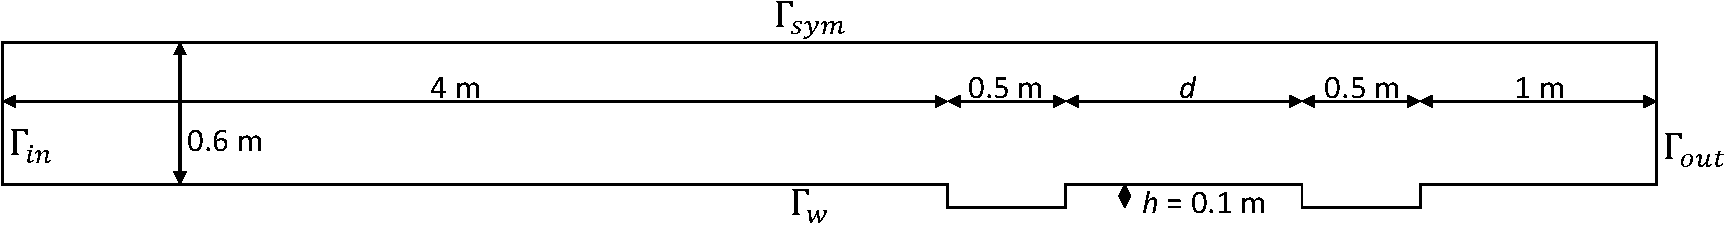
\includegraphics[width=\textwidth]{cavities_domain.pdf}
%\end{figure}
%\begin{figure}
%	\centering
%	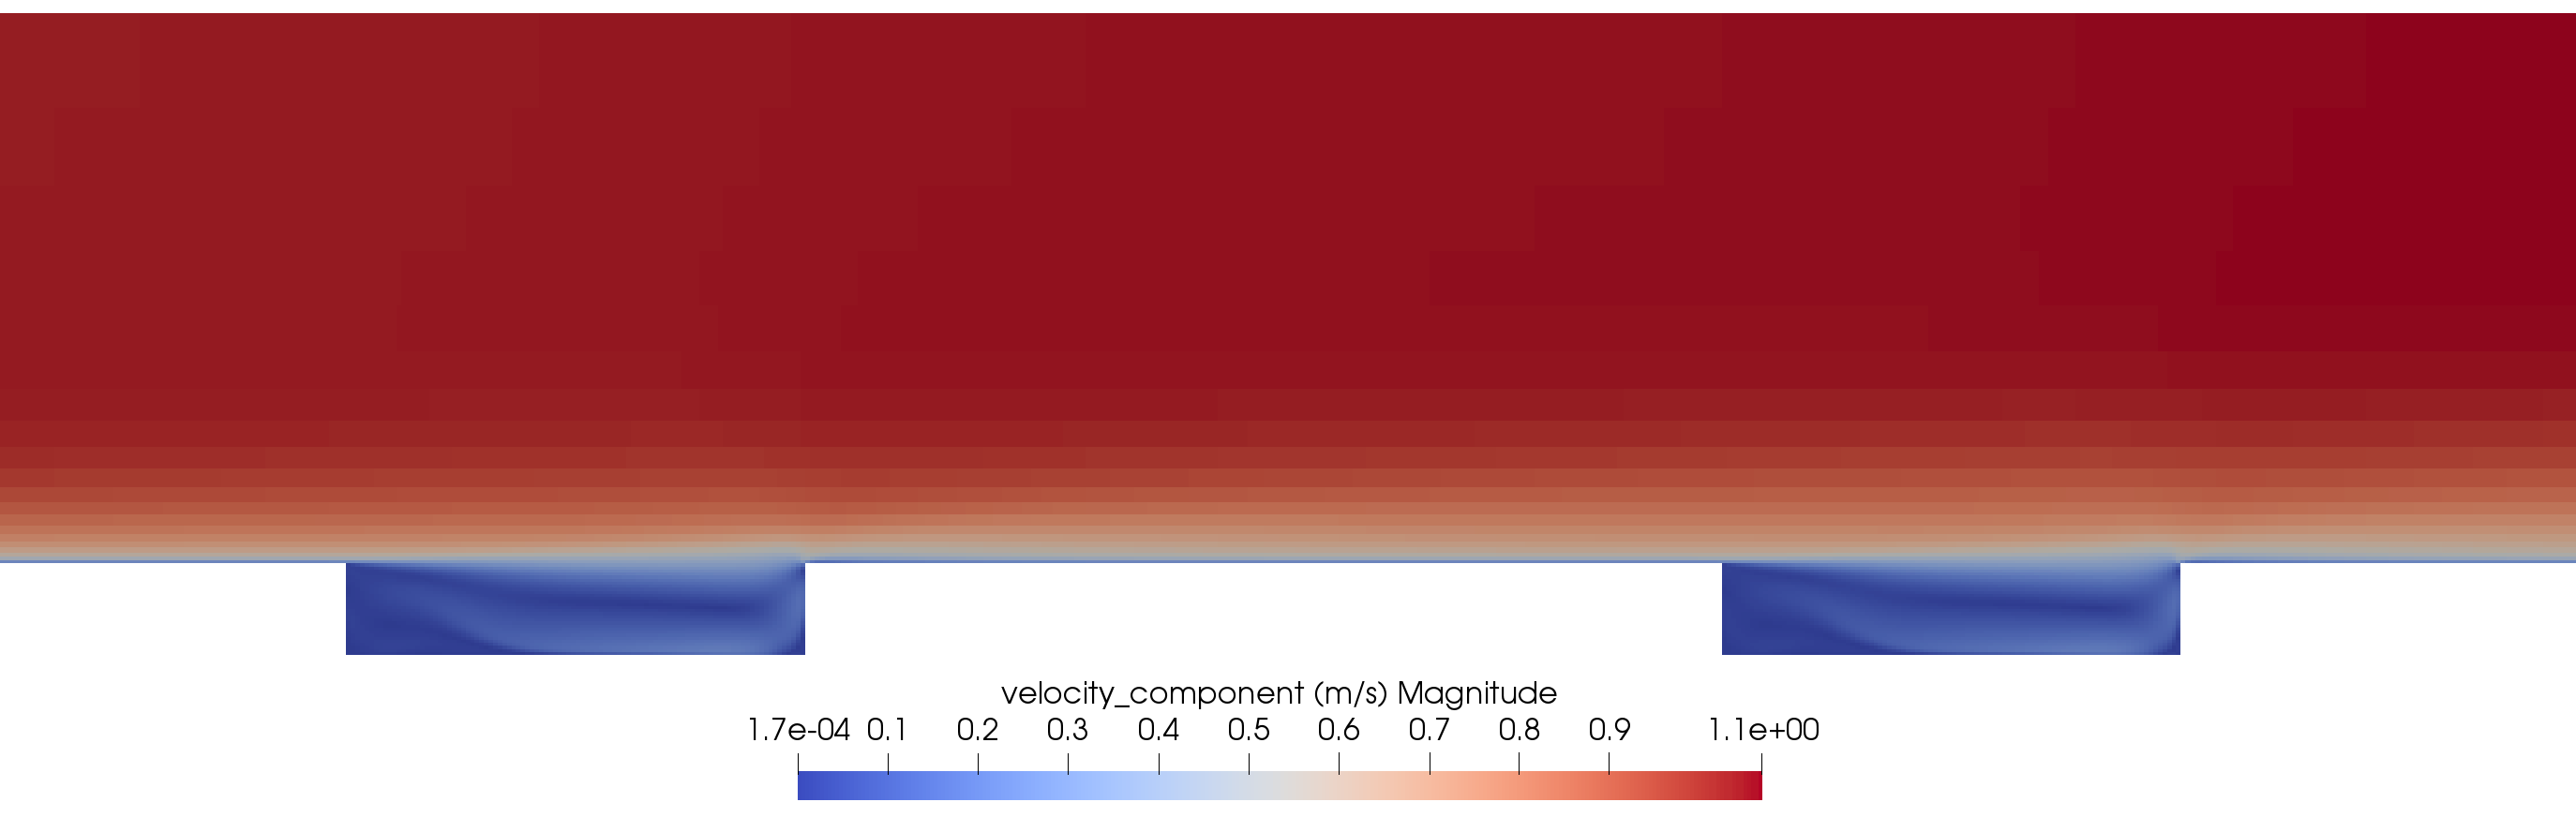
\includegraphics[width=\textwidth, trim={0 0 0 6cm}, 
%	clip]{cavities_dist1_vel.png}
%\end{figure}
%\begin{itemize}
%	\item $Re = 60000$.
%	\item $d$ ranging from $\SI{0.05}{m}$ to $\SI{2}{m}$.
%\end{itemize}
%\end{frame}
%%%%%%%%%%%%%%%%%%%%%%%%%%%%%%%%%%%%%%%%%%%%%%%%%%%%%%%%%%%%%%%%%%%%%%%%%%
%\begin{frame}{Cavities}
%\begin{figure}
%	\centering
%	\subfloat[\scriptsize $u$ profile at $y=h$, 
%	$d=\SI{1}{m}$]{\hspace{-0.5cm}% This file was created by matlab2tikz.
%
\definecolor{mycolor1}{rgb}{0.00000,0.44700,0.74100}%
%
\begin{tikzpicture}

\begin{axis}[%
width=0.951\figwidth,
height=0.75\cavheight,
at={(0\figwidth,0\cavheight)},
scale only axis,
xmin=3.5,
xmax=7,
xlabel style={font=\color{white!15!black}},
xlabel={$x$ [m]},
ymin=0.15,
ymax=0.4,
ylabel style={font=\color{white!15!black}},
ylabel={$u$ [m/s]},
axis background/.style={fill=white},
xmajorgrids,
ymajorgrids
]
\addplot [color=mycolor1, line width=1.0pt, forget plot]
  table[row sep=crcr]{%
3.505	0.262676\\
3.51	0.262616\\
3.515	0.262616\\
3.52	0.262616\\
3.525	0.262616\\
3.53	0.262616\\
3.535	0.262616\\
3.54	0.262616\\
3.545	0.262616\\
3.55	0.262616\\
3.555	0.262616\\
3.56	0.262558\\
3.565	0.262558\\
3.57	0.262558\\
3.575	0.262558\\
3.58	0.262558\\
3.585	0.262558\\
3.59	0.262558\\
3.595	0.262558\\
3.6	0.262558\\
3.605	0.262503\\
3.61	0.262503\\
3.615	0.262503\\
3.62	0.262503\\
3.625	0.262503\\
3.63	0.262503\\
3.635	0.262503\\
3.64	0.262503\\
3.645	0.26245\\
3.65	0.26245\\
3.655	0.26245\\
3.66	0.26245\\
3.665	0.26245\\
3.67	0.26245\\
3.675	0.26245\\
3.68	0.26245\\
3.685	0.262399\\
3.69	0.262399\\
3.695	0.262399\\
3.7	0.262399\\
3.705	0.262399\\
3.71	0.262399\\
3.715	0.262399\\
3.72	0.262351\\
3.725	0.262351\\
3.73	0.262351\\
3.735	0.262351\\
3.74	0.262351\\
3.745	0.262351\\
3.75	0.262306\\
3.755	0.262306\\
3.76	0.262306\\
3.765	0.262306\\
3.77	0.262306\\
3.775	0.262265\\
3.78	0.262265\\
3.785	0.262265\\
3.79	0.262265\\
3.795	0.262265\\
3.8	0.262227\\
3.805	0.262227\\
3.81	0.262227\\
3.815	0.262227\\
3.82	0.262227\\
3.825	0.262195\\
3.83	0.262195\\
3.835	0.262195\\
3.84	0.262195\\
3.845	0.262168\\
3.85	0.262168\\
3.855	0.262168\\
3.86	0.262168\\
3.865	0.262148\\
3.87	0.262148\\
3.875	0.262148\\
3.88	0.262148\\
3.885	0.262137\\
3.89	0.262137\\
3.895	0.262137\\
3.9	0.262135\\
3.905	0.262135\\
3.91	0.262135\\
3.915	0.262145\\
3.92	0.262145\\
3.925	0.262168\\
3.93	0.262168\\
3.935	0.262168\\
3.94	0.262209\\
3.945	0.262209\\
3.95	0.262272\\
3.955	0.262272\\
3.96	0.262368\\
3.965	0.262368\\
3.97	0.262512\\
3.975	0.262728\\
3.98	0.262728\\
3.985	0.263067\\
3.99	0.263662\\
3.995	0.26509\\
4	0.268628\\
4.005	0.268628\\
4.01	0.27414\\
4.015	0.280032\\
4.02	0.285537\\
4.025	0.290514\\
4.03	0.294956\\
4.035	0.298941\\
4.04	0.302551\\
4.045	0.305844\\
4.05	0.308863\\
4.055	0.311641\\
4.06	0.314202\\
4.065	0.316568\\
4.07	0.318763\\
4.075	0.320816\\
4.08	0.322754\\
4.085	0.324599\\
4.09	0.326371\\
4.095	0.328094\\
4.1	0.329791\\
4.105	0.331472\\
4.11	0.333147\\
4.115	0.334828\\
4.12	0.33652\\
4.125	0.33823\\
4.13	0.339963\\
4.135	0.341723\\
4.14	0.343509\\
4.145	0.345319\\
4.15	0.347147\\
4.155	0.348985\\
4.16	0.350827\\
4.165	0.352663\\
4.17	0.354484\\
4.175	0.356285\\
4.18	0.358057\\
4.185	0.359792\\
4.19	0.361487\\
4.195	0.363137\\
4.2	0.364737\\
4.205	0.366281\\
4.21	0.367768\\
4.215	0.369193\\
4.22	0.370556\\
4.225	0.371852\\
4.23	0.373082\\
4.235	0.374244\\
4.24	0.375337\\
4.245	0.376361\\
4.25	0.377316\\
4.255	0.378202\\
4.26	0.37902\\
4.265	0.379771\\
4.27	0.380456\\
4.275	0.381076\\
4.28	0.381633\\
4.285	0.38213\\
4.29	0.382567\\
4.295	0.382947\\
4.3	0.383274\\
4.305	0.383549\\
4.31	0.383777\\
4.315	0.38396\\
4.32	0.384103\\
4.325	0.384211\\
4.33	0.384287\\
4.335	0.384334\\
4.34	0.384355\\
4.345	0.384354\\
4.35	0.384333\\
4.355	0.384293\\
4.36	0.384235\\
4.365	0.38416\\
4.37	0.384064\\
4.375	0.383945\\
4.38	0.383796\\
4.385	0.383606\\
4.39	0.383366\\
4.395	0.383059\\
4.4	0.382666\\
4.405	0.382164\\
4.41	0.381524\\
4.415	0.380707\\
4.42	0.379663\\
4.425	0.378339\\
4.43	0.376682\\
4.435	0.374643\\
4.44	0.372186\\
4.445	0.369265\\
4.45	0.365813\\
4.455	0.361743\\
4.46	0.356928\\
4.465	0.351207\\
4.47	0.344355\\
4.475	0.336065\\
4.48	0.325962\\
4.485	0.313661\\
4.49	0.298724\\
4.495	0.282999\\
4.5	0.295616\\
4.505	0.264581\\
4.51	0.193707\\
4.515	0.16835\\
4.52	0.163515\\
4.525	0.167251\\
4.53	0.173801\\
4.535	0.181008\\
4.54	0.188012\\
4.545	0.194581\\
4.55	0.194581\\
4.555	0.200482\\
4.56	0.205777\\
4.565	0.210593\\
4.57	0.210593\\
4.575	0.214974\\
4.58	0.218972\\
4.585	0.222644\\
4.59	0.222644\\
4.595	0.226024\\
4.6	0.229138\\
4.605	0.229138\\
4.61	0.232011\\
4.615	0.234665\\
4.62	0.234665\\
4.625	0.237118\\
4.63	0.237118\\
4.635	0.239386\\
4.64	0.241484\\
4.645	0.241484\\
4.65	0.243426\\
4.655	0.243426\\
4.66	0.245225\\
4.665	0.245225\\
4.67	0.24689\\
4.675	0.24689\\
4.68	0.248431\\
4.685	0.249852\\
4.69	0.249852\\
4.695	0.251162\\
4.7	0.251162\\
4.705	0.252364\\
4.71	0.252364\\
4.715	0.253465\\
4.72	0.253465\\
4.725	0.253465\\
4.73	0.25447\\
4.735	0.25447\\
4.74	0.255385\\
4.745	0.255385\\
4.75	0.256216\\
4.755	0.256216\\
4.76	0.256971\\
4.765	0.256971\\
4.77	0.257656\\
4.775	0.257656\\
4.78	0.257656\\
4.785	0.258274\\
4.79	0.258274\\
4.795	0.258831\\
4.8	0.258831\\
4.805	0.258831\\
4.81	0.25933\\
4.815	0.25933\\
4.82	0.259773\\
4.825	0.259773\\
4.83	0.259773\\
4.835	0.260165\\
4.84	0.260165\\
4.845	0.260165\\
4.85	0.260507\\
4.855	0.260507\\
4.86	0.260804\\
4.865	0.260804\\
4.87	0.260804\\
4.875	0.261058\\
4.88	0.261058\\
4.885	0.261058\\
4.89	0.261272\\
4.895	0.261272\\
4.9	0.261272\\
4.905	0.26145\\
4.91	0.26145\\
4.915	0.26145\\
4.92	0.261597\\
4.925	0.261597\\
4.93	0.261597\\
4.935	0.261716\\
4.94	0.261716\\
4.945	0.261716\\
4.95	0.26181\\
4.955	0.26181\\
4.96	0.26181\\
4.965	0.26181\\
4.97	0.261883\\
4.975	0.261883\\
4.98	0.261883\\
4.985	0.26194\\
4.99	0.26194\\
4.995	0.26194\\
5	0.26194\\
5.005	0.261979\\
5.01	0.261979\\
5.015	0.261979\\
5.02	0.261996\\
5.025	0.261996\\
5.03	0.261996\\
5.035	0.261995\\
5.04	0.261995\\
5.045	0.261995\\
5.05	0.261995\\
5.055	0.261983\\
5.06	0.261983\\
5.065	0.261983\\
5.07	0.261961\\
5.075	0.261961\\
5.08	0.261961\\
5.085	0.26193\\
5.09	0.26193\\
5.095	0.26193\\
5.1	0.261892\\
5.105	0.261892\\
5.11	0.261892\\
5.115	0.26185\\
5.12	0.26185\\
5.125	0.26185\\
5.13	0.261804\\
5.135	0.261804\\
5.14	0.261804\\
5.145	0.261757\\
5.15	0.261757\\
5.155	0.261709\\
5.16	0.261709\\
5.165	0.261709\\
5.17	0.261661\\
5.175	0.261661\\
5.18	0.261661\\
5.185	0.261614\\
5.19	0.261614\\
5.195	0.261568\\
5.2	0.261568\\
5.205	0.261568\\
5.21	0.261522\\
5.215	0.261522\\
5.22	0.261476\\
5.225	0.261476\\
5.23	0.261476\\
5.235	0.261432\\
5.24	0.261432\\
5.245	0.261388\\
5.25	0.261388\\
5.255	0.261344\\
5.26	0.261344\\
5.265	0.261302\\
5.27	0.261302\\
5.275	0.26126\\
5.28	0.26126\\
5.285	0.26126\\
5.29	0.261219\\
5.295	0.261219\\
5.3	0.261179\\
5.305	0.261179\\
5.31	0.261141\\
5.315	0.261141\\
5.32	0.261103\\
5.325	0.261067\\
5.33	0.261067\\
5.335	0.261032\\
5.34	0.261032\\
5.345	0.260999\\
5.35	0.260999\\
5.355	0.260967\\
5.36	0.260967\\
5.365	0.260937\\
5.37	0.26091\\
5.375	0.26091\\
5.38	0.260884\\
5.385	0.260884\\
5.39	0.260861\\
5.395	0.260841\\
5.4	0.260841\\
5.405	0.260825\\
5.41	0.260813\\
5.415	0.260813\\
5.42	0.260805\\
5.425	0.260803\\
5.43	0.260807\\
5.435	0.260807\\
5.44	0.260818\\
5.445	0.260838\\
5.45	0.260869\\
5.455	0.260869\\
5.46	0.260914\\
5.465	0.260979\\
5.47	0.261071\\
5.475	0.261202\\
5.48	0.261396\\
5.485	0.261698\\
5.49	0.262222\\
5.495	0.26347\\
5.5	0.266629\\
5.505	0.266629\\
5.51	0.271595\\
5.515	0.276913\\
5.52	0.281899\\
5.525	0.28642\\
5.53	0.290467\\
5.535	0.294107\\
5.54	0.297413\\
5.545	0.300435\\
5.55	0.303213\\
5.555	0.305775\\
5.56	0.30814\\
5.565	0.310327\\
5.57	0.312362\\
5.575	0.314269\\
5.58	0.316073\\
5.585	0.317791\\
5.59	0.319442\\
5.595	0.321042\\
5.6	0.322609\\
5.605	0.324163\\
5.61	0.325711\\
5.615	0.327261\\
5.62	0.328822\\
5.625	0.330398\\
5.63	0.331996\\
5.635	0.333617\\
5.64	0.335264\\
5.645	0.336936\\
5.65	0.338634\\
5.655	0.340354\\
5.66	0.342088\\
5.665	0.34383\\
5.67	0.345572\\
5.675	0.347305\\
5.68	0.349021\\
5.685	0.350713\\
5.69	0.352373\\
5.695	0.353994\\
5.7	0.355573\\
5.705	0.357103\\
5.71	0.358579\\
5.715	0.36\\
5.72	0.361363\\
5.725	0.362667\\
5.73	0.363909\\
5.735	0.365089\\
5.74	0.366205\\
5.745	0.367258\\
5.75	0.368245\\
5.755	0.369167\\
5.76	0.370024\\
5.765	0.370815\\
5.77	0.371541\\
5.775	0.372204\\
5.78	0.372803\\
5.785	0.373342\\
5.79	0.37382\\
5.795	0.374241\\
5.8	0.374607\\
5.805	0.374921\\
5.81	0.375186\\
5.815	0.375404\\
5.82	0.375579\\
5.825	0.375716\\
5.83	0.375816\\
5.835	0.375883\\
5.84	0.375918\\
5.845	0.375925\\
5.85	0.375907\\
5.855	0.375866\\
5.86	0.3758\\
5.865	0.375709\\
5.87	0.37559\\
5.875	0.375439\\
5.88	0.375247\\
5.885	0.375009\\
5.89	0.374712\\
5.895	0.374345\\
5.9	0.373886\\
5.905	0.37331\\
5.91	0.372592\\
5.915	0.371699\\
5.92	0.370589\\
5.925	0.369218\\
5.93	0.367541\\
5.935	0.365513\\
5.94	0.363089\\
5.945	0.36021\\
5.95	0.356812\\
5.955	0.352805\\
5.96	0.348069\\
5.965	0.342443\\
5.97	0.335705\\
5.975	0.327557\\
5.98	0.317633\\
5.985	0.305563\\
5.99	0.290921\\
5.995	0.275548\\
6	0.288264\\
6.005	0.189663\\
6.01	0.189663\\
6.015	0.164357\\
6.02	0.160921\\
6.025	0.167072\\
6.03	0.167072\\
6.035	0.176188\\
6.04	0.185964\\
6.045	0.185964\\
6.05	0.195421\\
6.055	0.195421\\
6.06	0.203955\\
6.065	0.203955\\
6.07	0.211669\\
6.075	0.211669\\
6.08	0.21859\\
6.085	0.21859\\
6.09	0.21859\\
6.095	0.224818\\
6.1	0.224818\\
6.105	0.224818\\
6.11	0.230405\\
6.115	0.230405\\
6.12	0.230405\\
6.125	0.23541\\
6.13	0.23541\\
6.135	0.23541\\
6.14	0.239845\\
6.145	0.239845\\
6.15	0.239845\\
6.155	0.239845\\
6.16	0.24374\\
6.165	0.24374\\
6.17	0.24374\\
6.175	0.24374\\
6.18	0.24713\\
6.185	0.24713\\
6.19	0.24713\\
6.195	0.24713\\
6.2	0.24713\\
6.205	0.250021\\
6.21	0.250021\\
6.215	0.250021\\
6.22	0.250021\\
6.225	0.250021\\
6.23	0.252439\\
6.235	0.252439\\
6.24	0.252439\\
6.245	0.252439\\
6.25	0.252439\\
6.255	0.254431\\
6.26	0.254431\\
6.265	0.254431\\
6.27	0.254431\\
6.275	0.254431\\
6.28	0.254431\\
6.285	0.256028\\
6.29	0.256028\\
6.295	0.256028\\
6.3	0.256028\\
6.305	0.256028\\
6.31	0.256028\\
6.315	0.256028\\
6.32	0.257261\\
6.325	0.257261\\
6.33	0.257261\\
6.335	0.257261\\
6.34	0.257261\\
6.345	0.257261\\
6.35	0.257261\\
6.355	0.257261\\
6.36	0.258168\\
6.365	0.258168\\
6.37	0.258168\\
6.375	0.258168\\
6.38	0.258168\\
6.385	0.258168\\
6.39	0.258168\\
6.395	0.258168\\
6.4	0.258804\\
6.405	0.258804\\
6.41	0.258804\\
6.415	0.258804\\
6.42	0.258804\\
6.425	0.258804\\
6.43	0.258804\\
6.435	0.258804\\
6.44	0.258804\\
6.445	0.259215\\
6.45	0.259215\\
6.455	0.259215\\
6.46	0.259215\\
6.465	0.259215\\
6.47	0.259215\\
6.475	0.259215\\
6.48	0.259215\\
6.485	0.259215\\
6.49	0.259449\\
6.495	0.259449\\
6.5	0.259449\\
6.505	0.259449\\
6.51	0.259449\\
6.515	0.259449\\
6.52	0.259449\\
6.525	0.259449\\
6.53	0.259449\\
6.535	0.259449\\
6.54	0.259449\\
6.545	0.25952\\
6.55	0.25952\\
6.555	0.25952\\
6.56	0.25952\\
6.565	0.25952\\
6.57	0.25952\\
6.575	0.25952\\
6.58	0.25952\\
6.585	0.25952\\
6.59	0.25952\\
6.595	0.25952\\
6.6	0.25952\\
6.605	0.259476\\
6.61	0.259476\\
6.615	0.259476\\
6.62	0.259476\\
6.625	0.259476\\
6.63	0.259476\\
6.635	0.259476\\
6.64	0.259476\\
6.645	0.259476\\
6.65	0.259476\\
6.655	0.259476\\
6.66	0.259476\\
6.665	0.259476\\
6.67	0.259376\\
6.675	0.259376\\
6.68	0.259376\\
6.685	0.259376\\
6.69	0.259376\\
6.695	0.259376\\
6.7	0.259376\\
6.705	0.259376\\
6.71	0.259376\\
6.715	0.259376\\
6.72	0.259376\\
6.725	0.259376\\
6.73	0.259376\\
6.735	0.259376\\
6.74	0.259219\\
6.745	0.259219\\
6.75	0.259219\\
6.755	0.259219\\
6.76	0.259219\\
6.765	0.259219\\
6.77	0.259219\\
6.775	0.259219\\
6.78	0.259219\\
6.785	0.259219\\
6.79	0.259219\\
6.795	0.259219\\
6.8	0.259219\\
6.805	0.259219\\
6.81	0.259219\\
6.815	0.259219\\
6.82	0.25916\\
6.825	0.25916\\
6.83	0.25916\\
6.835	0.25916\\
6.84	0.25916\\
6.845	0.25916\\
6.85	0.25916\\
6.855	0.25916\\
6.86	0.25916\\
6.865	0.25916\\
6.87	0.25916\\
6.875	0.25916\\
6.88	0.25916\\
6.885	0.25916\\
6.89	0.25916\\
6.895	0.25916\\
6.9	0.25916\\
6.905	0.259157\\
6.91	0.259157\\
6.915	0.259157\\
6.92	0.259157\\
6.925	0.259157\\
6.93	0.259157\\
6.935	0.259157\\
6.94	0.259157\\
6.945	0.259157\\
6.95	0.259157\\
6.955	0.259157\\
6.96	0.259157\\
6.965	0.259157\\
6.97	0.259157\\
6.975	0.259157\\
6.98	0.259157\\
6.985	0.259157\\
6.99	0.259157\\
6.995	0.259157\\
7	0.259157\\
};
\end{axis}
\end{tikzpicture}%}
%	\subfloat[\scriptsize Peak velocity above the second 
%	cavity]{% This file was created by matlab2tikz.
%
\definecolor{mycolor1}{rgb}{0.00000,0.44700,0.74100}%
%
\begin{tikzpicture}

\begin{axis}[%
width=0.951\figwidth,
height=0.75\cavheight,
at={(0\figwidth,0\cavheight)},
scale only axis,
xmin=0,
xmax=2,
xlabel={$d$ [m]},
ymin=0.35,
ymax=0.38,
ylabel={velocity [m/s]},
axis background/.style={fill=white},
xmajorgrids,
ymajorgrids,
yticklabel style={/pgf/number format/.cd,fixed,precision=3}
]
\addplot [color=mycolor1, line width=1.0pt, mark size=2.5pt, mark=o, mark options={solid, mycolor1}, forget plot]
  table[row sep=crcr]
%\end{figure}
%\end{frame}
%%%%%%%%%%%%%%%%%%%%%%%%%%%%%%%%%%%%%%%%%%%%%%%%%%%%%%%%%%%%%%%%%%%%%%%%%%%
\begin{frame}{Coupled problem with shallow cavities}
\begin{figure}
	\centering
	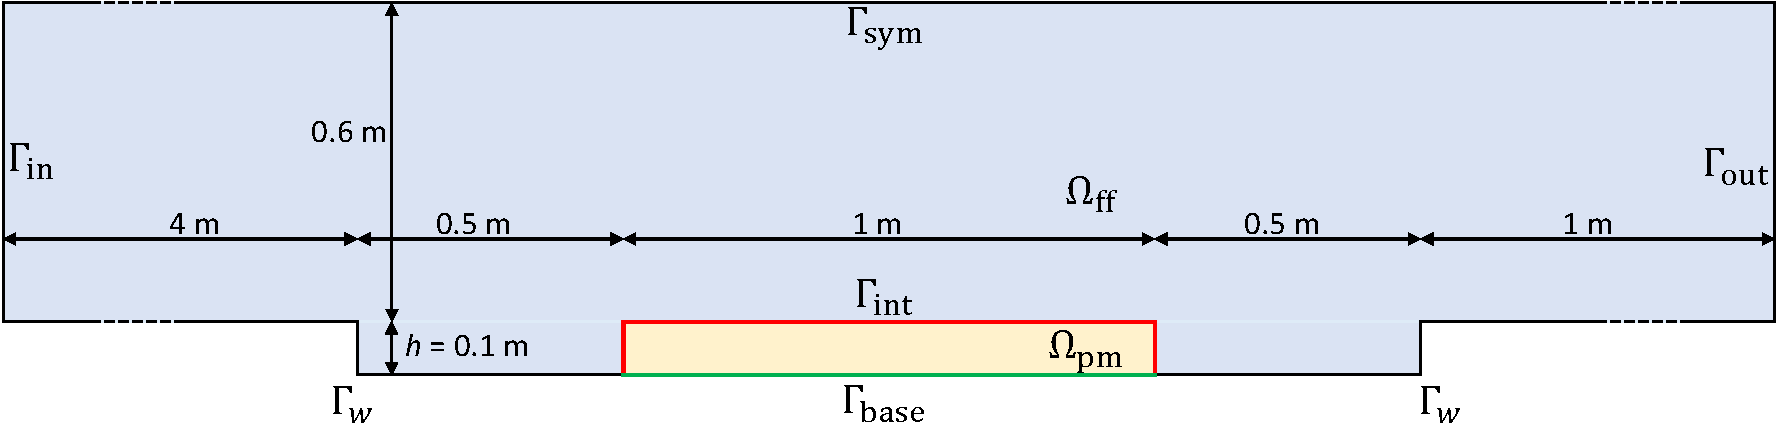
\includegraphics[width=\textwidth]{cavities_multidomain_slides.pdf}
\end{figure}
Flow in a channel with two shallow cavities on the lower boundary and a porous-medium 
between them.
\begin{itemize}
	\item $Re=60000$.
	\item Permeability ranging from $\SI{3.1e-12}{m^2}$ to $\SI{3.1e-6}{m^2}$.
	\item $\alpha_\text{BJ} = 2$, $C_F=0.55$.
\end{itemize}
\end{frame}
%%%%%%%%%%%%%%%%%%%%%%%%%%%%%%%%%%%%%%%%%%%%%%%%%%%%%%%%%%%%%%%%%%%%%%%%
\begin{frame}{Coupled problem with shallow cavities}
\begin{figure}
	\centering
	\hspace{-0.5cm}
	% This file was created by matlab2tikz.
%
\definecolor{mycolor1}{rgb}{0.00000,0.44700,0.74100}%
\definecolor{mycolor2}{rgb}{0.85000,0.32500,0.09800}%
\definecolor{mycolor3}{rgb}{0.92900,0.69400,0.12500}%
\definecolor{mycolor4}{rgb}{0.49400,0.18400,0.55600}%
\definecolor{mycolor5}{rgb}{0.46600,0.67400,0.18800}%
\definecolor{mycolor6}{rgb}{0.30100,0.74500,0.93300}%
\definecolor{mycolor7}{rgb}{0.63500,0.07800,0.18400}%
%
\begin{tikzpicture}

\begin{axis}[%
width=0.951\bfswidth,
height=0.75\roughheight,
at={(0\bfswidth,0\roughheight)},
scale only axis,
xmin=3.5,
xmax=7,
xlabel={$x$ [m]},
ymin=0,
ymax=0.45,
ylabel={$u$ [m/s]},
axis background/.style={fill=white},
xmajorgrids,
ymajorgrids,
legend style={at={(0.01,0.02)}, anchor=south west, legend cell align=left, align=left, font=\tiny}
]
\addplot [color=mycolor1, line width=1.0pt]
  table[row sep=crcr]{%
3.505	0.262676\\
3.51	0.262616\\
3.515	0.262616\\
3.52	0.262616\\
3.525	0.262616\\
3.53	0.262616\\
3.535	0.262616\\
3.54	0.262616\\
3.545	0.262616\\
3.55	0.262616\\
3.555	0.262616\\
3.56	0.262558\\
3.565	0.262558\\
3.57	0.262558\\
3.575	0.262558\\
3.58	0.262558\\
3.585	0.262558\\
3.59	0.262558\\
3.595	0.262558\\
3.6	0.262558\\
3.605	0.262503\\
3.61	0.262503\\
3.615	0.262503\\
3.62	0.262503\\
3.625	0.262503\\
3.63	0.262503\\
3.635	0.262503\\
3.64	0.262503\\
3.645	0.26245\\
3.65	0.26245\\
3.655	0.26245\\
3.66	0.26245\\
3.665	0.26245\\
3.67	0.26245\\
3.675	0.26245\\
3.68	0.26245\\
3.685	0.262399\\
3.69	0.262399\\
3.695	0.262399\\
3.7	0.262399\\
3.705	0.262399\\
3.71	0.262399\\
3.715	0.262399\\
3.72	0.262351\\
3.725	0.262351\\
3.73	0.262351\\
3.735	0.262351\\
3.74	0.262351\\
3.745	0.262351\\
3.75	0.262306\\
3.755	0.262306\\
3.76	0.262306\\
3.765	0.262306\\
3.77	0.262306\\
3.775	0.262265\\
3.78	0.262265\\
3.785	0.262265\\
3.79	0.262265\\
3.795	0.262265\\
3.8	0.262227\\
3.805	0.262227\\
3.81	0.262227\\
3.815	0.262227\\
3.82	0.262227\\
3.825	0.262195\\
3.83	0.262195\\
3.835	0.262195\\
3.84	0.262195\\
3.845	0.262168\\
3.85	0.262168\\
3.855	0.262168\\
3.86	0.262168\\
3.865	0.262148\\
3.87	0.262148\\
3.875	0.262148\\
3.88	0.262148\\
3.885	0.262137\\
3.89	0.262137\\
3.895	0.262137\\
3.9	0.262135\\
3.905	0.262135\\
3.91	0.262135\\
3.915	0.262145\\
3.92	0.262145\\
3.925	0.262168\\
3.93	0.262168\\
3.935	0.262168\\
3.94	0.262209\\
3.945	0.262209\\
3.95	0.262272\\
3.955	0.262272\\
3.96	0.262368\\
3.965	0.262368\\
3.97	0.262512\\
3.975	0.262728\\
3.98	0.262728\\
3.985	0.263067\\
3.99	0.263662\\
3.995	0.26509\\
4	0.268628\\
4.005	0.268628\\
4.01	0.27414\\
4.015	0.280032\\
4.02	0.285537\\
4.025	0.290514\\
4.03	0.294956\\
4.035	0.298941\\
4.04	0.302551\\
4.045	0.305844\\
4.05	0.308863\\
4.055	0.311641\\
4.06	0.314202\\
4.065	0.316568\\
4.07	0.318763\\
4.075	0.320816\\
4.08	0.322754\\
4.085	0.324599\\
4.09	0.326371\\
4.095	0.328094\\
4.1	0.329791\\
4.105	0.331472\\
4.11	0.333147\\
4.115	0.334828\\
4.12	0.33652\\
4.125	0.33823\\
4.13	0.339963\\
4.135	0.341723\\
4.14	0.343509\\
4.145	0.345319\\
4.15	0.347147\\
4.155	0.348985\\
4.16	0.350827\\
4.165	0.352663\\
4.17	0.354484\\
4.175	0.356285\\
4.18	0.358057\\
4.185	0.359792\\
4.19	0.361487\\
4.195	0.363137\\
4.2	0.364737\\
4.205	0.366281\\
4.21	0.367768\\
4.215	0.369193\\
4.22	0.370556\\
4.225	0.371852\\
4.23	0.373082\\
4.235	0.374244\\
4.24	0.375337\\
4.245	0.376361\\
4.25	0.377316\\
4.255	0.378202\\
4.26	0.37902\\
4.265	0.379771\\
4.27	0.380456\\
4.275	0.381076\\
4.28	0.381633\\
4.285	0.38213\\
4.29	0.382567\\
4.295	0.382947\\
4.3	0.383274\\
4.305	0.383549\\
4.31	0.383777\\
4.315	0.38396\\
4.32	0.384103\\
4.325	0.384211\\
4.33	0.384287\\
4.335	0.384334\\
4.34	0.384355\\
4.345	0.384354\\
4.35	0.384333\\
4.355	0.384293\\
4.36	0.384235\\
4.365	0.38416\\
4.37	0.384064\\
4.375	0.383945\\
4.38	0.383796\\
4.385	0.383606\\
4.39	0.383366\\
4.395	0.383059\\
4.4	0.382666\\
4.405	0.382164\\
4.41	0.381524\\
4.415	0.380707\\
4.42	0.379663\\
4.425	0.378339\\
4.43	0.376682\\
4.435	0.374643\\
4.44	0.372186\\
4.445	0.369265\\
4.45	0.365813\\
4.455	0.361743\\
4.46	0.356928\\
4.465	0.351207\\
4.47	0.344355\\
4.475	0.336065\\
4.48	0.325962\\
4.485	0.313661\\
4.49	0.298724\\
4.495	0.282999\\
4.5	0.295616\\
4.505	0.264581\\
4.51	0.193707\\
4.515	0.16835\\
4.52	0.163515\\
4.525	0.167251\\
4.53	0.173801\\
4.535	0.181008\\
4.54	0.188012\\
4.545	0.194581\\
4.55	0.194581\\
4.555	0.200482\\
4.56	0.205777\\
4.565	0.210593\\
4.57	0.210593\\
4.575	0.214974\\
4.58	0.218972\\
4.585	0.222644\\
4.59	0.222644\\
4.595	0.226024\\
4.6	0.229138\\
4.605	0.229138\\
4.61	0.232011\\
4.615	0.234665\\
4.62	0.234665\\
4.625	0.237118\\
4.63	0.237118\\
4.635	0.239386\\
4.64	0.241484\\
4.645	0.241484\\
4.65	0.243426\\
4.655	0.243426\\
4.66	0.245225\\
4.665	0.245225\\
4.67	0.24689\\
4.675	0.24689\\
4.68	0.248431\\
4.685	0.249852\\
4.69	0.249852\\
4.695	0.251162\\
4.7	0.251162\\
4.705	0.252364\\
4.71	0.252364\\
4.715	0.253465\\
4.72	0.253465\\
4.725	0.253465\\
4.73	0.25447\\
4.735	0.25447\\
4.74	0.255385\\
4.745	0.255385\\
4.75	0.256216\\
4.755	0.256216\\
4.76	0.256971\\
4.765	0.256971\\
4.77	0.257656\\
4.775	0.257656\\
4.78	0.257656\\
4.785	0.258274\\
4.79	0.258274\\
4.795	0.258831\\
4.8	0.258831\\
4.805	0.258831\\
4.81	0.25933\\
4.815	0.25933\\
4.82	0.259773\\
4.825	0.259773\\
4.83	0.259773\\
4.835	0.260165\\
4.84	0.260165\\
4.845	0.260165\\
4.85	0.260507\\
4.855	0.260507\\
4.86	0.260804\\
4.865	0.260804\\
4.87	0.260804\\
4.875	0.261058\\
4.88	0.261058\\
4.885	0.261058\\
4.89	0.261272\\
4.895	0.261272\\
4.9	0.261272\\
4.905	0.26145\\
4.91	0.26145\\
4.915	0.26145\\
4.92	0.261597\\
4.925	0.261597\\
4.93	0.261597\\
4.935	0.261716\\
4.94	0.261716\\
4.945	0.261716\\
4.95	0.26181\\
4.955	0.26181\\
4.96	0.26181\\
4.965	0.26181\\
4.97	0.261883\\
4.975	0.261883\\
4.98	0.261883\\
4.985	0.26194\\
4.99	0.26194\\
4.995	0.26194\\
5	0.26194\\
5.005	0.261979\\
5.01	0.261979\\
5.015	0.261979\\
5.02	0.261996\\
5.025	0.261996\\
5.03	0.261996\\
5.035	0.261995\\
5.04	0.261995\\
5.045	0.261995\\
5.05	0.261995\\
5.055	0.261983\\
5.06	0.261983\\
5.065	0.261983\\
5.07	0.261961\\
5.075	0.261961\\
5.08	0.261961\\
5.085	0.26193\\
5.09	0.26193\\
5.095	0.26193\\
5.1	0.261892\\
5.105	0.261892\\
5.11	0.261892\\
5.115	0.26185\\
5.12	0.26185\\
5.125	0.26185\\
5.13	0.261804\\
5.135	0.261804\\
5.14	0.261804\\
5.145	0.261757\\
5.15	0.261757\\
5.155	0.261709\\
5.16	0.261709\\
5.165	0.261709\\
5.17	0.261661\\
5.175	0.261661\\
5.18	0.261661\\
5.185	0.261614\\
5.19	0.261614\\
5.195	0.261568\\
5.2	0.261568\\
5.205	0.261568\\
5.21	0.261522\\
5.215	0.261522\\
5.22	0.261476\\
5.225	0.261476\\
5.23	0.261476\\
5.235	0.261432\\
5.24	0.261432\\
5.245	0.261388\\
5.25	0.261388\\
5.255	0.261344\\
5.26	0.261344\\
5.265	0.261302\\
5.27	0.261302\\
5.275	0.26126\\
5.28	0.26126\\
5.285	0.26126\\
5.29	0.261219\\
5.295	0.261219\\
5.3	0.261179\\
5.305	0.261179\\
5.31	0.261141\\
5.315	0.261141\\
5.32	0.261103\\
5.325	0.261067\\
5.33	0.261067\\
5.335	0.261032\\
5.34	0.261032\\
5.345	0.260999\\
5.35	0.260999\\
5.355	0.260967\\
5.36	0.260967\\
5.365	0.260937\\
5.37	0.26091\\
5.375	0.26091\\
5.38	0.260884\\
5.385	0.260884\\
5.39	0.260861\\
5.395	0.260841\\
5.4	0.260841\\
5.405	0.260825\\
5.41	0.260813\\
5.415	0.260813\\
5.42	0.260805\\
5.425	0.260803\\
5.43	0.260807\\
5.435	0.260807\\
5.44	0.260818\\
5.445	0.260838\\
5.45	0.260869\\
5.455	0.260869\\
5.46	0.260914\\
5.465	0.260979\\
5.47	0.261071\\
5.475	0.261202\\
5.48	0.261396\\
5.485	0.261698\\
5.49	0.262222\\
5.495	0.26347\\
5.5	0.266629\\
5.505	0.266629\\
5.51	0.271595\\
5.515	0.276913\\
5.52	0.281899\\
5.525	0.28642\\
5.53	0.290467\\
5.535	0.294107\\
5.54	0.297413\\
5.545	0.300435\\
5.55	0.303213\\
5.555	0.305775\\
5.56	0.30814\\
5.565	0.310327\\
5.57	0.312362\\
5.575	0.314269\\
5.58	0.316073\\
5.585	0.317791\\
5.59	0.319442\\
5.595	0.321042\\
5.6	0.322609\\
5.605	0.324163\\
5.61	0.325711\\
5.615	0.327261\\
5.62	0.328822\\
5.625	0.330398\\
5.63	0.331996\\
5.635	0.333617\\
5.64	0.335264\\
5.645	0.336936\\
5.65	0.338634\\
5.655	0.340354\\
5.66	0.342088\\
5.665	0.34383\\
5.67	0.345572\\
5.675	0.347305\\
5.68	0.349021\\
5.685	0.350713\\
5.69	0.352373\\
5.695	0.353994\\
5.7	0.355573\\
5.705	0.357103\\
5.71	0.358579\\
5.715	0.36\\
5.72	0.361363\\
5.725	0.362667\\
5.73	0.363909\\
5.735	0.365089\\
5.74	0.366205\\
5.745	0.367258\\
5.75	0.368245\\
5.755	0.369167\\
5.76	0.370024\\
5.765	0.370815\\
5.77	0.371541\\
5.775	0.372204\\
5.78	0.372803\\
5.785	0.373342\\
5.79	0.37382\\
5.795	0.374241\\
5.8	0.374607\\
5.805	0.374921\\
5.81	0.375186\\
5.815	0.375404\\
5.82	0.375579\\
5.825	0.375716\\
5.83	0.375816\\
5.835	0.375883\\
5.84	0.375918\\
5.845	0.375925\\
5.85	0.375907\\
5.855	0.375866\\
5.86	0.3758\\
5.865	0.375709\\
5.87	0.37559\\
5.875	0.375439\\
5.88	0.375247\\
5.885	0.375009\\
5.89	0.374712\\
5.895	0.374345\\
5.9	0.373886\\
5.905	0.37331\\
5.91	0.372592\\
5.915	0.371699\\
5.92	0.370589\\
5.925	0.369218\\
5.93	0.367541\\
5.935	0.365513\\
5.94	0.363089\\
5.945	0.36021\\
5.95	0.356812\\
5.955	0.352805\\
5.96	0.348069\\
5.965	0.342443\\
5.97	0.335705\\
5.975	0.327557\\
5.98	0.317633\\
5.985	0.305563\\
5.99	0.290921\\
5.995	0.275548\\
6	0.288264\\
6.005	0.189663\\
6.01	0.189663\\
6.015	0.164357\\
6.02	0.160921\\
6.025	0.167072\\
6.03	0.167072\\
6.035	0.176188\\
6.04	0.185964\\
6.045	0.185964\\
6.05	0.195421\\
6.055	0.195421\\
6.06	0.203955\\
6.065	0.203955\\
6.07	0.211669\\
6.075	0.211669\\
6.08	0.21859\\
6.085	0.21859\\
6.09	0.21859\\
6.095	0.224818\\
6.1	0.224818\\
6.105	0.224818\\
6.11	0.230405\\
6.115	0.230405\\
6.12	0.230405\\
6.125	0.23541\\
6.13	0.23541\\
6.135	0.23541\\
6.14	0.239845\\
6.145	0.239845\\
6.15	0.239845\\
6.155	0.239845\\
6.16	0.24374\\
6.165	0.24374\\
6.17	0.24374\\
6.175	0.24374\\
6.18	0.24713\\
6.185	0.24713\\
6.19	0.24713\\
6.195	0.24713\\
6.2	0.24713\\
6.205	0.250021\\
6.21	0.250021\\
6.215	0.250021\\
6.22	0.250021\\
6.225	0.250021\\
6.23	0.252439\\
6.235	0.252439\\
6.24	0.252439\\
6.245	0.252439\\
6.25	0.252439\\
6.255	0.254431\\
6.26	0.254431\\
6.265	0.254431\\
6.27	0.254431\\
6.275	0.254431\\
6.28	0.254431\\
6.285	0.256028\\
6.29	0.256028\\
6.295	0.256028\\
6.3	0.256028\\
6.305	0.256028\\
6.31	0.256028\\
6.315	0.256028\\
6.32	0.257261\\
6.325	0.257261\\
6.33	0.257261\\
6.335	0.257261\\
6.34	0.257261\\
6.345	0.257261\\
6.35	0.257261\\
6.355	0.257261\\
6.36	0.258168\\
6.365	0.258168\\
6.37	0.258168\\
6.375	0.258168\\
6.38	0.258168\\
6.385	0.258168\\
6.39	0.258168\\
6.395	0.258168\\
6.4	0.258804\\
6.405	0.258804\\
6.41	0.258804\\
6.415	0.258804\\
6.42	0.258804\\
6.425	0.258804\\
6.43	0.258804\\
6.435	0.258804\\
6.44	0.258804\\
6.445	0.259215\\
6.45	0.259215\\
6.455	0.259215\\
6.46	0.259215\\
6.465	0.259215\\
6.47	0.259215\\
6.475	0.259215\\
6.48	0.259215\\
6.485	0.259215\\
6.49	0.259449\\
6.495	0.259449\\
6.5	0.259449\\
6.505	0.259449\\
6.51	0.259449\\
6.515	0.259449\\
6.52	0.259449\\
6.525	0.259449\\
6.53	0.259449\\
6.535	0.259449\\
6.54	0.259449\\
6.545	0.25952\\
6.55	0.25952\\
6.555	0.25952\\
6.56	0.25952\\
6.565	0.25952\\
6.57	0.25952\\
6.575	0.25952\\
6.58	0.25952\\
6.585	0.25952\\
6.59	0.25952\\
6.595	0.25952\\
6.6	0.25952\\
6.605	0.259476\\
6.61	0.259476\\
6.615	0.259476\\
6.62	0.259476\\
6.625	0.259476\\
6.63	0.259476\\
6.635	0.259476\\
6.64	0.259476\\
6.645	0.259476\\
6.65	0.259476\\
6.655	0.259476\\
6.66	0.259476\\
6.665	0.259476\\
6.67	0.259376\\
6.675	0.259376\\
6.68	0.259376\\
6.685	0.259376\\
6.69	0.259376\\
6.695	0.259376\\
6.7	0.259376\\
6.705	0.259376\\
6.71	0.259376\\
6.715	0.259376\\
6.72	0.259376\\
6.725	0.259376\\
6.73	0.259376\\
6.735	0.259376\\
6.74	0.259219\\
6.745	0.259219\\
6.75	0.259219\\
6.755	0.259219\\
6.76	0.259219\\
6.765	0.259219\\
6.77	0.259219\\
6.775	0.259219\\
6.78	0.259219\\
6.785	0.259219\\
6.79	0.259219\\
6.795	0.259219\\
6.8	0.259219\\
6.805	0.259219\\
6.81	0.259219\\
6.815	0.259219\\
6.82	0.25916\\
6.825	0.25916\\
6.83	0.25916\\
6.835	0.25916\\
6.84	0.25916\\
6.845	0.25916\\
6.85	0.25916\\
6.855	0.25916\\
6.86	0.25916\\
6.865	0.25916\\
6.87	0.25916\\
6.875	0.25916\\
6.88	0.25916\\
6.885	0.25916\\
6.89	0.25916\\
6.895	0.25916\\
6.9	0.25916\\
6.905	0.259157\\
6.91	0.259157\\
6.915	0.259157\\
6.92	0.259157\\
6.925	0.259157\\
6.93	0.259157\\
6.935	0.259157\\
6.94	0.259157\\
6.945	0.259157\\
6.95	0.259157\\
6.955	0.259157\\
6.96	0.259157\\
6.965	0.259157\\
6.97	0.259157\\
6.975	0.259157\\
6.98	0.259157\\
6.985	0.259157\\
6.99	0.259157\\
6.995	0.259157\\
7	0.259157\\
};
\addlegendentry{No pm}

\addplot [color=mycolor2, line width=1.0pt]
  table[row sep=crcr]{%
3.505	0.262676\\
3.51	0.262616\\
3.515	0.262616\\
3.52	0.262616\\
3.525	0.262616\\
3.53	0.262616\\
3.535	0.262616\\
3.54	0.262616\\
3.545	0.262616\\
3.55	0.262616\\
3.555	0.262616\\
3.56	0.262558\\
3.565	0.262558\\
3.57	0.262558\\
3.575	0.262558\\
3.58	0.262558\\
3.585	0.262558\\
3.59	0.262558\\
3.595	0.262558\\
3.6	0.262558\\
3.605	0.262503\\
3.61	0.262503\\
3.615	0.262503\\
3.62	0.262503\\
3.625	0.262503\\
3.63	0.262503\\
3.635	0.262503\\
3.64	0.262503\\
3.645	0.26245\\
3.65	0.26245\\
3.655	0.26245\\
3.66	0.26245\\
3.665	0.26245\\
3.67	0.26245\\
3.675	0.26245\\
3.68	0.26245\\
3.685	0.262399\\
3.69	0.262399\\
3.695	0.262399\\
3.7	0.262399\\
3.705	0.262399\\
3.71	0.262399\\
3.715	0.262399\\
3.72	0.262351\\
3.725	0.262351\\
3.73	0.262351\\
3.735	0.262351\\
3.74	0.262351\\
3.745	0.262351\\
3.75	0.262306\\
3.755	0.262306\\
3.76	0.262306\\
3.765	0.262306\\
3.77	0.262306\\
3.775	0.262265\\
3.78	0.262265\\
3.785	0.262265\\
3.79	0.262265\\
3.795	0.262265\\
3.8	0.262265\\
3.805	0.262227\\
3.81	0.262227\\
3.815	0.262227\\
3.82	0.262227\\
3.825	0.262195\\
3.83	0.262195\\
3.835	0.262195\\
3.84	0.262195\\
3.845	0.262168\\
3.85	0.262168\\
3.855	0.262168\\
3.86	0.262168\\
3.865	0.262148\\
3.87	0.262148\\
3.875	0.262148\\
3.88	0.262148\\
3.885	0.262136\\
3.89	0.262136\\
3.895	0.262136\\
3.9	0.262135\\
3.905	0.262135\\
3.91	0.262135\\
3.915	0.262145\\
3.92	0.262145\\
3.925	0.262168\\
3.93	0.262168\\
3.935	0.262168\\
3.94	0.262209\\
3.945	0.262209\\
3.95	0.262272\\
3.955	0.262272\\
3.96	0.262368\\
3.965	0.262368\\
3.97	0.262512\\
3.975	0.262727\\
3.98	0.262727\\
3.985	0.263067\\
3.99	0.263661\\
3.995	0.26509\\
4	0.268628\\
4.005	0.268628\\
4.01	0.274139\\
4.015	0.280031\\
4.02	0.285536\\
4.025	0.290513\\
4.03	0.294955\\
4.035	0.29894\\
4.04	0.302549\\
4.045	0.305842\\
4.05	0.308861\\
4.055	0.311639\\
4.06	0.314201\\
4.065	0.316566\\
4.07	0.318762\\
4.075	0.320815\\
4.08	0.322753\\
4.085	0.324597\\
4.09	0.326369\\
4.095	0.328092\\
4.1	0.329789\\
4.105	0.33147\\
4.11	0.333146\\
4.115	0.334826\\
4.12	0.336518\\
4.125	0.338228\\
4.13	0.339961\\
4.135	0.34172\\
4.14	0.343506\\
4.145	0.345316\\
4.15	0.347144\\
4.155	0.348982\\
4.16	0.350824\\
4.165	0.352659\\
4.17	0.354481\\
4.175	0.356282\\
4.18	0.358054\\
4.185	0.359789\\
4.19	0.361484\\
4.195	0.363134\\
4.2	0.364733\\
4.205	0.366278\\
4.21	0.367764\\
4.215	0.36919\\
4.22	0.370552\\
4.225	0.371849\\
4.23	0.373078\\
4.235	0.37424\\
4.24	0.375333\\
4.245	0.376358\\
4.25	0.377312\\
4.255	0.378198\\
4.26	0.379016\\
4.265	0.379767\\
4.27	0.380452\\
4.275	0.381072\\
4.28	0.381629\\
4.285	0.382125\\
4.29	0.382563\\
4.295	0.382943\\
4.3	0.383269\\
4.305	0.383545\\
4.31	0.383772\\
4.315	0.383955\\
4.32	0.384099\\
4.325	0.384207\\
4.33	0.384282\\
4.335	0.384329\\
4.34	0.38435\\
4.345	0.384349\\
4.35	0.384328\\
4.355	0.384288\\
4.36	0.38423\\
4.365	0.384155\\
4.37	0.384059\\
4.375	0.38394\\
4.38	0.383791\\
4.385	0.383601\\
4.39	0.383361\\
4.395	0.383054\\
4.4	0.382661\\
4.405	0.382159\\
4.41	0.381519\\
4.415	0.380702\\
4.42	0.379658\\
4.425	0.378334\\
4.43	0.376676\\
4.435	0.374637\\
4.44	0.372179\\
4.445	0.369256\\
4.45	0.365803\\
4.455	0.361731\\
4.46	0.356912\\
4.465	0.351186\\
4.47	0.344326\\
4.475	0.336024\\
4.48	0.325897\\
4.485	0.313547\\
4.49	0.298478\\
4.495	0.282515\\
4.5	0.295014\\
4.505	0.264061\\
4.51	0.193317\\
4.515	0.168094\\
4.52	0.163355\\
4.525	0.167151\\
4.53	0.173742\\
4.535	0.180977\\
4.54	0.188003\\
4.545	0.194585\\
4.55	0.194585\\
4.555	0.200494\\
4.56	0.205797\\
4.565	0.210618\\
4.57	0.210618\\
4.575	0.215002\\
4.58	0.219003\\
4.585	0.222678\\
4.59	0.222678\\
4.595	0.226059\\
4.6	0.229175\\
4.605	0.229175\\
4.61	0.232049\\
4.615	0.234705\\
4.62	0.234705\\
4.625	0.237159\\
4.63	0.237159\\
4.635	0.239427\\
4.64	0.241526\\
4.645	0.241526\\
4.65	0.243468\\
4.655	0.243468\\
4.66	0.245268\\
4.665	0.245268\\
4.67	0.246933\\
4.675	0.246933\\
4.68	0.248474\\
4.685	0.249896\\
4.69	0.249896\\
4.695	0.251206\\
4.7	0.251206\\
4.705	0.252409\\
4.71	0.252409\\
4.715	0.253511\\
4.72	0.253511\\
4.725	0.253511\\
4.73	0.254516\\
4.735	0.254516\\
4.74	0.255432\\
4.745	0.255432\\
4.75	0.256263\\
4.755	0.256263\\
4.76	0.257019\\
4.765	0.257019\\
4.77	0.257704\\
4.775	0.257704\\
4.78	0.257704\\
4.785	0.258323\\
4.79	0.258323\\
4.795	0.258881\\
4.8	0.258881\\
4.805	0.258881\\
4.81	0.25938\\
4.815	0.25938\\
4.82	0.259824\\
4.825	0.259824\\
4.83	0.259824\\
4.835	0.260216\\
4.84	0.260216\\
4.845	0.260216\\
4.85	0.260559\\
4.855	0.260559\\
4.86	0.260856\\
4.865	0.260856\\
4.87	0.260856\\
4.875	0.26111\\
4.88	0.26111\\
4.885	0.26111\\
4.89	0.261325\\
4.895	0.261325\\
4.9	0.261325\\
4.905	0.261504\\
4.91	0.261504\\
4.915	0.261504\\
4.92	0.261652\\
4.925	0.261652\\
4.93	0.261652\\
4.935	0.261771\\
4.94	0.261771\\
4.945	0.261771\\
4.95	0.261865\\
4.955	0.261865\\
4.96	0.261865\\
4.965	0.261865\\
4.97	0.261939\\
4.975	0.261939\\
4.98	0.261939\\
4.985	0.261996\\
4.99	0.261996\\
4.995	0.261996\\
5	0.261996\\
5.005	0.262036\\
5.01	0.262036\\
5.015	0.262036\\
5.02	0.262053\\
5.025	0.262053\\
5.03	0.262053\\
5.035	0.262053\\
5.04	0.262053\\
5.045	0.262053\\
5.05	0.262053\\
5.055	0.26204\\
5.06	0.26204\\
5.065	0.26204\\
5.07	0.262018\\
5.075	0.262018\\
5.08	0.262018\\
5.085	0.261988\\
5.09	0.261988\\
5.095	0.261988\\
5.1	0.26195\\
5.105	0.26195\\
5.11	0.26195\\
5.115	0.261908\\
5.12	0.261908\\
5.125	0.261908\\
5.13	0.261863\\
5.135	0.261863\\
5.14	0.261863\\
5.145	0.261816\\
5.15	0.261816\\
5.155	0.261768\\
5.16	0.261768\\
5.165	0.261768\\
5.17	0.26172\\
5.175	0.26172\\
5.18	0.26172\\
5.185	0.261673\\
5.19	0.261673\\
5.195	0.261627\\
5.2	0.261627\\
5.205	0.261627\\
5.21	0.261581\\
5.215	0.261581\\
5.22	0.261536\\
5.225	0.261536\\
5.23	0.261536\\
5.235	0.261491\\
5.24	0.261491\\
5.245	0.261447\\
5.25	0.261447\\
5.255	0.261404\\
5.26	0.261404\\
5.265	0.261361\\
5.27	0.261361\\
5.275	0.261319\\
5.28	0.261319\\
5.285	0.261319\\
5.29	0.261279\\
5.295	0.261279\\
5.3	0.261239\\
5.305	0.261239\\
5.31	0.2612\\
5.315	0.2612\\
5.32	0.261163\\
5.325	0.261126\\
5.33	0.261126\\
5.335	0.261091\\
5.34	0.261091\\
5.345	0.261058\\
5.35	0.261058\\
5.355	0.261026\\
5.36	0.261026\\
5.365	0.260997\\
5.37	0.260969\\
5.375	0.260969\\
5.38	0.260943\\
5.385	0.260943\\
5.39	0.260921\\
5.395	0.260901\\
5.4	0.260901\\
5.405	0.260884\\
5.41	0.260872\\
5.415	0.260872\\
5.42	0.260864\\
5.425	0.260862\\
5.43	0.260866\\
5.435	0.260866\\
5.44	0.260877\\
5.445	0.260897\\
5.45	0.260928\\
5.455	0.260928\\
5.46	0.260973\\
5.465	0.261038\\
5.47	0.26113\\
5.475	0.261261\\
5.48	0.261455\\
5.485	0.261757\\
5.49	0.26228\\
5.495	0.263528\\
5.5	0.266685\\
5.505	0.266685\\
5.51	0.27165\\
5.515	0.276965\\
5.52	0.281948\\
5.525	0.286467\\
5.53	0.290511\\
5.535	0.294149\\
5.54	0.297452\\
5.545	0.300472\\
5.55	0.303248\\
5.555	0.305809\\
5.56	0.308172\\
5.565	0.310357\\
5.57	0.31239\\
5.575	0.314297\\
5.58	0.316099\\
5.585	0.317816\\
5.59	0.319467\\
5.595	0.321066\\
5.6	0.322632\\
5.605	0.324186\\
5.61	0.325732\\
5.615	0.327282\\
5.62	0.328842\\
5.625	0.330417\\
5.63	0.332014\\
5.635	0.333634\\
5.64	0.33528\\
5.645	0.336951\\
5.65	0.338649\\
5.655	0.340367\\
5.66	0.342101\\
5.665	0.343842\\
5.67	0.345583\\
5.675	0.347316\\
5.68	0.349032\\
5.685	0.350723\\
5.69	0.352383\\
5.695	0.354004\\
5.7	0.355583\\
5.705	0.357112\\
5.71	0.358589\\
5.715	0.360009\\
5.72	0.361372\\
5.725	0.362676\\
5.73	0.363918\\
5.735	0.365098\\
5.74	0.366214\\
5.745	0.367267\\
5.75	0.368254\\
5.755	0.369176\\
5.76	0.370033\\
5.765	0.370824\\
5.77	0.371551\\
5.775	0.372213\\
5.78	0.372813\\
5.785	0.373351\\
5.79	0.37383\\
5.795	0.374251\\
5.8	0.374617\\
5.805	0.374931\\
5.81	0.375196\\
5.815	0.375414\\
5.82	0.375589\\
5.825	0.375726\\
5.83	0.375827\\
5.835	0.375893\\
5.84	0.375929\\
5.845	0.375936\\
5.85	0.375918\\
5.855	0.375877\\
5.86	0.375811\\
5.865	0.37572\\
5.87	0.375602\\
5.875	0.37545\\
5.88	0.375259\\
5.885	0.375021\\
5.89	0.374725\\
5.895	0.374357\\
5.9	0.373898\\
5.905	0.373323\\
5.91	0.372605\\
5.915	0.371712\\
5.92	0.370602\\
5.925	0.369232\\
5.93	0.367554\\
5.935	0.365527\\
5.94	0.363103\\
5.945	0.360224\\
5.95	0.356825\\
5.955	0.352819\\
5.96	0.348083\\
5.965	0.342456\\
5.97	0.335717\\
5.975	0.327569\\
5.98	0.317644\\
5.985	0.305573\\
5.99	0.290931\\
5.995	0.275556\\
6	0.288272\\
6.005	0.189673\\
6.01	0.189673\\
6.015	0.164366\\
6.02	0.160928\\
6.025	0.167079\\
6.03	0.167079\\
6.035	0.176194\\
6.04	0.18597\\
6.045	0.18597\\
6.05	0.195427\\
6.055	0.195427\\
6.06	0.20396\\
6.065	0.20396\\
6.07	0.211674\\
6.075	0.211674\\
6.08	0.218595\\
6.085	0.218595\\
6.09	0.218595\\
6.095	0.224822\\
6.1	0.224822\\
6.105	0.224822\\
6.11	0.230409\\
6.115	0.230409\\
6.12	0.230409\\
6.125	0.235413\\
6.13	0.235413\\
6.135	0.235413\\
6.14	0.239849\\
6.145	0.239849\\
6.15	0.239849\\
6.155	0.239849\\
6.16	0.243743\\
6.165	0.243743\\
6.17	0.243743\\
6.175	0.243743\\
6.18	0.247133\\
6.185	0.247133\\
6.19	0.247133\\
6.195	0.247133\\
6.2	0.247133\\
6.205	0.250024\\
6.21	0.250024\\
6.215	0.250024\\
6.22	0.250024\\
6.225	0.250024\\
6.23	0.252442\\
6.235	0.252442\\
6.24	0.252442\\
6.245	0.252442\\
6.25	0.252442\\
6.255	0.254433\\
6.26	0.254433\\
6.265	0.254433\\
6.27	0.254433\\
6.275	0.254433\\
6.28	0.254433\\
6.285	0.256029\\
6.29	0.256029\\
6.295	0.256029\\
6.3	0.256029\\
6.305	0.256029\\
6.31	0.256029\\
6.315	0.256029\\
6.32	0.257262\\
6.325	0.257262\\
6.33	0.257262\\
6.335	0.257262\\
6.34	0.257262\\
6.345	0.257262\\
6.35	0.257262\\
6.355	0.257262\\
6.36	0.258169\\
6.365	0.258169\\
6.37	0.258169\\
6.375	0.258169\\
6.38	0.258169\\
6.385	0.258169\\
6.39	0.258169\\
6.395	0.258169\\
6.4	0.258805\\
6.405	0.258805\\
6.41	0.258805\\
6.415	0.258805\\
6.42	0.258805\\
6.425	0.258805\\
6.43	0.258805\\
6.435	0.258805\\
6.44	0.258805\\
6.445	0.259216\\
6.45	0.259216\\
6.455	0.259216\\
6.46	0.259216\\
6.465	0.259216\\
6.47	0.259216\\
6.475	0.259216\\
6.48	0.259216\\
6.485	0.259216\\
6.49	0.25945\\
6.495	0.25945\\
6.5	0.25945\\
6.505	0.25945\\
6.51	0.25945\\
6.515	0.25945\\
6.52	0.25945\\
6.525	0.25945\\
6.53	0.25945\\
6.535	0.25945\\
6.54	0.25945\\
6.545	0.25952\\
6.55	0.25952\\
6.555	0.25952\\
6.56	0.25952\\
6.565	0.25952\\
6.57	0.25952\\
6.575	0.25952\\
6.58	0.25952\\
6.585	0.25952\\
6.59	0.25952\\
6.595	0.25952\\
6.6	0.25952\\
6.605	0.259476\\
6.61	0.259476\\
6.615	0.259476\\
6.62	0.259476\\
6.625	0.259476\\
6.63	0.259476\\
6.635	0.259476\\
6.64	0.259476\\
6.645	0.259476\\
6.65	0.259476\\
6.655	0.259476\\
6.66	0.259476\\
6.665	0.259476\\
6.67	0.259377\\
6.675	0.259377\\
6.68	0.259377\\
6.685	0.259377\\
6.69	0.259377\\
6.695	0.259377\\
6.7	0.259377\\
6.705	0.259377\\
6.71	0.259377\\
6.715	0.259377\\
6.72	0.259377\\
6.725	0.259377\\
6.73	0.259377\\
6.735	0.259377\\
6.74	0.259219\\
6.745	0.259219\\
6.75	0.259219\\
6.755	0.259219\\
6.76	0.259219\\
6.765	0.259219\\
6.77	0.259219\\
6.775	0.259219\\
6.78	0.259219\\
6.785	0.259219\\
6.79	0.259219\\
6.795	0.259219\\
6.8	0.259219\\
6.805	0.259219\\
6.81	0.259219\\
6.815	0.259219\\
6.82	0.25916\\
6.825	0.25916\\
6.83	0.25916\\
6.835	0.25916\\
6.84	0.25916\\
6.845	0.25916\\
6.85	0.25916\\
6.855	0.25916\\
6.86	0.25916\\
6.865	0.25916\\
6.87	0.25916\\
6.875	0.25916\\
6.88	0.25916\\
6.885	0.25916\\
6.89	0.25916\\
6.895	0.25916\\
6.9	0.25916\\
6.905	0.259157\\
6.91	0.259157\\
6.915	0.259157\\
6.92	0.259157\\
6.925	0.259157\\
6.93	0.259157\\
6.935	0.259157\\
6.94	0.259157\\
6.945	0.259157\\
6.95	0.259157\\
6.955	0.259157\\
6.96	0.259157\\
6.965	0.259157\\
6.97	0.259157\\
6.975	0.259157\\
6.98	0.259157\\
6.985	0.259157\\
6.99	0.259157\\
6.995	0.259157\\
7	0.259157\\
};
\addlegendentry{$\mathrm{K}$ = 3.1e-12 $\si{m^2}$}

\addplot [color=mycolor3, line width=1.0pt]
  table[row sep=crcr]{%
3.505	0.262677\\
3.51	0.262617\\
3.515	0.262617\\
3.52	0.262617\\
3.525	0.262617\\
3.53	0.262617\\
3.535	0.262617\\
3.54	0.262617\\
3.545	0.262617\\
3.55	0.262617\\
3.555	0.262617\\
3.56	0.26256\\
3.565	0.26256\\
3.57	0.26256\\
3.575	0.26256\\
3.58	0.26256\\
3.585	0.26256\\
3.59	0.26256\\
3.595	0.26256\\
3.6	0.26256\\
3.605	0.262505\\
3.61	0.262505\\
3.615	0.262505\\
3.62	0.262505\\
3.625	0.262505\\
3.63	0.262505\\
3.635	0.262505\\
3.64	0.262505\\
3.645	0.262453\\
3.65	0.262453\\
3.655	0.262453\\
3.66	0.262453\\
3.665	0.262453\\
3.67	0.262453\\
3.675	0.262453\\
3.68	0.262453\\
3.685	0.262403\\
3.69	0.262403\\
3.695	0.262403\\
3.7	0.262403\\
3.705	0.262403\\
3.71	0.262403\\
3.715	0.262403\\
3.72	0.262356\\
3.725	0.262356\\
3.73	0.262356\\
3.735	0.262356\\
3.74	0.262356\\
3.745	0.262356\\
3.75	0.262312\\
3.755	0.262312\\
3.76	0.262312\\
3.765	0.262312\\
3.77	0.262312\\
3.775	0.262271\\
3.78	0.262271\\
3.785	0.262271\\
3.79	0.262271\\
3.795	0.262271\\
3.8	0.262271\\
3.805	0.262235\\
3.81	0.262235\\
3.815	0.262235\\
3.82	0.262235\\
3.825	0.262203\\
3.83	0.262203\\
3.835	0.262203\\
3.84	0.262203\\
3.845	0.262178\\
3.85	0.262178\\
3.855	0.262178\\
3.86	0.262178\\
3.865	0.262159\\
3.87	0.262159\\
3.875	0.262159\\
3.88	0.262159\\
3.885	0.262149\\
3.89	0.262149\\
3.895	0.262149\\
3.9	0.262149\\
3.905	0.262149\\
3.91	0.262149\\
3.915	0.26216\\
3.92	0.26216\\
3.925	0.262184\\
3.93	0.262184\\
3.935	0.262184\\
3.94	0.262226\\
3.945	0.262226\\
3.95	0.262291\\
3.955	0.262291\\
3.96	0.262389\\
3.965	0.262389\\
3.97	0.262534\\
3.975	0.262752\\
3.98	0.262752\\
3.985	0.263094\\
3.99	0.263691\\
3.995	0.265124\\
4	0.268668\\
4.005	0.268668\\
4.01	0.274185\\
4.015	0.280083\\
4.02	0.285594\\
4.025	0.290576\\
4.03	0.295024\\
4.035	0.299015\\
4.04	0.302629\\
4.045	0.305926\\
4.05	0.308949\\
4.055	0.311731\\
4.06	0.314296\\
4.065	0.316666\\
4.07	0.318865\\
4.075	0.320922\\
4.08	0.322863\\
4.085	0.324711\\
4.09	0.326486\\
4.095	0.328212\\
4.1	0.329912\\
4.105	0.331595\\
4.11	0.333273\\
4.115	0.334955\\
4.12	0.33665\\
4.125	0.338363\\
4.13	0.340098\\
4.135	0.341859\\
4.14	0.343647\\
4.145	0.34546\\
4.15	0.34729\\
4.155	0.349131\\
4.16	0.350975\\
4.165	0.352814\\
4.17	0.354638\\
4.175	0.356442\\
4.18	0.358217\\
4.185	0.359956\\
4.19	0.361654\\
4.195	0.363308\\
4.2	0.364911\\
4.205	0.36646\\
4.21	0.36795\\
4.215	0.36938\\
4.22	0.370746\\
4.225	0.372047\\
4.23	0.373281\\
4.235	0.374447\\
4.24	0.375545\\
4.245	0.376574\\
4.25	0.377534\\
4.255	0.378424\\
4.26	0.379247\\
4.265	0.380003\\
4.27	0.380693\\
4.275	0.381319\\
4.28	0.381881\\
4.285	0.382383\\
4.29	0.382826\\
4.295	0.383212\\
4.3	0.383544\\
4.305	0.383825\\
4.31	0.384059\\
4.315	0.384249\\
4.32	0.384398\\
4.325	0.384513\\
4.33	0.384595\\
4.335	0.384649\\
4.34	0.384677\\
4.345	0.384683\\
4.35	0.384669\\
4.355	0.384638\\
4.36	0.384588\\
4.365	0.384521\\
4.37	0.384435\\
4.375	0.384326\\
4.38	0.384187\\
4.385	0.384008\\
4.39	0.38378\\
4.395	0.383486\\
4.4	0.383107\\
4.405	0.38262\\
4.41	0.381996\\
4.415	0.381197\\
4.42	0.380173\\
4.425	0.37887\\
4.43	0.377233\\
4.435	0.375212\\
4.44	0.372772\\
4.445	0.369865\\
4.45	0.366428\\
4.455	0.362375\\
4.46	0.357577\\
4.465	0.351877\\
4.47	0.345052\\
4.475	0.336799\\
4.48	0.326743\\
4.485	0.314489\\
4.49	0.299545\\
4.495	0.283471\\
4.5	0.292999\\
4.505	0.264581\\
4.51	0.197453\\
4.515	0.168827\\
4.52	0.161648\\
4.525	0.164239\\
4.53	0.170371\\
4.535	0.177665\\
4.54	0.184904\\
4.545	0.191851\\
4.55	0.191851\\
4.555	0.198166\\
4.56	0.203822\\
4.565	0.208952\\
4.57	0.208952\\
4.575	0.213611\\
4.58	0.217853\\
4.585	0.221742\\
4.59	0.221742\\
4.595	0.225319\\
4.6	0.22861\\
4.605	0.22861\\
4.61	0.231645\\
4.615	0.234448\\
4.62	0.234448\\
4.625	0.23704\\
4.63	0.23704\\
4.635	0.239438\\
4.64	0.241659\\
4.645	0.241659\\
4.65	0.243716\\
4.655	0.243716\\
4.66	0.245622\\
4.665	0.245622\\
4.67	0.247388\\
4.675	0.247388\\
4.68	0.249023\\
4.685	0.250533\\
4.69	0.250533\\
4.695	0.251925\\
4.7	0.251925\\
4.705	0.253205\\
4.71	0.253205\\
4.715	0.254379\\
4.72	0.254379\\
4.725	0.254379\\
4.73	0.255452\\
4.735	0.255452\\
4.74	0.25643\\
4.745	0.25643\\
4.75	0.257322\\
4.755	0.257322\\
4.76	0.258132\\
4.765	0.258132\\
4.77	0.258869\\
4.775	0.258869\\
4.78	0.258869\\
4.785	0.259535\\
4.79	0.259535\\
4.795	0.260136\\
4.8	0.260136\\
4.805	0.260136\\
4.81	0.260676\\
4.815	0.260676\\
4.82	0.261157\\
4.825	0.261157\\
4.83	0.261157\\
4.835	0.261584\\
4.84	0.261584\\
4.845	0.261584\\
4.85	0.26196\\
4.855	0.26196\\
4.86	0.262287\\
4.865	0.262287\\
4.87	0.262287\\
4.875	0.26257\\
4.88	0.26257\\
4.885	0.26257\\
4.89	0.262811\\
4.895	0.262811\\
4.9	0.262811\\
4.905	0.263015\\
4.91	0.263015\\
4.915	0.263015\\
4.92	0.263186\\
4.925	0.263186\\
4.93	0.263186\\
4.935	0.263327\\
4.94	0.263327\\
4.945	0.263327\\
4.95	0.263441\\
4.955	0.263441\\
4.96	0.263441\\
4.965	0.263441\\
4.97	0.263533\\
4.975	0.263533\\
4.98	0.263533\\
4.985	0.263608\\
4.99	0.263608\\
4.995	0.263608\\
5	0.263608\\
5.005	0.263663\\
5.01	0.263663\\
5.015	0.263663\\
5.02	0.263695\\
5.025	0.263695\\
5.03	0.263695\\
5.035	0.263709\\
5.04	0.263709\\
5.045	0.263709\\
5.05	0.263709\\
5.055	0.263709\\
5.06	0.263709\\
5.065	0.263709\\
5.07	0.263698\\
5.075	0.263698\\
5.08	0.263698\\
5.085	0.263679\\
5.09	0.263679\\
5.095	0.263679\\
5.1	0.263651\\
5.105	0.263651\\
5.11	0.263651\\
5.115	0.263617\\
5.12	0.263617\\
5.125	0.263617\\
5.13	0.263578\\
5.135	0.263578\\
5.14	0.263578\\
5.145	0.263536\\
5.15	0.263536\\
5.155	0.263493\\
5.16	0.263493\\
5.165	0.263493\\
5.17	0.263449\\
5.175	0.263449\\
5.18	0.263449\\
5.185	0.263405\\
5.19	0.263405\\
5.195	0.263361\\
5.2	0.263361\\
5.205	0.263361\\
5.21	0.263318\\
5.215	0.263318\\
5.22	0.263274\\
5.225	0.263274\\
5.23	0.263274\\
5.235	0.263231\\
5.24	0.263231\\
5.245	0.263189\\
5.25	0.263189\\
5.255	0.263147\\
5.26	0.263147\\
5.265	0.263105\\
5.27	0.263105\\
5.275	0.263064\\
5.28	0.263064\\
5.285	0.263064\\
5.29	0.263024\\
5.295	0.263024\\
5.3	0.262985\\
5.305	0.262985\\
5.31	0.262947\\
5.315	0.262947\\
5.32	0.26291\\
5.325	0.262874\\
5.33	0.262874\\
5.335	0.262839\\
5.34	0.262839\\
5.345	0.262806\\
5.35	0.262806\\
5.355	0.262774\\
5.36	0.262774\\
5.365	0.262745\\
5.37	0.262717\\
5.375	0.262717\\
5.38	0.262691\\
5.385	0.262691\\
5.39	0.262668\\
5.395	0.262648\\
5.4	0.262648\\
5.405	0.262631\\
5.41	0.262618\\
5.415	0.262618\\
5.42	0.26261\\
5.425	0.262607\\
5.43	0.262611\\
5.435	0.262611\\
5.44	0.262621\\
5.445	0.26264\\
5.45	0.262669\\
5.455	0.262669\\
5.46	0.262713\\
5.465	0.262776\\
5.47	0.262866\\
5.475	0.262995\\
5.48	0.263186\\
5.485	0.263485\\
5.49	0.264006\\
5.495	0.265233\\
5.5	0.268334\\
5.505	0.268334\\
5.51	0.273215\\
5.515	0.278441\\
5.52	0.283338\\
5.525	0.287776\\
5.53	0.291745\\
5.535	0.295314\\
5.54	0.298553\\
5.545	0.301513\\
5.55	0.304234\\
5.555	0.306744\\
5.56	0.309062\\
5.565	0.311206\\
5.57	0.313203\\
5.575	0.315078\\
5.58	0.316851\\
5.585	0.318541\\
5.59	0.320166\\
5.595	0.321741\\
5.6	0.323282\\
5.605	0.324811\\
5.61	0.326333\\
5.615	0.327857\\
5.62	0.329391\\
5.625	0.330941\\
5.63	0.332512\\
5.635	0.334108\\
5.64	0.335729\\
5.645	0.337377\\
5.65	0.339051\\
5.655	0.340749\\
5.66	0.342463\\
5.665	0.344186\\
5.67	0.345911\\
5.675	0.347629\\
5.68	0.349333\\
5.685	0.351013\\
5.69	0.352664\\
5.695	0.354277\\
5.7	0.355848\\
5.705	0.357372\\
5.71	0.358844\\
5.715	0.360262\\
5.72	0.361622\\
5.725	0.362923\\
5.73	0.364163\\
5.735	0.365342\\
5.74	0.366458\\
5.745	0.36751\\
5.75	0.368497\\
5.755	0.36942\\
5.76	0.370278\\
5.765	0.37107\\
5.77	0.371798\\
5.775	0.372463\\
5.78	0.373064\\
5.785	0.373605\\
5.79	0.374086\\
5.795	0.37451\\
5.8	0.374878\\
5.805	0.375195\\
5.81	0.375463\\
5.815	0.375684\\
5.82	0.375863\\
5.825	0.376002\\
5.83	0.376107\\
5.835	0.376177\\
5.84	0.376216\\
5.845	0.376227\\
5.85	0.376213\\
5.855	0.376176\\
5.86	0.376115\\
5.865	0.37603\\
5.87	0.375916\\
5.875	0.375771\\
5.88	0.375586\\
5.885	0.375354\\
5.89	0.375064\\
5.895	0.374704\\
5.9	0.374252\\
5.905	0.373684\\
5.91	0.372974\\
5.915	0.372088\\
5.92	0.370985\\
5.925	0.369621\\
5.93	0.367949\\
5.935	0.365924\\
5.94	0.363502\\
5.945	0.360623\\
5.95	0.357221\\
5.955	0.353211\\
5.96	0.348468\\
5.965	0.342833\\
5.97	0.336083\\
5.975	0.32792\\
5.98	0.317979\\
5.985	0.305888\\
5.99	0.291219\\
5.995	0.275818\\
6	0.288509\\
6.005	0.189958\\
6.01	0.189958\\
6.015	0.164623\\
6.02	0.161151\\
6.025	0.167279\\
6.03	0.167279\\
6.035	0.176376\\
6.04	0.186139\\
6.045	0.186139\\
6.05	0.195586\\
6.055	0.195586\\
6.06	0.204111\\
6.065	0.204111\\
6.07	0.211818\\
6.075	0.211818\\
6.08	0.218731\\
6.085	0.218731\\
6.09	0.218731\\
6.095	0.22495\\
6.1	0.22495\\
6.105	0.22495\\
6.11	0.230527\\
6.115	0.230527\\
6.12	0.230527\\
6.125	0.235522\\
6.13	0.235522\\
6.135	0.235522\\
6.14	0.239949\\
6.145	0.239949\\
6.15	0.239949\\
6.155	0.239949\\
6.16	0.243833\\
6.165	0.243833\\
6.17	0.243833\\
6.175	0.243833\\
6.18	0.247214\\
6.185	0.247214\\
6.19	0.247214\\
6.195	0.247214\\
6.2	0.247214\\
6.205	0.250097\\
6.21	0.250097\\
6.215	0.250097\\
6.22	0.250097\\
6.225	0.250097\\
6.23	0.252507\\
6.235	0.252507\\
6.24	0.252507\\
6.245	0.252507\\
6.25	0.252507\\
6.255	0.25449\\
6.26	0.25449\\
6.265	0.25449\\
6.27	0.25449\\
6.275	0.25449\\
6.28	0.25449\\
6.285	0.256078\\
6.29	0.256078\\
6.295	0.256078\\
6.3	0.256078\\
6.305	0.256078\\
6.31	0.256078\\
6.315	0.256078\\
6.32	0.257304\\
6.325	0.257304\\
6.33	0.257304\\
6.335	0.257304\\
6.34	0.257304\\
6.345	0.257304\\
6.35	0.257304\\
6.355	0.257304\\
6.36	0.258205\\
6.365	0.258205\\
6.37	0.258205\\
6.375	0.258205\\
6.38	0.258205\\
6.385	0.258205\\
6.39	0.258205\\
6.395	0.258205\\
6.4	0.258835\\
6.405	0.258835\\
6.41	0.258835\\
6.415	0.258835\\
6.42	0.258835\\
6.425	0.258835\\
6.43	0.258835\\
6.435	0.258835\\
6.44	0.258835\\
6.445	0.25924\\
6.45	0.25924\\
6.455	0.25924\\
6.46	0.25924\\
6.465	0.25924\\
6.47	0.25924\\
6.475	0.25924\\
6.48	0.25924\\
6.485	0.25924\\
6.49	0.259469\\
6.495	0.259469\\
6.5	0.259469\\
6.505	0.259469\\
6.51	0.259469\\
6.515	0.259469\\
6.52	0.259469\\
6.525	0.259469\\
6.53	0.259469\\
6.535	0.259469\\
6.54	0.259469\\
6.545	0.259537\\
6.55	0.259537\\
6.555	0.259537\\
6.56	0.259537\\
6.565	0.259537\\
6.57	0.259537\\
6.575	0.259537\\
6.58	0.259537\\
6.585	0.259537\\
6.59	0.259537\\
6.595	0.259537\\
6.6	0.259537\\
6.605	0.259489\\
6.61	0.259489\\
6.615	0.259489\\
6.62	0.259489\\
6.625	0.259489\\
6.63	0.259489\\
6.635	0.259489\\
6.64	0.259489\\
6.645	0.259489\\
6.65	0.259489\\
6.655	0.259489\\
6.66	0.259489\\
6.665	0.259489\\
6.67	0.259387\\
6.675	0.259387\\
6.68	0.259387\\
6.685	0.259387\\
6.69	0.259387\\
6.695	0.259387\\
6.7	0.259387\\
6.705	0.259387\\
6.71	0.259387\\
6.715	0.259387\\
6.72	0.259387\\
6.725	0.259387\\
6.73	0.259387\\
6.735	0.259387\\
6.74	0.259228\\
6.745	0.259228\\
6.75	0.259228\\
6.755	0.259228\\
6.76	0.259228\\
6.765	0.259228\\
6.77	0.259228\\
6.775	0.259228\\
6.78	0.259228\\
6.785	0.259228\\
6.79	0.259228\\
6.795	0.259228\\
6.8	0.259228\\
6.805	0.259228\\
6.81	0.259228\\
6.815	0.259228\\
6.82	0.259167\\
6.825	0.259167\\
6.83	0.259167\\
6.835	0.259167\\
6.84	0.259167\\
6.845	0.259167\\
6.85	0.259167\\
6.855	0.259167\\
6.86	0.259167\\
6.865	0.259167\\
6.87	0.259167\\
6.875	0.259167\\
6.88	0.259167\\
6.885	0.259167\\
6.89	0.259167\\
6.895	0.259167\\
6.9	0.259167\\
6.905	0.259163\\
6.91	0.259163\\
6.915	0.259163\\
6.92	0.259163\\
6.925	0.259163\\
6.93	0.259163\\
6.935	0.259163\\
6.94	0.259163\\
6.945	0.259163\\
6.95	0.259163\\
6.955	0.259163\\
6.96	0.259163\\
6.965	0.259163\\
6.97	0.259163\\
6.975	0.259163\\
6.98	0.259163\\
6.985	0.259163\\
6.99	0.259163\\
6.995	0.259163\\
7	0.259163\\
};
\addlegendentry{$\mathrm{K}$ = 3.1e-9 $\si{m^2}$}

\addplot [color=mycolor4, line width=1.0pt]
  table[row sep=crcr]{%
3.505	0.262682\\
3.51	0.262624\\
3.515	0.262624\\
3.52	0.262624\\
3.525	0.262624\\
3.53	0.262624\\
3.535	0.262624\\
3.54	0.262624\\
3.545	0.262624\\
3.55	0.262624\\
3.555	0.262624\\
3.56	0.262568\\
3.565	0.262568\\
3.57	0.262568\\
3.575	0.262568\\
3.58	0.262568\\
3.585	0.262568\\
3.59	0.262568\\
3.595	0.262568\\
3.6	0.262568\\
3.605	0.262516\\
3.61	0.262516\\
3.615	0.262516\\
3.62	0.262516\\
3.625	0.262516\\
3.63	0.262516\\
3.635	0.262516\\
3.64	0.262516\\
3.645	0.262466\\
3.65	0.262466\\
3.655	0.262466\\
3.66	0.262466\\
3.665	0.262466\\
3.67	0.262466\\
3.675	0.262466\\
3.68	0.262466\\
3.685	0.262419\\
3.69	0.262419\\
3.695	0.262419\\
3.7	0.262419\\
3.705	0.262419\\
3.71	0.262419\\
3.715	0.262419\\
3.72	0.262374\\
3.725	0.262374\\
3.73	0.262374\\
3.735	0.262374\\
3.74	0.262374\\
3.745	0.262374\\
3.75	0.262334\\
3.755	0.262334\\
3.76	0.262334\\
3.765	0.262334\\
3.77	0.262334\\
3.775	0.262297\\
3.78	0.262297\\
3.785	0.262297\\
3.79	0.262297\\
3.795	0.262297\\
3.8	0.262297\\
3.805	0.262265\\
3.81	0.262265\\
3.815	0.262265\\
3.82	0.262265\\
3.825	0.262238\\
3.83	0.262238\\
3.835	0.262238\\
3.84	0.262238\\
3.845	0.262217\\
3.85	0.262217\\
3.855	0.262217\\
3.86	0.262217\\
3.865	0.262203\\
3.87	0.262203\\
3.875	0.262203\\
3.88	0.262203\\
3.885	0.262198\\
3.89	0.262198\\
3.895	0.262198\\
3.9	0.262203\\
3.905	0.262203\\
3.91	0.262203\\
3.915	0.26222\\
3.92	0.26222\\
3.925	0.262249\\
3.93	0.262249\\
3.935	0.262249\\
3.94	0.262296\\
3.945	0.262296\\
3.95	0.262369\\
3.955	0.262369\\
3.96	0.262474\\
3.965	0.262474\\
3.97	0.262628\\
3.975	0.262855\\
3.98	0.262855\\
3.985	0.263207\\
3.99	0.263816\\
3.995	0.265266\\
4	0.268833\\
4.005	0.268833\\
4.01	0.274376\\
4.015	0.280298\\
4.02	0.285833\\
4.025	0.290839\\
4.03	0.29531\\
4.035	0.299323\\
4.04	0.302958\\
4.045	0.306274\\
4.05	0.309314\\
4.055	0.312114\\
4.06	0.314697\\
4.065	0.317084\\
4.07	0.3193\\
4.075	0.321373\\
4.08	0.323329\\
4.085	0.325191\\
4.09	0.326979\\
4.095	0.328716\\
4.1	0.330426\\
4.105	0.332119\\
4.11	0.333806\\
4.115	0.335498\\
4.12	0.337201\\
4.125	0.338923\\
4.13	0.340667\\
4.135	0.342437\\
4.14	0.344235\\
4.145	0.346057\\
4.15	0.347898\\
4.155	0.34975\\
4.16	0.351606\\
4.165	0.353457\\
4.17	0.355296\\
4.175	0.357114\\
4.18	0.358903\\
4.185	0.360658\\
4.19	0.362372\\
4.195	0.364043\\
4.2	0.365663\\
4.205	0.36723\\
4.21	0.368739\\
4.215	0.370188\\
4.22	0.371574\\
4.225	0.372896\\
4.23	0.374151\\
4.235	0.375338\\
4.24	0.376458\\
4.245	0.37751\\
4.25	0.378492\\
4.255	0.379407\\
4.26	0.380254\\
4.265	0.381034\\
4.27	0.381749\\
4.275	0.382401\\
4.28	0.382989\\
4.285	0.383518\\
4.29	0.383988\\
4.295	0.384402\\
4.3	0.384763\\
4.305	0.385073\\
4.31	0.385337\\
4.315	0.385557\\
4.32	0.385739\\
4.325	0.385886\\
4.33	0.386003\\
4.335	0.386093\\
4.34	0.386158\\
4.345	0.386204\\
4.35	0.386232\\
4.355	0.386242\\
4.36	0.386238\\
4.365	0.38622\\
4.37	0.386187\\
4.375	0.386134\\
4.38	0.386054\\
4.385	0.38594\\
4.39	0.385782\\
4.395	0.385565\\
4.4	0.385269\\
4.405	0.384873\\
4.41	0.384347\\
4.415	0.383651\\
4.42	0.382738\\
4.425	0.381548\\
4.43	0.380022\\
4.435	0.378103\\
4.44	0.375737\\
4.445	0.372881\\
4.45	0.369486\\
4.455	0.365467\\
4.46	0.360708\\
4.465	0.355052\\
4.47	0.348279\\
4.475	0.340103\\
4.48	0.330161\\
4.485	0.318041\\
4.49	0.303249\\
4.495	0.285363\\
4.5	0.280566\\
4.505	0.255754\\
4.51	0.200575\\
4.515	0.161421\\
4.52	0.141746\\
4.525	0.134768\\
4.53	0.13523\\
4.535	0.139876\\
4.54	0.147013\\
4.545	0.155506\\
4.55	0.155506\\
4.555	0.164534\\
4.56	0.173381\\
4.565	0.181633\\
4.57	0.181633\\
4.575	0.189169\\
4.58	0.196044\\
4.585	0.202299\\
4.59	0.202299\\
4.595	0.20798\\
4.6	0.213154\\
4.605	0.213154\\
4.61	0.217886\\
4.615	0.222223\\
4.62	0.222223\\
4.625	0.226209\\
4.63	0.226209\\
4.635	0.229883\\
4.64	0.233274\\
4.645	0.233274\\
4.65	0.236407\\
4.655	0.236407\\
4.66	0.239302\\
4.665	0.239302\\
4.67	0.241975\\
4.675	0.241975\\
4.68	0.244443\\
4.685	0.246718\\
4.69	0.246718\\
4.695	0.248814\\
4.7	0.248814\\
4.705	0.250741\\
4.71	0.250741\\
4.715	0.252507\\
4.72	0.252507\\
4.725	0.252507\\
4.73	0.254124\\
4.735	0.254124\\
4.74	0.255598\\
4.745	0.255598\\
4.75	0.256937\\
4.755	0.256937\\
4.76	0.258149\\
4.765	0.258149\\
4.77	0.259245\\
4.775	0.259245\\
4.78	0.259245\\
4.785	0.260233\\
4.79	0.260233\\
4.795	0.261124\\
4.8	0.261124\\
4.805	0.261124\\
4.81	0.261925\\
4.815	0.261925\\
4.82	0.262641\\
4.825	0.262641\\
4.83	0.262641\\
4.835	0.263279\\
4.84	0.263279\\
4.845	0.263279\\
4.85	0.263846\\
4.855	0.263846\\
4.86	0.264345\\
4.865	0.264345\\
4.87	0.264345\\
4.875	0.264783\\
4.88	0.264783\\
4.885	0.264783\\
4.89	0.265165\\
4.895	0.265165\\
4.9	0.265165\\
4.905	0.265497\\
4.91	0.265497\\
4.915	0.265497\\
4.92	0.265784\\
4.925	0.265784\\
4.93	0.265784\\
4.935	0.26603\\
4.94	0.26603\\
4.945	0.26603\\
4.95	0.266237\\
4.955	0.266237\\
4.96	0.266237\\
4.965	0.266237\\
4.97	0.266413\\
4.975	0.266413\\
4.98	0.266413\\
4.985	0.266561\\
4.99	0.266561\\
4.995	0.266561\\
5	0.266561\\
5.005	0.266681\\
5.01	0.266681\\
5.015	0.266681\\
5.02	0.266771\\
5.025	0.266771\\
5.03	0.266771\\
5.035	0.266834\\
5.04	0.266834\\
5.045	0.266834\\
5.05	0.266834\\
5.055	0.266878\\
5.06	0.266878\\
5.065	0.266878\\
5.07	0.266907\\
5.075	0.266907\\
5.08	0.266907\\
5.085	0.266924\\
5.09	0.266924\\
5.095	0.266924\\
5.1	0.26693\\
5.105	0.26693\\
5.11	0.26693\\
5.115	0.266927\\
5.12	0.266927\\
5.125	0.266927\\
5.13	0.266918\\
5.135	0.266918\\
5.14	0.266918\\
5.145	0.266904\\
5.15	0.266904\\
5.155	0.266885\\
5.16	0.266885\\
5.165	0.266885\\
5.17	0.266861\\
5.175	0.266861\\
5.18	0.266861\\
5.185	0.266834\\
5.19	0.266834\\
5.195	0.266803\\
5.2	0.266803\\
5.205	0.266803\\
5.21	0.26677\\
5.215	0.26677\\
5.22	0.266735\\
5.225	0.266735\\
5.23	0.266735\\
5.235	0.266699\\
5.24	0.266699\\
5.245	0.266662\\
5.25	0.266662\\
5.255	0.266625\\
5.26	0.266625\\
5.265	0.266588\\
5.27	0.266588\\
5.275	0.266551\\
5.28	0.266551\\
5.285	0.266551\\
5.29	0.266515\\
5.295	0.266515\\
5.3	0.266479\\
5.305	0.266479\\
5.31	0.266444\\
5.315	0.266444\\
5.32	0.266409\\
5.325	0.266376\\
5.33	0.266376\\
5.335	0.266344\\
5.34	0.266344\\
5.345	0.266314\\
5.35	0.266314\\
5.355	0.266284\\
5.36	0.266284\\
5.365	0.266257\\
5.37	0.266231\\
5.375	0.266231\\
5.38	0.266208\\
5.385	0.266208\\
5.39	0.266187\\
5.395	0.266169\\
5.4	0.266169\\
5.405	0.266154\\
5.41	0.266143\\
5.415	0.266143\\
5.42	0.266135\\
5.425	0.266133\\
5.43	0.266136\\
5.435	0.266136\\
5.44	0.266144\\
5.445	0.266161\\
5.45	0.266187\\
5.455	0.266187\\
5.46	0.266227\\
5.465	0.266284\\
5.47	0.266365\\
5.475	0.266483\\
5.48	0.266662\\
5.485	0.266955\\
5.49	0.267494\\
5.495	0.268682\\
5.5	0.271656\\
5.505	0.271656\\
5.51	0.276383\\
5.515	0.281444\\
5.52	0.286179\\
5.525	0.290458\\
5.53	0.294278\\
5.535	0.297705\\
5.54	0.300808\\
5.545	0.30364\\
5.55	0.30624\\
5.555	0.308638\\
5.56	0.310854\\
5.565	0.312908\\
5.57	0.314824\\
5.575	0.316626\\
5.58	0.318334\\
5.585	0.319965\\
5.59	0.321534\\
5.595	0.323053\\
5.6	0.32454\\
5.605	0.326013\\
5.61	0.32748\\
5.615	0.328949\\
5.62	0.330426\\
5.625	0.331919\\
5.63	0.333433\\
5.635	0.334973\\
5.64	0.336539\\
5.645	0.338133\\
5.65	0.339756\\
5.655	0.341406\\
5.66	0.343075\\
5.665	0.344758\\
5.67	0.346447\\
5.675	0.348132\\
5.68	0.349807\\
5.685	0.351462\\
5.69	0.353091\\
5.695	0.354687\\
5.7	0.356242\\
5.705	0.357753\\
5.71	0.359215\\
5.715	0.360624\\
5.72	0.361977\\
5.725	0.363274\\
5.73	0.364511\\
5.735	0.365687\\
5.74	0.366802\\
5.745	0.367854\\
5.75	0.368842\\
5.755	0.369767\\
5.76	0.370627\\
5.765	0.371423\\
5.77	0.372155\\
5.775	0.372823\\
5.78	0.37343\\
5.785	0.373976\\
5.79	0.374463\\
5.795	0.374893\\
5.8	0.375269\\
5.805	0.375593\\
5.81	0.375868\\
5.815	0.376097\\
5.82	0.376284\\
5.825	0.376432\\
5.83	0.376545\\
5.835	0.376624\\
5.84	0.376674\\
5.845	0.376695\\
5.85	0.376692\\
5.855	0.376667\\
5.86	0.376618\\
5.865	0.376546\\
5.87	0.376446\\
5.875	0.376315\\
5.88	0.376146\\
5.885	0.375931\\
5.89	0.37566\\
5.895	0.375318\\
5.9	0.374886\\
5.905	0.374338\\
5.91	0.373647\\
5.915	0.372781\\
5.92	0.371697\\
5.925	0.370351\\
5.93	0.368695\\
5.935	0.366681\\
5.94	0.364265\\
5.945	0.361391\\
5.95	0.357988\\
5.955	0.353973\\
5.96	0.349221\\
5.965	0.34357\\
5.97	0.3368\\
5.975	0.328612\\
5.98	0.31864\\
5.985	0.306509\\
5.99	0.291788\\
5.995	0.276335\\
6	0.288974\\
6.005	0.190574\\
6.01	0.190574\\
6.015	0.165182\\
6.02	0.161629\\
6.025	0.167704\\
6.03	0.167704\\
6.035	0.176758\\
6.04	0.186488\\
6.045	0.186488\\
6.05	0.195912\\
6.055	0.195912\\
6.06	0.204416\\
6.065	0.204416\\
6.07	0.212105\\
6.075	0.212105\\
6.08	0.219\\
6.085	0.219\\
6.09	0.219\\
6.095	0.225199\\
6.1	0.225199\\
6.105	0.225199\\
6.11	0.230754\\
6.115	0.230754\\
6.12	0.230754\\
6.125	0.235729\\
6.13	0.235729\\
6.135	0.235729\\
6.14	0.240135\\
6.145	0.240135\\
6.15	0.240135\\
6.155	0.240135\\
6.16	0.244\\
6.165	0.244\\
6.17	0.244\\
6.175	0.244\\
6.18	0.247359\\
6.185	0.247359\\
6.19	0.247359\\
6.195	0.247359\\
6.2	0.247359\\
6.205	0.250225\\
6.21	0.250225\\
6.215	0.250225\\
6.22	0.250225\\
6.225	0.250225\\
6.23	0.252619\\
6.235	0.252619\\
6.24	0.252619\\
6.245	0.252619\\
6.25	0.252619\\
6.255	0.254583\\
6.26	0.254583\\
6.265	0.254583\\
6.27	0.254583\\
6.275	0.254583\\
6.28	0.254583\\
6.285	0.256153\\
6.29	0.256153\\
6.295	0.256153\\
6.3	0.256153\\
6.305	0.256153\\
6.31	0.256153\\
6.315	0.256153\\
6.32	0.257366\\
6.325	0.257366\\
6.33	0.257366\\
6.335	0.257366\\
6.34	0.257366\\
6.345	0.257366\\
6.35	0.257366\\
6.355	0.257366\\
6.36	0.258256\\
6.365	0.258256\\
6.37	0.258256\\
6.375	0.258256\\
6.38	0.258256\\
6.385	0.258256\\
6.39	0.258256\\
6.395	0.258256\\
6.4	0.258872\\
6.405	0.258872\\
6.41	0.258872\\
6.415	0.258872\\
6.42	0.258872\\
6.425	0.258872\\
6.43	0.258872\\
6.435	0.258872\\
6.44	0.258872\\
6.445	0.259269\\
6.45	0.259269\\
6.455	0.259269\\
6.46	0.259269\\
6.465	0.259269\\
6.47	0.259269\\
6.475	0.259269\\
6.48	0.259269\\
6.485	0.259269\\
6.49	0.25949\\
6.495	0.25949\\
6.5	0.25949\\
6.505	0.25949\\
6.51	0.25949\\
6.515	0.25949\\
6.52	0.25949\\
6.525	0.25949\\
6.53	0.25949\\
6.535	0.25949\\
6.54	0.25949\\
6.545	0.259553\\
6.55	0.259553\\
6.555	0.259553\\
6.56	0.259553\\
6.565	0.259553\\
6.57	0.259553\\
6.575	0.259553\\
6.58	0.259553\\
6.585	0.259553\\
6.59	0.259553\\
6.595	0.259553\\
6.6	0.259553\\
6.605	0.259504\\
6.61	0.259504\\
6.615	0.259504\\
6.62	0.259504\\
6.625	0.259504\\
6.63	0.259504\\
6.635	0.259504\\
6.64	0.259504\\
6.645	0.259504\\
6.65	0.259504\\
6.655	0.259504\\
6.66	0.259504\\
6.665	0.259504\\
6.67	0.259398\\
6.675	0.259398\\
6.68	0.259398\\
6.685	0.259398\\
6.69	0.259398\\
6.695	0.259398\\
6.7	0.259398\\
6.705	0.259398\\
6.71	0.259398\\
6.715	0.259398\\
6.72	0.259398\\
6.725	0.259398\\
6.73	0.259398\\
6.735	0.259398\\
6.74	0.259237\\
6.745	0.259237\\
6.75	0.259237\\
6.755	0.259237\\
6.76	0.259237\\
6.765	0.259237\\
6.77	0.259237\\
6.775	0.259237\\
6.78	0.259237\\
6.785	0.259237\\
6.79	0.259237\\
6.795	0.259237\\
6.8	0.259237\\
6.805	0.259237\\
6.81	0.259237\\
6.815	0.259237\\
6.82	0.259172\\
6.825	0.259172\\
6.83	0.259172\\
6.835	0.259172\\
6.84	0.259172\\
6.845	0.259172\\
6.85	0.259172\\
6.855	0.259172\\
6.86	0.259172\\
6.865	0.259172\\
6.87	0.259172\\
6.875	0.259172\\
6.88	0.259172\\
6.885	0.259172\\
6.89	0.259172\\
6.895	0.259172\\
6.9	0.259172\\
6.905	0.259166\\
6.91	0.259166\\
6.915	0.259166\\
6.92	0.259166\\
6.925	0.259166\\
6.93	0.259166\\
6.935	0.259166\\
6.94	0.259166\\
6.945	0.259166\\
6.95	0.259166\\
6.955	0.259166\\
6.96	0.259166\\
6.965	0.259166\\
6.97	0.259166\\
6.975	0.259166\\
6.98	0.259166\\
6.985	0.259166\\
6.99	0.259166\\
6.995	0.259166\\
7	0.259166\\
};
\addlegendentry{$\mathrm{K}$ = 3.1e-8 $\si{m^2}$}

\addplot [color=mycolor5, line width=1.0pt]
  table[row sep=crcr]{%
3.505	0.262686\\
3.51	0.26263\\
3.515	0.26263\\
3.52	0.26263\\
3.525	0.26263\\
3.53	0.26263\\
3.535	0.26263\\
3.54	0.26263\\
3.545	0.26263\\
3.55	0.26263\\
3.555	0.26263\\
3.56	0.262576\\
3.565	0.262576\\
3.57	0.262576\\
3.575	0.262576\\
3.58	0.262576\\
3.585	0.262576\\
3.59	0.262576\\
3.595	0.262576\\
3.6	0.262576\\
3.605	0.262526\\
3.61	0.262526\\
3.615	0.262526\\
3.62	0.262526\\
3.625	0.262526\\
3.63	0.262526\\
3.635	0.262526\\
3.64	0.262526\\
3.645	0.262479\\
3.65	0.262479\\
3.655	0.262479\\
3.66	0.262479\\
3.665	0.262479\\
3.67	0.262479\\
3.675	0.262479\\
3.68	0.262479\\
3.685	0.262435\\
3.69	0.262435\\
3.695	0.262435\\
3.7	0.262435\\
3.705	0.262435\\
3.71	0.262435\\
3.715	0.262435\\
3.72	0.262394\\
3.725	0.262394\\
3.73	0.262394\\
3.735	0.262394\\
3.74	0.262394\\
3.745	0.262394\\
3.75	0.262357\\
3.755	0.262357\\
3.76	0.262357\\
3.765	0.262357\\
3.77	0.262357\\
3.775	0.262324\\
3.78	0.262324\\
3.785	0.262324\\
3.79	0.262324\\
3.795	0.262324\\
3.8	0.262324\\
3.805	0.262297\\
3.81	0.262297\\
3.815	0.262297\\
3.82	0.262297\\
3.825	0.262275\\
3.83	0.262275\\
3.835	0.262275\\
3.84	0.262275\\
3.845	0.262259\\
3.85	0.262259\\
3.855	0.262259\\
3.86	0.262259\\
3.865	0.262251\\
3.87	0.262251\\
3.875	0.262251\\
3.88	0.262251\\
3.885	0.262253\\
3.89	0.262253\\
3.895	0.262253\\
3.9	0.262263\\
3.905	0.262263\\
3.91	0.262263\\
3.915	0.262285\\
3.92	0.262285\\
3.925	0.262321\\
3.93	0.262321\\
3.935	0.262321\\
3.94	0.262377\\
3.945	0.262377\\
3.95	0.262457\\
3.955	0.262457\\
3.96	0.262572\\
3.965	0.262572\\
3.97	0.262735\\
3.975	0.262974\\
3.98	0.262974\\
3.985	0.263339\\
3.99	0.263963\\
3.995	0.265435\\
4	0.26903\\
4.005	0.26903\\
4.01	0.274603\\
4.015	0.280555\\
4.02	0.286119\\
4.025	0.291156\\
4.03	0.295656\\
4.035	0.299697\\
4.04	0.303358\\
4.045	0.306697\\
4.05	0.30976\\
4.055	0.312582\\
4.06	0.315189\\
4.065	0.317599\\
4.07	0.319837\\
4.075	0.321932\\
4.08	0.323907\\
4.085	0.325786\\
4.09	0.327591\\
4.095	0.329344\\
4.1	0.331067\\
4.105	0.332773\\
4.11	0.334472\\
4.115	0.336175\\
4.12	0.33789\\
4.125	0.339623\\
4.13	0.341379\\
4.135	0.343163\\
4.14	0.344974\\
4.145	0.34681\\
4.15	0.348666\\
4.155	0.350535\\
4.16	0.352408\\
4.165	0.354279\\
4.17	0.356138\\
4.175	0.357978\\
4.18	0.35979\\
4.185	0.361569\\
4.19	0.36331\\
4.195	0.365007\\
4.2	0.366655\\
4.205	0.36825\\
4.21	0.36979\\
4.215	0.37127\\
4.22	0.372688\\
4.225	0.374043\\
4.23	0.375332\\
4.235	0.376556\\
4.24	0.377712\\
4.245	0.378801\\
4.25	0.379822\\
4.255	0.380777\\
4.26	0.381664\\
4.265	0.382486\\
4.27	0.383244\\
4.275	0.38394\\
4.28	0.384574\\
4.285	0.385149\\
4.29	0.385666\\
4.295	0.386129\\
4.3	0.386541\\
4.305	0.386904\\
4.31	0.387222\\
4.315	0.3875\\
4.32	0.38774\\
4.325	0.387949\\
4.33	0.388131\\
4.335	0.38829\\
4.34	0.388429\\
4.345	0.388553\\
4.35	0.388663\\
4.355	0.388763\\
4.36	0.388855\\
4.365	0.38894\\
4.37	0.389018\\
4.375	0.389085\\
4.38	0.389136\\
4.385	0.389164\\
4.39	0.389158\\
4.395	0.389108\\
4.4	0.388995\\
4.405	0.388796\\
4.41	0.388481\\
4.415	0.388005\\
4.42	0.387317\\
4.425	0.386356\\
4.43	0.385054\\
4.435	0.383336\\
4.44	0.381123\\
4.445	0.378338\\
4.45	0.374916\\
4.455	0.37079\\
4.46	0.365867\\
4.465	0.360004\\
4.47	0.352967\\
4.475	0.344448\\
4.48	0.33404\\
4.485	0.321202\\
4.49	0.305111\\
4.495	0.283821\\
4.5	0.264207\\
4.505	0.235209\\
4.51	0.188631\\
4.515	0.144872\\
4.52	0.114611\\
4.525	0.0964836\\
4.53	0.0857067\\
4.535	0.0791801\\
4.54	0.0752051\\
4.545	0.0729217\\
4.55	0.0729217\\
4.555	0.072033\\
4.56	0.0723114\\
4.565	0.0736207\\
4.57	0.0736207\\
4.575	0.0761549\\
4.58	0.0800061\\
4.585	0.085158\\
4.59	0.085158\\
4.595	0.0916513\\
4.6	0.0995863\\
4.605	0.0995863\\
4.61	0.109017\\
4.615	0.119795\\
4.62	0.119795\\
4.625	0.131511\\
4.63	0.131511\\
4.635	0.143568\\
4.64	0.155428\\
4.645	0.155428\\
4.65	0.16674\\
4.655	0.16674\\
4.66	0.177317\\
4.665	0.177317\\
4.67	0.18708\\
4.675	0.18708\\
4.68	0.196023\\
4.685	0.204184\\
4.69	0.204184\\
4.695	0.211584\\
4.7	0.211584\\
4.705	0.21822\\
4.71	0.21822\\
4.715	0.22413\\
4.72	0.22413\\
4.725	0.22413\\
4.73	0.229398\\
4.735	0.229398\\
4.74	0.234107\\
4.745	0.234107\\
4.75	0.238324\\
4.755	0.238324\\
4.76	0.242108\\
4.765	0.242108\\
4.77	0.245507\\
4.775	0.245507\\
4.78	0.245507\\
4.785	0.248559\\
4.79	0.248559\\
4.795	0.251298\\
4.8	0.251298\\
4.805	0.251298\\
4.81	0.253751\\
4.815	0.253751\\
4.82	0.255947\\
4.825	0.255947\\
4.83	0.255947\\
4.835	0.257906\\
4.84	0.257906\\
4.845	0.257906\\
4.85	0.259652\\
4.855	0.259652\\
4.86	0.261205\\
4.865	0.261205\\
4.87	0.261205\\
4.875	0.262583\\
4.88	0.262583\\
4.885	0.262583\\
4.89	0.263801\\
4.895	0.263801\\
4.9	0.263801\\
4.905	0.264874\\
4.91	0.264874\\
4.915	0.264874\\
4.92	0.265816\\
4.925	0.265816\\
4.93	0.265816\\
4.935	0.266641\\
4.94	0.266641\\
4.945	0.266641\\
4.95	0.26736\\
4.955	0.26736\\
4.96	0.26736\\
4.965	0.26736\\
4.97	0.267985\\
4.975	0.267985\\
4.98	0.267985\\
4.985	0.26853\\
4.99	0.26853\\
4.995	0.26853\\
5	0.26853\\
5.005	0.268997\\
5.01	0.268997\\
5.015	0.268997\\
5.02	0.269381\\
5.025	0.269381\\
5.03	0.269381\\
5.035	0.269695\\
5.04	0.269695\\
5.045	0.269695\\
5.05	0.269695\\
5.055	0.269955\\
5.06	0.269955\\
5.065	0.269955\\
5.07	0.27017\\
5.075	0.27017\\
5.08	0.27017\\
5.085	0.27035\\
5.09	0.27035\\
5.095	0.27035\\
5.1	0.2705\\
5.105	0.2705\\
5.11	0.2705\\
5.115	0.270625\\
5.12	0.270625\\
5.125	0.270625\\
5.13	0.270728\\
5.135	0.270728\\
5.14	0.270728\\
5.145	0.270813\\
5.15	0.270813\\
5.155	0.270882\\
5.16	0.270882\\
5.165	0.270882\\
5.17	0.270938\\
5.175	0.270938\\
5.18	0.270938\\
5.185	0.270983\\
5.19	0.270983\\
5.195	0.271019\\
5.2	0.271019\\
5.205	0.271019\\
5.21	0.271046\\
5.215	0.271046\\
5.22	0.271067\\
5.225	0.271067\\
5.23	0.271067\\
5.235	0.271081\\
5.24	0.271081\\
5.245	0.27109\\
5.25	0.27109\\
5.255	0.271096\\
5.26	0.271096\\
5.265	0.271097\\
5.27	0.271097\\
5.275	0.271095\\
5.28	0.271095\\
5.285	0.271095\\
5.29	0.271092\\
5.295	0.271092\\
5.3	0.271086\\
5.305	0.271086\\
5.31	0.271078\\
5.315	0.271078\\
5.32	0.271069\\
5.325	0.271059\\
5.33	0.271059\\
5.335	0.271048\\
5.34	0.271048\\
5.345	0.271037\\
5.35	0.271037\\
5.355	0.271026\\
5.36	0.271026\\
5.365	0.271015\\
5.37	0.271005\\
5.375	0.271005\\
5.38	0.270996\\
5.385	0.270996\\
5.39	0.270987\\
5.395	0.27098\\
5.4	0.27098\\
5.405	0.270975\\
5.41	0.270972\\
5.415	0.270972\\
5.42	0.270972\\
5.425	0.270974\\
5.43	0.27098\\
5.435	0.27098\\
5.44	0.27099\\
5.445	0.271006\\
5.45	0.271029\\
5.455	0.271029\\
5.46	0.27106\\
5.465	0.271105\\
5.47	0.271167\\
5.475	0.271254\\
5.48	0.271385\\
5.485	0.271609\\
5.49	0.272111\\
5.495	0.273232\\
5.5	0.276008\\
5.505	0.276008\\
5.51	0.280452\\
5.515	0.285211\\
5.52	0.289667\\
5.525	0.293688\\
5.53	0.297269\\
5.535	0.300471\\
5.54	0.303362\\
5.545	0.305992\\
5.55	0.3084\\
5.555	0.310618\\
5.56	0.312668\\
5.565	0.314573\\
5.57	0.316356\\
5.575	0.318041\\
5.58	0.319644\\
5.585	0.32118\\
5.59	0.32266\\
5.595	0.324095\\
5.6	0.325499\\
5.605	0.326888\\
5.61	0.32827\\
5.615	0.329653\\
5.62	0.331043\\
5.625	0.332448\\
5.63	0.333873\\
5.635	0.335323\\
5.64	0.336801\\
5.645	0.33831\\
5.65	0.339849\\
5.655	0.34142\\
5.66	0.343017\\
5.665	0.344633\\
5.67	0.346262\\
5.675	0.347895\\
5.68	0.349525\\
5.685	0.351142\\
5.69	0.352739\\
5.695	0.354309\\
5.7	0.355844\\
5.705	0.35734\\
5.71	0.35879\\
5.715	0.360191\\
5.72	0.36154\\
5.725	0.362835\\
5.73	0.364072\\
5.735	0.365252\\
5.74	0.366371\\
5.745	0.36743\\
5.75	0.368427\\
5.755	0.369361\\
5.76	0.370233\\
5.765	0.371041\\
5.77	0.371786\\
5.775	0.372469\\
5.78	0.373092\\
5.785	0.373654\\
5.79	0.374158\\
5.795	0.374606\\
5.8	0.374999\\
5.805	0.375341\\
5.81	0.375635\\
5.815	0.375884\\
5.82	0.37609\\
5.825	0.376258\\
5.83	0.376392\\
5.835	0.376493\\
5.84	0.376564\\
5.845	0.376609\\
5.85	0.376629\\
5.855	0.376626\\
5.86	0.376602\\
5.865	0.376555\\
5.87	0.376483\\
5.875	0.37638\\
5.88	0.376239\\
5.885	0.376054\\
5.89	0.375815\\
5.895	0.375506\\
5.9	0.375106\\
5.905	0.374592\\
5.91	0.373937\\
5.915	0.373105\\
5.92	0.372056\\
5.925	0.370744\\
5.93	0.369119\\
5.935	0.367131\\
5.94	0.364736\\
5.945	0.361879\\
5.95	0.358487\\
5.955	0.354475\\
5.96	0.349722\\
5.965	0.344064\\
5.97	0.33728\\
5.975	0.329071\\
5.98	0.319071\\
5.985	0.306899\\
5.99	0.292119\\
5.995	0.276606\\
6	0.289154\\
6.005	0.191334\\
6.01	0.191334\\
6.015	0.16594\\
6.02	0.16229\\
6.025	0.168279\\
6.03	0.168279\\
6.035	0.17726\\
6.04	0.186933\\
6.045	0.186933\\
6.05	0.196315\\
6.055	0.196315\\
6.06	0.20478\\
6.065	0.20478\\
6.07	0.212433\\
6.075	0.212433\\
6.08	0.21929\\
6.085	0.21929\\
6.09	0.21929\\
6.095	0.225451\\
6.1	0.225451\\
6.105	0.225451\\
6.11	0.230965\\
6.115	0.230965\\
6.12	0.230965\\
6.125	0.2359\\
6.13	0.2359\\
6.135	0.2359\\
6.14	0.240268\\
6.145	0.240268\\
6.15	0.240268\\
6.155	0.240268\\
6.16	0.244096\\
6.165	0.244096\\
6.17	0.244096\\
6.175	0.244096\\
6.18	0.24742\\
6.185	0.24742\\
6.19	0.24742\\
6.195	0.24742\\
6.2	0.24742\\
6.205	0.250254\\
6.21	0.250254\\
6.215	0.250254\\
6.22	0.250254\\
6.225	0.250254\\
6.23	0.25262\\
6.235	0.25262\\
6.24	0.25262\\
6.245	0.25262\\
6.25	0.25262\\
6.255	0.254556\\
6.26	0.254556\\
6.265	0.254556\\
6.27	0.254556\\
6.275	0.254556\\
6.28	0.254556\\
6.285	0.256104\\
6.29	0.256104\\
6.295	0.256104\\
6.3	0.256104\\
6.305	0.256104\\
6.31	0.256104\\
6.315	0.256104\\
6.32	0.257301\\
6.325	0.257301\\
6.33	0.257301\\
6.335	0.257301\\
6.34	0.257301\\
6.345	0.257301\\
6.35	0.257301\\
6.355	0.257301\\
6.36	0.258177\\
6.365	0.258177\\
6.37	0.258177\\
6.375	0.258177\\
6.38	0.258177\\
6.385	0.258177\\
6.39	0.258177\\
6.395	0.258177\\
6.4	0.258783\\
6.405	0.258783\\
6.41	0.258783\\
6.415	0.258783\\
6.42	0.258783\\
6.425	0.258783\\
6.43	0.258783\\
6.435	0.258783\\
6.44	0.258783\\
6.445	0.259174\\
6.45	0.259174\\
6.455	0.259174\\
6.46	0.259174\\
6.465	0.259174\\
6.47	0.259174\\
6.475	0.259174\\
6.48	0.259174\\
6.485	0.259174\\
6.49	0.259393\\
6.495	0.259393\\
6.5	0.259393\\
6.505	0.259393\\
6.51	0.259393\\
6.515	0.259393\\
6.52	0.259393\\
6.525	0.259393\\
6.53	0.259393\\
6.535	0.259393\\
6.54	0.259393\\
6.545	0.259459\\
6.55	0.259459\\
6.555	0.259459\\
6.56	0.259459\\
6.565	0.259459\\
6.57	0.259459\\
6.575	0.259459\\
6.58	0.259459\\
6.585	0.259459\\
6.59	0.259459\\
6.595	0.259459\\
6.6	0.259459\\
6.605	0.259415\\
6.61	0.259415\\
6.615	0.259415\\
6.62	0.259415\\
6.625	0.259415\\
6.63	0.259415\\
6.635	0.259415\\
6.64	0.259415\\
6.645	0.259415\\
6.65	0.259415\\
6.655	0.259415\\
6.66	0.259415\\
6.665	0.259415\\
6.67	0.259313\\
6.675	0.259313\\
6.68	0.259313\\
6.685	0.259313\\
6.69	0.259313\\
6.695	0.259313\\
6.7	0.259313\\
6.705	0.259313\\
6.71	0.259313\\
6.715	0.259313\\
6.72	0.259313\\
6.725	0.259313\\
6.73	0.259313\\
6.735	0.259313\\
6.74	0.259157\\
6.745	0.259157\\
6.75	0.259157\\
6.755	0.259157\\
6.76	0.259157\\
6.765	0.259157\\
6.77	0.259157\\
6.775	0.259157\\
6.78	0.259157\\
6.785	0.259157\\
6.79	0.259157\\
6.795	0.259157\\
6.8	0.259157\\
6.805	0.259157\\
6.81	0.259157\\
6.815	0.259157\\
6.82	0.259095\\
6.825	0.259095\\
6.83	0.259095\\
6.835	0.259095\\
6.84	0.259095\\
6.845	0.259095\\
6.85	0.259095\\
6.855	0.259095\\
6.86	0.259095\\
6.865	0.259095\\
6.87	0.259095\\
6.875	0.259095\\
6.88	0.259095\\
6.885	0.259095\\
6.89	0.259095\\
6.895	0.259095\\
6.9	0.259095\\
6.905	0.259093\\
6.91	0.259093\\
6.915	0.259093\\
6.92	0.259093\\
6.925	0.259093\\
6.93	0.259093\\
6.935	0.259093\\
6.94	0.259093\\
6.945	0.259093\\
6.95	0.259093\\
6.955	0.259093\\
6.96	0.259093\\
6.965	0.259093\\
6.97	0.259093\\
6.975	0.259093\\
6.98	0.259093\\
6.985	0.259093\\
6.99	0.259093\\
6.995	0.259093\\
7	0.259093\\
};
\addlegendentry{$\mathrm{K}$ = 1.55e-7 $\si{m^2}$}

\addplot [color=mycolor6, line width=1.0pt]
  table[row sep=crcr]{%
3.505	0.26269\\
3.51	0.262634\\
3.515	0.262634\\
3.52	0.262634\\
3.525	0.262634\\
3.53	0.262634\\
3.535	0.262634\\
3.54	0.262634\\
3.545	0.262634\\
3.55	0.262634\\
3.555	0.262634\\
3.56	0.262582\\
3.565	0.262582\\
3.57	0.262582\\
3.575	0.262582\\
3.58	0.262582\\
3.585	0.262582\\
3.59	0.262582\\
3.595	0.262582\\
3.6	0.262582\\
3.605	0.262533\\
3.61	0.262533\\
3.615	0.262533\\
3.62	0.262533\\
3.625	0.262533\\
3.63	0.262533\\
3.635	0.262533\\
3.64	0.262533\\
3.645	0.262487\\
3.65	0.262487\\
3.655	0.262487\\
3.66	0.262487\\
3.665	0.262487\\
3.67	0.262487\\
3.675	0.262487\\
3.68	0.262487\\
3.685	0.262445\\
3.69	0.262445\\
3.695	0.262445\\
3.7	0.262445\\
3.705	0.262445\\
3.71	0.262445\\
3.715	0.262445\\
3.72	0.262407\\
3.725	0.262407\\
3.73	0.262407\\
3.735	0.262407\\
3.74	0.262407\\
3.745	0.262407\\
3.75	0.262372\\
3.755	0.262372\\
3.76	0.262372\\
3.765	0.262372\\
3.77	0.262372\\
3.775	0.262343\\
3.78	0.262343\\
3.785	0.262343\\
3.79	0.262343\\
3.795	0.262343\\
3.8	0.262343\\
3.805	0.262318\\
3.81	0.262318\\
3.815	0.262318\\
3.82	0.262318\\
3.825	0.2623\\
3.83	0.2623\\
3.835	0.2623\\
3.84	0.2623\\
3.845	0.262288\\
3.85	0.262288\\
3.855	0.262288\\
3.86	0.262288\\
3.865	0.262284\\
3.87	0.262284\\
3.875	0.262284\\
3.88	0.262284\\
3.885	0.26229\\
3.89	0.26229\\
3.895	0.26229\\
3.9	0.262305\\
3.905	0.262305\\
3.91	0.262305\\
3.915	0.26233\\
3.92	0.26233\\
3.925	0.262372\\
3.93	0.262372\\
3.935	0.262372\\
3.94	0.262433\\
3.945	0.262433\\
3.95	0.262519\\
3.955	0.262519\\
3.96	0.262641\\
3.965	0.262641\\
3.97	0.262812\\
3.975	0.263058\\
3.98	0.263058\\
3.985	0.263433\\
3.99	0.264068\\
3.995	0.265556\\
4	0.269173\\
4.005	0.269173\\
4.01	0.274767\\
4.015	0.28074\\
4.02	0.286326\\
4.025	0.291386\\
4.03	0.295908\\
4.035	0.299969\\
4.04	0.303649\\
4.045	0.307005\\
4.05	0.310083\\
4.055	0.312921\\
4.06	0.315544\\
4.065	0.31797\\
4.07	0.320224\\
4.075	0.322334\\
4.08	0.324325\\
4.085	0.326218\\
4.09	0.328037\\
4.095	0.329804\\
4.1	0.33154\\
4.105	0.333259\\
4.11	0.334971\\
4.115	0.336686\\
4.12	0.338414\\
4.125	0.34016\\
4.13	0.341929\\
4.135	0.343725\\
4.14	0.345549\\
4.145	0.347398\\
4.15	0.349268\\
4.155	0.351151\\
4.16	0.353039\\
4.165	0.354924\\
4.17	0.356799\\
4.175	0.358655\\
4.18	0.360484\\
4.185	0.362281\\
4.19	0.36404\\
4.195	0.365756\\
4.2	0.367424\\
4.205	0.36904\\
4.21	0.3706\\
4.215	0.372102\\
4.22	0.373543\\
4.225	0.374921\\
4.23	0.376235\\
4.235	0.377484\\
4.24	0.378667\\
4.245	0.379783\\
4.25	0.380833\\
4.255	0.381816\\
4.26	0.382734\\
4.265	0.383588\\
4.27	0.384378\\
4.275	0.385107\\
4.28	0.385775\\
4.285	0.386386\\
4.29	0.38694\\
4.295	0.38744\\
4.3	0.387891\\
4.305	0.388294\\
4.31	0.388655\\
4.315	0.388976\\
4.32	0.389262\\
4.325	0.389519\\
4.33	0.38975\\
4.335	0.389961\\
4.34	0.390156\\
4.345	0.390337\\
4.35	0.390509\\
4.355	0.390674\\
4.36	0.390835\\
4.365	0.390993\\
4.37	0.391149\\
4.375	0.391299\\
4.38	0.39144\\
4.385	0.391564\\
4.39	0.391662\\
4.395	0.39172\\
4.4	0.391723\\
4.405	0.391651\\
4.41	0.391471\\
4.415	0.391136\\
4.42	0.390593\\
4.425	0.389779\\
4.43	0.388624\\
4.435	0.387048\\
4.44	0.384962\\
4.445	0.382276\\
4.45	0.378902\\
4.455	0.374757\\
4.46	0.369764\\
4.465	0.363783\\
4.47	0.356596\\
4.475	0.347891\\
4.48	0.337221\\
4.485	0.324005\\
4.49	0.307261\\
4.495	0.284512\\
4.5	0.260133\\
4.505	0.229546\\
4.51	0.186773\\
4.515	0.143929\\
4.52	0.111636\\
4.525	0.0911823\\
4.53	0.0784582\\
4.535	0.0701259\\
4.54	0.0642528\\
4.545	0.0598307\\
4.55	0.0598307\\
4.555	0.0563841\\
4.56	0.0536946\\
4.565	0.0516593\\
4.57	0.0516593\\
4.575	0.0502206\\
4.58	0.0494158\\
4.585	0.0491474\\
4.59	0.0491474\\
4.595	0.049469\\
4.6	0.0506071\\
4.605	0.0506071\\
4.61	0.0525077\\
4.615	0.0552416\\
4.62	0.0552416\\
4.625	0.0589932\\
4.63	0.0589932\\
4.635	0.0638691\\
4.64	0.0700044\\
4.645	0.0700044\\
4.65	0.0775865\\
4.655	0.0775865\\
4.66	0.0868303\\
4.665	0.0868303\\
4.67	0.0978423\\
4.675	0.0978423\\
4.68	0.110489\\
4.685	0.124266\\
4.69	0.124266\\
4.695	0.138428\\
4.7	0.138428\\
4.705	0.152347\\
4.71	0.152347\\
4.715	0.165642\\
4.72	0.165642\\
4.725	0.165642\\
4.73	0.178107\\
4.735	0.178107\\
4.74	0.189543\\
4.745	0.189543\\
4.75	0.199767\\
4.755	0.199767\\
4.76	0.208802\\
4.765	0.208802\\
4.77	0.216803\\
4.775	0.216803\\
4.78	0.216803\\
4.785	0.223904\\
4.79	0.223904\\
4.795	0.230212\\
4.8	0.230212\\
4.805	0.230212\\
4.81	0.235818\\
4.815	0.235818\\
4.82	0.240798\\
4.825	0.240798\\
4.83	0.240798\\
4.835	0.245215\\
4.84	0.245215\\
4.845	0.245215\\
4.85	0.249125\\
4.855	0.249125\\
4.86	0.252573\\
4.865	0.252573\\
4.87	0.252573\\
4.875	0.255604\\
4.88	0.255604\\
4.885	0.255604\\
4.89	0.258256\\
4.895	0.258256\\
4.9	0.258256\\
4.905	0.260566\\
4.91	0.260566\\
4.915	0.260566\\
4.92	0.262568\\
4.925	0.262568\\
4.93	0.262568\\
4.935	0.264296\\
4.94	0.264296\\
4.945	0.264296\\
4.95	0.265778\\
4.955	0.265778\\
4.96	0.265778\\
4.965	0.265778\\
4.97	0.267044\\
4.975	0.267044\\
4.98	0.267044\\
4.985	0.268123\\
4.99	0.268123\\
4.995	0.268123\\
5	0.268123\\
5.005	0.269025\\
5.01	0.269025\\
5.015	0.269025\\
5.02	0.269757\\
5.025	0.269757\\
5.03	0.269757\\
5.035	0.270345\\
5.04	0.270345\\
5.045	0.270345\\
5.05	0.270345\\
5.055	0.270823\\
5.06	0.270823\\
5.065	0.270823\\
5.07	0.271215\\
5.075	0.271215\\
5.08	0.271215\\
5.085	0.271538\\
5.09	0.271538\\
5.095	0.271538\\
5.1	0.271807\\
5.105	0.271807\\
5.11	0.271807\\
5.115	0.27203\\
5.12	0.27203\\
5.125	0.27203\\
5.13	0.272217\\
5.135	0.272217\\
5.14	0.272217\\
5.145	0.272373\\
5.15	0.272373\\
5.155	0.272505\\
5.16	0.272505\\
5.165	0.272505\\
5.17	0.272616\\
5.175	0.272616\\
5.18	0.272616\\
5.185	0.27271\\
5.19	0.27271\\
5.195	0.272789\\
5.2	0.272789\\
5.205	0.272789\\
5.21	0.272857\\
5.215	0.272857\\
5.22	0.272914\\
5.225	0.272914\\
5.23	0.272914\\
5.235	0.272963\\
5.24	0.272963\\
5.245	0.273004\\
5.25	0.273004\\
5.255	0.273039\\
5.26	0.273039\\
5.265	0.273069\\
5.27	0.273069\\
5.275	0.273094\\
5.28	0.273094\\
5.285	0.273094\\
5.29	0.273116\\
5.295	0.273116\\
5.3	0.273134\\
5.305	0.273134\\
5.31	0.273149\\
5.315	0.273149\\
5.32	0.273162\\
5.325	0.273173\\
5.33	0.273173\\
5.335	0.273183\\
5.34	0.273183\\
5.345	0.273192\\
5.35	0.273192\\
5.355	0.2732\\
5.36	0.2732\\
5.365	0.273208\\
5.37	0.273215\\
5.375	0.273215\\
5.38	0.273223\\
5.385	0.273223\\
5.39	0.273232\\
5.395	0.273242\\
5.4	0.273242\\
5.405	0.273253\\
5.41	0.273266\\
5.415	0.273266\\
5.42	0.273281\\
5.425	0.273298\\
5.43	0.273318\\
5.435	0.273318\\
5.44	0.273341\\
5.445	0.273369\\
5.45	0.273402\\
5.455	0.273402\\
5.46	0.273442\\
5.465	0.273491\\
5.47	0.273556\\
5.475	0.273643\\
5.48	0.273766\\
5.485	0.27396\\
5.49	0.274415\\
5.495	0.275502\\
5.5	0.278192\\
5.505	0.278192\\
5.51	0.282458\\
5.515	0.287025\\
5.52	0.29131\\
5.525	0.295177\\
5.53	0.298615\\
5.535	0.301683\\
5.54	0.304446\\
5.545	0.306953\\
5.55	0.309241\\
5.555	0.311346\\
5.56	0.313291\\
5.565	0.315099\\
5.57	0.316796\\
5.575	0.318404\\
5.58	0.319938\\
5.585	0.321412\\
5.59	0.322836\\
5.595	0.324218\\
5.6	0.325569\\
5.605	0.326904\\
5.61	0.328235\\
5.615	0.329566\\
5.62	0.330903\\
5.625	0.332253\\
5.63	0.333623\\
5.635	0.335018\\
5.64	0.336441\\
5.645	0.337895\\
5.65	0.339381\\
5.655	0.340899\\
5.66	0.342448\\
5.665	0.344021\\
5.67	0.345611\\
5.675	0.34721\\
5.68	0.348811\\
5.685	0.350404\\
5.69	0.351981\\
5.695	0.353536\\
5.7	0.35506\\
5.705	0.356548\\
5.71	0.357993\\
5.715	0.359392\\
5.72	0.36074\\
5.725	0.362036\\
5.73	0.363277\\
5.735	0.364461\\
5.74	0.365587\\
5.745	0.366652\\
5.75	0.367657\\
5.755	0.368601\\
5.76	0.369482\\
5.765	0.370302\\
5.77	0.371058\\
5.775	0.371754\\
5.78	0.372389\\
5.785	0.372964\\
5.79	0.373482\\
5.795	0.373944\\
5.8	0.374351\\
5.805	0.374707\\
5.81	0.375016\\
5.815	0.375279\\
5.82	0.3755\\
5.825	0.375683\\
5.83	0.375831\\
5.835	0.375946\\
5.84	0.376033\\
5.845	0.376093\\
5.85	0.37613\\
5.855	0.376142\\
5.86	0.376132\\
5.865	0.376101\\
5.87	0.376045\\
5.875	0.375959\\
5.88	0.375835\\
5.885	0.375667\\
5.89	0.375445\\
5.895	0.375153\\
5.9	0.374772\\
5.905	0.374276\\
5.91	0.373639\\
5.915	0.372827\\
5.92	0.371797\\
5.925	0.370504\\
5.93	0.368898\\
5.935	0.366929\\
5.94	0.36455\\
5.945	0.361706\\
5.95	0.358326\\
5.955	0.354324\\
5.96	0.349578\\
5.965	0.343924\\
5.97	0.337141\\
5.975	0.328931\\
5.98	0.318926\\
5.985	0.306745\\
5.99	0.291948\\
5.995	0.276415\\
6	0.28891\\
6.005	0.191585\\
6.01	0.191585\\
6.015	0.166242\\
6.02	0.162558\\
6.025	0.168504\\
6.03	0.168504\\
6.035	0.177446\\
6.04	0.187089\\
6.045	0.187089\\
6.05	0.196446\\
6.055	0.196446\\
6.06	0.204888\\
6.065	0.204888\\
6.07	0.212517\\
6.075	0.212517\\
6.08	0.219351\\
6.085	0.219351\\
6.09	0.219351\\
6.095	0.225486\\
6.1	0.225486\\
6.105	0.225486\\
6.11	0.230974\\
6.115	0.230974\\
6.12	0.230974\\
6.125	0.235883\\
6.13	0.235883\\
6.135	0.235883\\
6.14	0.240226\\
6.145	0.240226\\
6.15	0.240226\\
6.155	0.240226\\
6.16	0.24403\\
6.165	0.24403\\
6.17	0.24403\\
6.175	0.24403\\
6.18	0.247333\\
6.185	0.247333\\
6.19	0.247333\\
6.195	0.247333\\
6.2	0.247333\\
6.205	0.250148\\
6.21	0.250148\\
6.215	0.250148\\
6.22	0.250148\\
6.225	0.250148\\
6.23	0.252497\\
6.235	0.252497\\
6.24	0.252497\\
6.245	0.252497\\
6.25	0.252497\\
6.255	0.254422\\
6.26	0.254422\\
6.265	0.254422\\
6.27	0.254422\\
6.275	0.254422\\
6.28	0.254422\\
6.285	0.25596\\
6.29	0.25596\\
6.295	0.25596\\
6.3	0.25596\\
6.305	0.25596\\
6.31	0.25596\\
6.315	0.25596\\
6.32	0.257151\\
6.325	0.257151\\
6.33	0.257151\\
6.335	0.257151\\
6.34	0.257151\\
6.345	0.257151\\
6.35	0.257151\\
6.355	0.257151\\
6.36	0.258025\\
6.365	0.258025\\
6.37	0.258025\\
6.375	0.258025\\
6.38	0.258025\\
6.385	0.258025\\
6.39	0.258025\\
6.395	0.258025\\
6.4	0.258631\\
6.405	0.258631\\
6.41	0.258631\\
6.415	0.258631\\
6.42	0.258631\\
6.425	0.258631\\
6.43	0.258631\\
6.435	0.258631\\
6.44	0.258631\\
6.445	0.259025\\
6.45	0.259025\\
6.455	0.259025\\
6.46	0.259025\\
6.465	0.259025\\
6.47	0.259025\\
6.475	0.259025\\
6.48	0.259025\\
6.485	0.259025\\
6.49	0.259251\\
6.495	0.259251\\
6.5	0.259251\\
6.505	0.259251\\
6.51	0.259251\\
6.515	0.259251\\
6.52	0.259251\\
6.525	0.259251\\
6.53	0.259251\\
6.535	0.259251\\
6.54	0.259251\\
6.545	0.259324\\
6.55	0.259324\\
6.555	0.259324\\
6.56	0.259324\\
6.565	0.259324\\
6.57	0.259324\\
6.575	0.259324\\
6.58	0.259324\\
6.585	0.259324\\
6.59	0.259324\\
6.595	0.259324\\
6.6	0.259324\\
6.605	0.259288\\
6.61	0.259288\\
6.615	0.259288\\
6.62	0.259288\\
6.625	0.259288\\
6.63	0.259288\\
6.635	0.259288\\
6.64	0.259288\\
6.645	0.259288\\
6.65	0.259288\\
6.655	0.259288\\
6.66	0.259288\\
6.665	0.259288\\
6.67	0.259195\\
6.675	0.259195\\
6.68	0.259195\\
6.685	0.259195\\
6.69	0.259195\\
6.695	0.259195\\
6.7	0.259195\\
6.705	0.259195\\
6.71	0.259195\\
6.715	0.259195\\
6.72	0.259195\\
6.725	0.259195\\
6.73	0.259195\\
6.735	0.259195\\
6.74	0.259049\\
6.745	0.259049\\
6.75	0.259049\\
6.755	0.259049\\
6.76	0.259049\\
6.765	0.259049\\
6.77	0.259049\\
6.775	0.259049\\
6.78	0.259049\\
6.785	0.259049\\
6.79	0.259049\\
6.795	0.259049\\
6.8	0.259049\\
6.805	0.259049\\
6.81	0.259049\\
6.815	0.259049\\
6.82	0.258996\\
6.825	0.258996\\
6.83	0.258996\\
6.835	0.258996\\
6.84	0.258996\\
6.845	0.258996\\
6.85	0.258996\\
6.855	0.258996\\
6.86	0.258996\\
6.865	0.258996\\
6.87	0.258996\\
6.875	0.258996\\
6.88	0.258996\\
6.885	0.258996\\
6.89	0.258996\\
6.895	0.258996\\
6.9	0.258996\\
6.905	0.258999\\
6.91	0.258999\\
6.915	0.258999\\
6.92	0.258999\\
6.925	0.258999\\
6.93	0.258999\\
6.935	0.258999\\
6.94	0.258999\\
6.945	0.258999\\
6.95	0.258999\\
6.955	0.258999\\
6.96	0.258999\\
6.965	0.258999\\
6.97	0.258999\\
6.975	0.258999\\
6.98	0.258999\\
6.985	0.258999\\
6.99	0.258999\\
6.995	0.258999\\
7	0.258999\\
};
\addlegendentry{$\mathrm{K}$ = 3.1e-7 $\si{m^2}$}

\addplot [color=mycolor7, line width=1.0pt]
  table[row sep=crcr]{%
3.505	0.262726\\
3.51	0.262682\\
3.515	0.262682\\
3.52	0.262682\\
3.525	0.262682\\
3.53	0.262682\\
3.535	0.262682\\
3.54	0.262682\\
3.545	0.262682\\
3.55	0.262682\\
3.555	0.262682\\
3.56	0.262644\\
3.565	0.262644\\
3.57	0.262644\\
3.575	0.262644\\
3.58	0.262644\\
3.585	0.262644\\
3.59	0.262644\\
3.595	0.262644\\
3.6	0.262644\\
3.605	0.262611\\
3.61	0.262611\\
3.615	0.262611\\
3.62	0.262611\\
3.625	0.262611\\
3.63	0.262611\\
3.635	0.262611\\
3.64	0.262611\\
3.645	0.262584\\
3.65	0.262584\\
3.655	0.262584\\
3.66	0.262584\\
3.665	0.262584\\
3.67	0.262584\\
3.675	0.262584\\
3.68	0.262584\\
3.685	0.262563\\
3.69	0.262563\\
3.695	0.262563\\
3.7	0.262563\\
3.705	0.262563\\
3.71	0.262563\\
3.715	0.262563\\
3.72	0.262548\\
3.725	0.262548\\
3.73	0.262548\\
3.735	0.262548\\
3.74	0.262548\\
3.745	0.262548\\
3.75	0.26254\\
3.755	0.26254\\
3.76	0.26254\\
3.765	0.26254\\
3.77	0.26254\\
3.775	0.262539\\
3.78	0.262539\\
3.785	0.262539\\
3.79	0.262539\\
3.795	0.262539\\
3.8	0.262539\\
3.805	0.262545\\
3.81	0.262545\\
3.815	0.262545\\
3.82	0.262545\\
3.825	0.262557\\
3.83	0.262557\\
3.835	0.262557\\
3.84	0.262557\\
3.845	0.262578\\
3.85	0.262578\\
3.855	0.262578\\
3.86	0.262578\\
3.865	0.262608\\
3.87	0.262608\\
3.875	0.262608\\
3.88	0.262608\\
3.885	0.26265\\
3.89	0.26265\\
3.895	0.26265\\
3.9	0.262705\\
3.905	0.262705\\
3.91	0.262705\\
3.915	0.262775\\
3.92	0.262775\\
3.925	0.262864\\
3.93	0.262864\\
3.935	0.262864\\
3.94	0.262976\\
3.945	0.262976\\
3.95	0.263118\\
3.955	0.263118\\
3.96	0.263299\\
3.965	0.263299\\
3.97	0.263536\\
3.975	0.263855\\
3.98	0.263855\\
3.985	0.264312\\
3.99	0.265041\\
3.995	0.266674\\
4	0.270485\\
4.005	0.270485\\
4.01	0.276267\\
4.015	0.282429\\
4.02	0.28822\\
4.025	0.293482\\
4.03	0.298192\\
4.035	0.30243\\
4.04	0.30627\\
4.045	0.309769\\
4.05	0.31298\\
4.055	0.315951\\
4.06	0.318708\\
4.065	0.321269\\
4.07	0.323655\\
4.075	0.325893\\
4.08	0.328008\\
4.085	0.330021\\
4.09	0.331957\\
4.095	0.333836\\
4.1	0.335681\\
4.105	0.337509\\
4.11	0.339329\\
4.115	0.34115\\
4.12	0.342984\\
4.125	0.344835\\
4.13	0.346708\\
4.135	0.348606\\
4.14	0.350533\\
4.145	0.352485\\
4.15	0.354458\\
4.155	0.356445\\
4.16	0.358439\\
4.165	0.360433\\
4.17	0.362417\\
4.175	0.364386\\
4.18	0.366334\\
4.185	0.368252\\
4.19	0.370133\\
4.195	0.371973\\
4.2	0.373768\\
4.205	0.375515\\
4.21	0.377211\\
4.215	0.378852\\
4.22	0.380437\\
4.225	0.381964\\
4.23	0.383432\\
4.235	0.38484\\
4.24	0.386188\\
4.245	0.387474\\
4.25	0.388699\\
4.255	0.389864\\
4.26	0.390969\\
4.265	0.392014\\
4.27	0.393001\\
4.275	0.393932\\
4.28	0.394809\\
4.285	0.395633\\
4.29	0.396406\\
4.295	0.397132\\
4.3	0.397814\\
4.305	0.398455\\
4.31	0.399058\\
4.315	0.399629\\
4.32	0.400172\\
4.325	0.400691\\
4.33	0.401192\\
4.335	0.401679\\
4.34	0.402158\\
4.345	0.402631\\
4.35	0.403103\\
4.355	0.403576\\
4.36	0.404054\\
4.365	0.404538\\
4.37	0.405029\\
4.375	0.405527\\
4.38	0.406029\\
4.385	0.406529\\
4.39	0.407016\\
4.395	0.40748\\
4.4	0.407905\\
4.405	0.408275\\
4.41	0.408563\\
4.415	0.408727\\
4.42	0.408717\\
4.425	0.408478\\
4.43	0.407938\\
4.435	0.407011\\
4.44	0.405602\\
4.445	0.40361\\
4.45	0.400924\\
4.455	0.397429\\
4.46	0.39301\\
4.465	0.387553\\
4.47	0.380921\\
4.475	0.372881\\
4.48	0.362988\\
4.485	0.350659\\
4.49	0.334877\\
4.495	0.312452\\
4.5	0.277513\\
4.505	0.247668\\
4.51	0.220566\\
4.515	0.181727\\
4.52	0.144337\\
4.525	0.114793\\
4.53	0.0942918\\
4.535	0.0804939\\
4.54	0.0708964\\
4.545	0.0638136\\
4.55	0.0638136\\
4.555	0.0582299\\
4.56	0.0535857\\
4.565	0.0496154\\
4.57	0.0496154\\
4.575	0.0461737\\
4.58	0.0431666\\
4.585	0.0405245\\
4.59	0.0405245\\
4.595	0.0381943\\
4.6	0.0361348\\
4.605	0.0361348\\
4.61	0.0343122\\
4.615	0.0326982\\
4.62	0.0326982\\
4.625	0.0312711\\
4.63	0.0312711\\
4.635	0.030016\\
4.64	0.0289246\\
4.645	0.0289246\\
4.65	0.0279936\\
4.655	0.0279936\\
4.66	0.0272273\\
4.665	0.0272273\\
4.67	0.0266245\\
4.675	0.0266245\\
4.68	0.0261872\\
4.685	0.0259703\\
4.69	0.0259703\\
4.695	0.0259813\\
4.7	0.0259813\\
4.705	0.0262056\\
4.71	0.0262056\\
4.715	0.0267041\\
4.72	0.0267041\\
4.725	0.0267041\\
4.73	0.0275181\\
4.735	0.0275181\\
4.74	0.0286666\\
4.745	0.0286666\\
4.75	0.0301918\\
4.755	0.0301918\\
4.76	0.0321096\\
4.765	0.0321096\\
4.77	0.0344644\\
4.775	0.0344644\\
4.78	0.0344644\\
4.785	0.0373251\\
4.79	0.0373251\\
4.795	0.0407252\\
4.8	0.0407252\\
4.805	0.0407252\\
4.81	0.0446996\\
4.815	0.0446996\\
4.82	0.0492876\\
4.825	0.0492876\\
4.83	0.0492876\\
4.835	0.0545462\\
4.84	0.0545462\\
4.845	0.0545462\\
4.85	0.0605654\\
4.855	0.0605654\\
4.86	0.0674542\\
4.865	0.0674542\\
4.87	0.0674542\\
4.875	0.0753167\\
4.88	0.0753167\\
4.885	0.0753167\\
4.89	0.0842586\\
4.895	0.0842586\\
4.9	0.0842586\\
4.905	0.0944167\\
4.91	0.0944167\\
4.915	0.0944167\\
4.92	0.105935\\
4.925	0.105935\\
4.93	0.105935\\
4.935	0.118823\\
4.94	0.118823\\
4.945	0.118823\\
4.95	0.13289\\
4.955	0.13289\\
4.96	0.13289\\
4.965	0.13289\\
4.97	0.147714\\
4.975	0.147714\\
4.98	0.147714\\
4.985	0.162675\\
4.99	0.162675\\
4.995	0.162675\\
5	0.162675\\
5.005	0.177097\\
5.01	0.177097\\
5.015	0.177097\\
5.02	0.190503\\
5.025	0.190503\\
5.03	0.190503\\
5.035	0.202627\\
5.04	0.202627\\
5.045	0.202627\\
5.05	0.202627\\
5.055	0.213247\\
5.06	0.213247\\
5.065	0.213247\\
5.07	0.22241\\
5.075	0.22241\\
5.08	0.22241\\
5.085	0.230383\\
5.09	0.230383\\
5.095	0.230383\\
5.1	0.237383\\
5.105	0.237383\\
5.11	0.237383\\
5.115	0.243574\\
5.12	0.243574\\
5.125	0.243574\\
5.13	0.249073\\
5.135	0.249073\\
5.14	0.249073\\
5.145	0.253971\\
5.15	0.253971\\
5.155	0.258338\\
5.16	0.258338\\
5.165	0.258338\\
5.17	0.262239\\
5.175	0.262239\\
5.18	0.262239\\
5.185	0.265723\\
5.19	0.265723\\
5.195	0.268837\\
5.2	0.268837\\
5.205	0.268837\\
5.21	0.271621\\
5.215	0.271621\\
5.22	0.274108\\
5.225	0.274108\\
5.23	0.274108\\
5.235	0.276331\\
5.24	0.276331\\
5.245	0.278316\\
5.25	0.278316\\
5.255	0.280089\\
5.26	0.280089\\
5.265	0.28167\\
5.27	0.28167\\
5.275	0.28308\\
5.28	0.28308\\
5.285	0.28308\\
5.29	0.284336\\
5.295	0.284336\\
5.3	0.285453\\
5.305	0.285453\\
5.31	0.286445\\
5.315	0.286445\\
5.32	0.287325\\
5.325	0.288104\\
5.33	0.288104\\
5.335	0.288793\\
5.34	0.288793\\
5.345	0.2894\\
5.35	0.2894\\
5.355	0.289933\\
5.36	0.289933\\
5.365	0.2904\\
5.37	0.290809\\
5.375	0.290809\\
5.38	0.291164\\
5.385	0.291164\\
5.39	0.291471\\
5.395	0.291735\\
5.4	0.291735\\
5.405	0.291962\\
5.41	0.292154\\
5.415	0.292154\\
5.42	0.292315\\
5.425	0.292449\\
5.43	0.292559\\
5.435	0.292559\\
5.44	0.292647\\
5.445	0.292716\\
5.45	0.292767\\
5.455	0.292767\\
5.46	0.292804\\
5.465	0.292828\\
5.47	0.292843\\
5.475	0.292853\\
5.48	0.292869\\
5.485	0.292915\\
5.49	0.293109\\
5.495	0.294023\\
5.5	0.296593\\
5.505	0.296593\\
5.51	0.300504\\
5.515	0.304594\\
5.52	0.308373\\
5.525	0.311702\\
5.53	0.314576\\
5.535	0.317014\\
5.54	0.319061\\
5.545	0.320796\\
5.55	0.322305\\
5.555	0.323654\\
5.56	0.324878\\
5.565	0.325998\\
5.57	0.327036\\
5.575	0.328014\\
5.58	0.328954\\
5.585	0.329871\\
5.59	0.330778\\
5.595	0.331682\\
5.6	0.332593\\
5.605	0.333517\\
5.61	0.334462\\
5.615	0.335437\\
5.62	0.336451\\
5.625	0.337505\\
5.63	0.338598\\
5.635	0.339729\\
5.64	0.340898\\
5.645	0.342105\\
5.65	0.343349\\
5.655	0.344626\\
5.66	0.345933\\
5.665	0.347267\\
5.67	0.348623\\
5.675	0.349999\\
5.68	0.35139\\
5.685	0.352788\\
5.69	0.354187\\
5.695	0.355578\\
5.7	0.356954\\
5.705	0.358307\\
5.71	0.359631\\
5.715	0.360919\\
5.72	0.362166\\
5.725	0.363368\\
5.73	0.364521\\
5.735	0.365621\\
5.74	0.366668\\
5.745	0.367658\\
5.75	0.368594\\
5.755	0.369473\\
5.76	0.370295\\
5.765	0.37106\\
5.77	0.371768\\
5.775	0.372419\\
5.78	0.373014\\
5.785	0.373554\\
5.79	0.374039\\
5.795	0.374471\\
5.8	0.374851\\
5.805	0.375182\\
5.81	0.375465\\
5.815	0.375703\\
5.82	0.3759\\
5.825	0.37606\\
5.83	0.376184\\
5.835	0.376276\\
5.84	0.376338\\
5.845	0.376375\\
5.85	0.376386\\
5.855	0.376375\\
5.86	0.376342\\
5.865	0.376283\\
5.87	0.376197\\
5.875	0.37608\\
5.88	0.375925\\
5.885	0.375724\\
5.89	0.375463\\
5.895	0.375127\\
5.9	0.374699\\
5.905	0.374156\\
5.91	0.373471\\
5.915	0.372611\\
5.92	0.371537\\
5.925	0.370203\\
5.93	0.368564\\
5.935	0.366568\\
5.94	0.364163\\
5.945	0.361295\\
5.95	0.357892\\
5.955	0.353866\\
5.96	0.349093\\
5.965	0.343406\\
5.97	0.336586\\
5.975	0.328335\\
5.98	0.31829\\
5.985	0.30607\\
5.99	0.291239\\
5.995	0.275687\\
6	0.28812\\
6.005	0.191094\\
6.01	0.191094\\
6.015	0.165779\\
6.02	0.162093\\
6.025	0.168067\\
6.03	0.168067\\
6.035	0.177057\\
6.04	0.186755\\
6.045	0.186755\\
6.05	0.196155\\
6.055	0.196155\\
6.06	0.204619\\
6.065	0.204619\\
6.07	0.212242\\
6.075	0.212242\\
6.08	0.219043\\
6.085	0.219043\\
6.09	0.219043\\
6.095	0.225134\\
6.1	0.225134\\
6.105	0.225134\\
6.11	0.230569\\
6.115	0.230569\\
6.12	0.230569\\
6.125	0.235415\\
6.13	0.235415\\
6.135	0.235415\\
6.14	0.23969\\
6.145	0.23969\\
6.15	0.23969\\
6.155	0.23969\\
6.16	0.243427\\
6.165	0.243427\\
6.17	0.243427\\
6.175	0.243427\\
6.18	0.246671\\
6.185	0.246671\\
6.19	0.246671\\
6.195	0.246671\\
6.2	0.246671\\
6.205	0.249427\\
6.21	0.249427\\
6.215	0.249427\\
6.22	0.249427\\
6.225	0.249427\\
6.23	0.251725\\
6.235	0.251725\\
6.24	0.251725\\
6.245	0.251725\\
6.25	0.251725\\
6.255	0.253618\\
6.26	0.253618\\
6.265	0.253618\\
6.27	0.253618\\
6.275	0.253618\\
6.28	0.253618\\
6.285	0.255137\\
6.29	0.255137\\
6.295	0.255137\\
6.3	0.255137\\
6.305	0.255137\\
6.31	0.255137\\
6.315	0.255137\\
6.32	0.256311\\
6.325	0.256311\\
6.33	0.256311\\
6.335	0.256311\\
6.34	0.256311\\
6.345	0.256311\\
6.35	0.256311\\
6.355	0.256311\\
6.36	0.257182\\
6.365	0.257182\\
6.37	0.257182\\
6.375	0.257182\\
6.38	0.257182\\
6.385	0.257182\\
6.39	0.257182\\
6.395	0.257182\\
6.4	0.257808\\
6.405	0.257808\\
6.41	0.257808\\
6.415	0.257808\\
6.42	0.257808\\
6.425	0.257808\\
6.43	0.257808\\
6.435	0.257808\\
6.44	0.257808\\
6.445	0.258229\\
6.45	0.258229\\
6.455	0.258229\\
6.46	0.258229\\
6.465	0.258229\\
6.47	0.258229\\
6.475	0.258229\\
6.48	0.258229\\
6.485	0.258229\\
6.49	0.258486\\
6.495	0.258486\\
6.5	0.258486\\
6.505	0.258486\\
6.51	0.258486\\
6.515	0.258486\\
6.52	0.258486\\
6.525	0.258486\\
6.53	0.258486\\
6.535	0.258486\\
6.54	0.258486\\
6.545	0.258604\\
6.55	0.258604\\
6.555	0.258604\\
6.56	0.258604\\
6.565	0.258604\\
6.57	0.258604\\
6.575	0.258604\\
6.58	0.258604\\
6.585	0.258604\\
6.59	0.258604\\
6.595	0.258604\\
6.6	0.258604\\
6.605	0.258618\\
6.61	0.258618\\
6.615	0.258618\\
6.62	0.258618\\
6.625	0.258618\\
6.63	0.258618\\
6.635	0.258618\\
6.64	0.258618\\
6.645	0.258618\\
6.65	0.258618\\
6.655	0.258618\\
6.66	0.258618\\
6.665	0.258618\\
6.67	0.258575\\
6.675	0.258575\\
6.68	0.258575\\
6.685	0.258575\\
6.69	0.258575\\
6.695	0.258575\\
6.7	0.258575\\
6.705	0.258575\\
6.71	0.258575\\
6.715	0.258575\\
6.72	0.258575\\
6.725	0.258575\\
6.73	0.258575\\
6.735	0.258575\\
6.74	0.258482\\
6.745	0.258482\\
6.75	0.258482\\
6.755	0.258482\\
6.76	0.258482\\
6.765	0.258482\\
6.77	0.258482\\
6.775	0.258482\\
6.78	0.258482\\
6.785	0.258482\\
6.79	0.258482\\
6.795	0.258482\\
6.8	0.258482\\
6.805	0.258482\\
6.81	0.258482\\
6.815	0.258482\\
6.82	0.25848\\
6.825	0.25848\\
6.83	0.25848\\
6.835	0.25848\\
6.84	0.25848\\
6.845	0.25848\\
6.85	0.25848\\
6.855	0.25848\\
6.86	0.25848\\
6.865	0.25848\\
6.87	0.25848\\
6.875	0.25848\\
6.88	0.25848\\
6.885	0.25848\\
6.89	0.25848\\
6.895	0.25848\\
6.9	0.25848\\
6.905	0.258518\\
6.91	0.258518\\
6.915	0.258518\\
6.92	0.258518\\
6.925	0.258518\\
6.93	0.258518\\
6.935	0.258518\\
6.94	0.258518\\
6.945	0.258518\\
6.95	0.258518\\
6.955	0.258518\\
6.96	0.258518\\
6.965	0.258518\\
6.97	0.258518\\
6.975	0.258518\\
6.98	0.258518\\
6.985	0.258518\\
6.99	0.258518\\
6.995	0.258518\\
7	0.258518\\
};
\addlegendentry{$\mathrm{K}$ = 3.1e-6 $\si{m^2}$}

\end{axis}
\end{tikzpicture}%
%	\caption{\scriptsize $u$ profiles at $y=h$}
\end{figure}
\end{frame}
%%%%%%%%%%%%%%%%%%%%%%%%%%%%%%%%%%%%%%%%%%%%%%%%%%%%%%%%%%%%%%%%%%%%%%%%%%%
\begin{frame}{Coupled problem with shallow cavities}
\begin{figure}
	\centering
	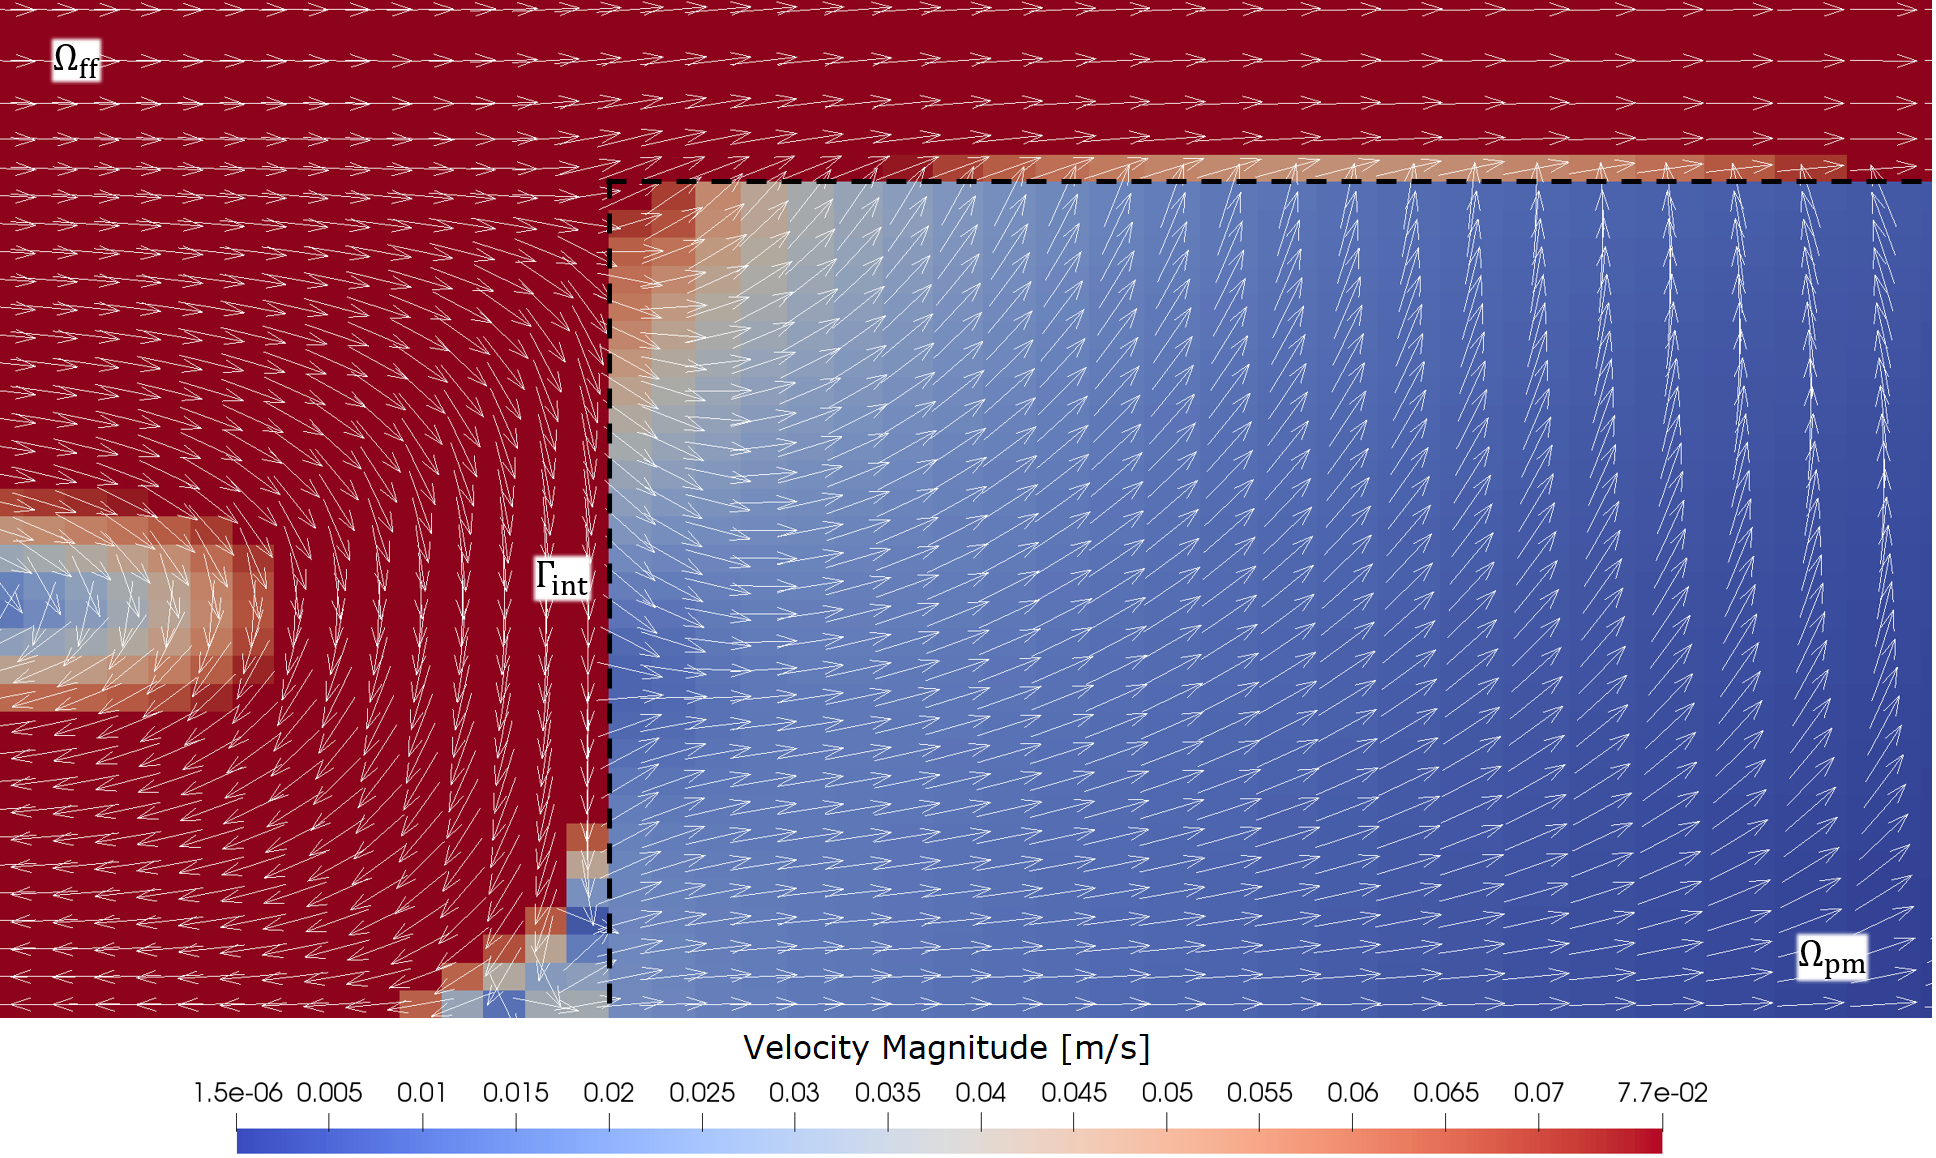
\includegraphics[height=0.8\textheight]{coupled_first_cavity_slides_labels.png}
	\caption{\tiny $\mathrm{K}=\SI{3.1e-7}{m^2}$, $Re=\num{6e5}$}
\end{figure}
\end{frame}
%%%%%%%%%%%%%%%%%%%%%%%%%%%%%%%%%%%%%%%%%%%%%%%%%%%%%%%%%%%%%%%%%%%%%%%%%%%
\begin{frame}{Coupled problem with shallow cavities}
\begin{figure}
	\centering
	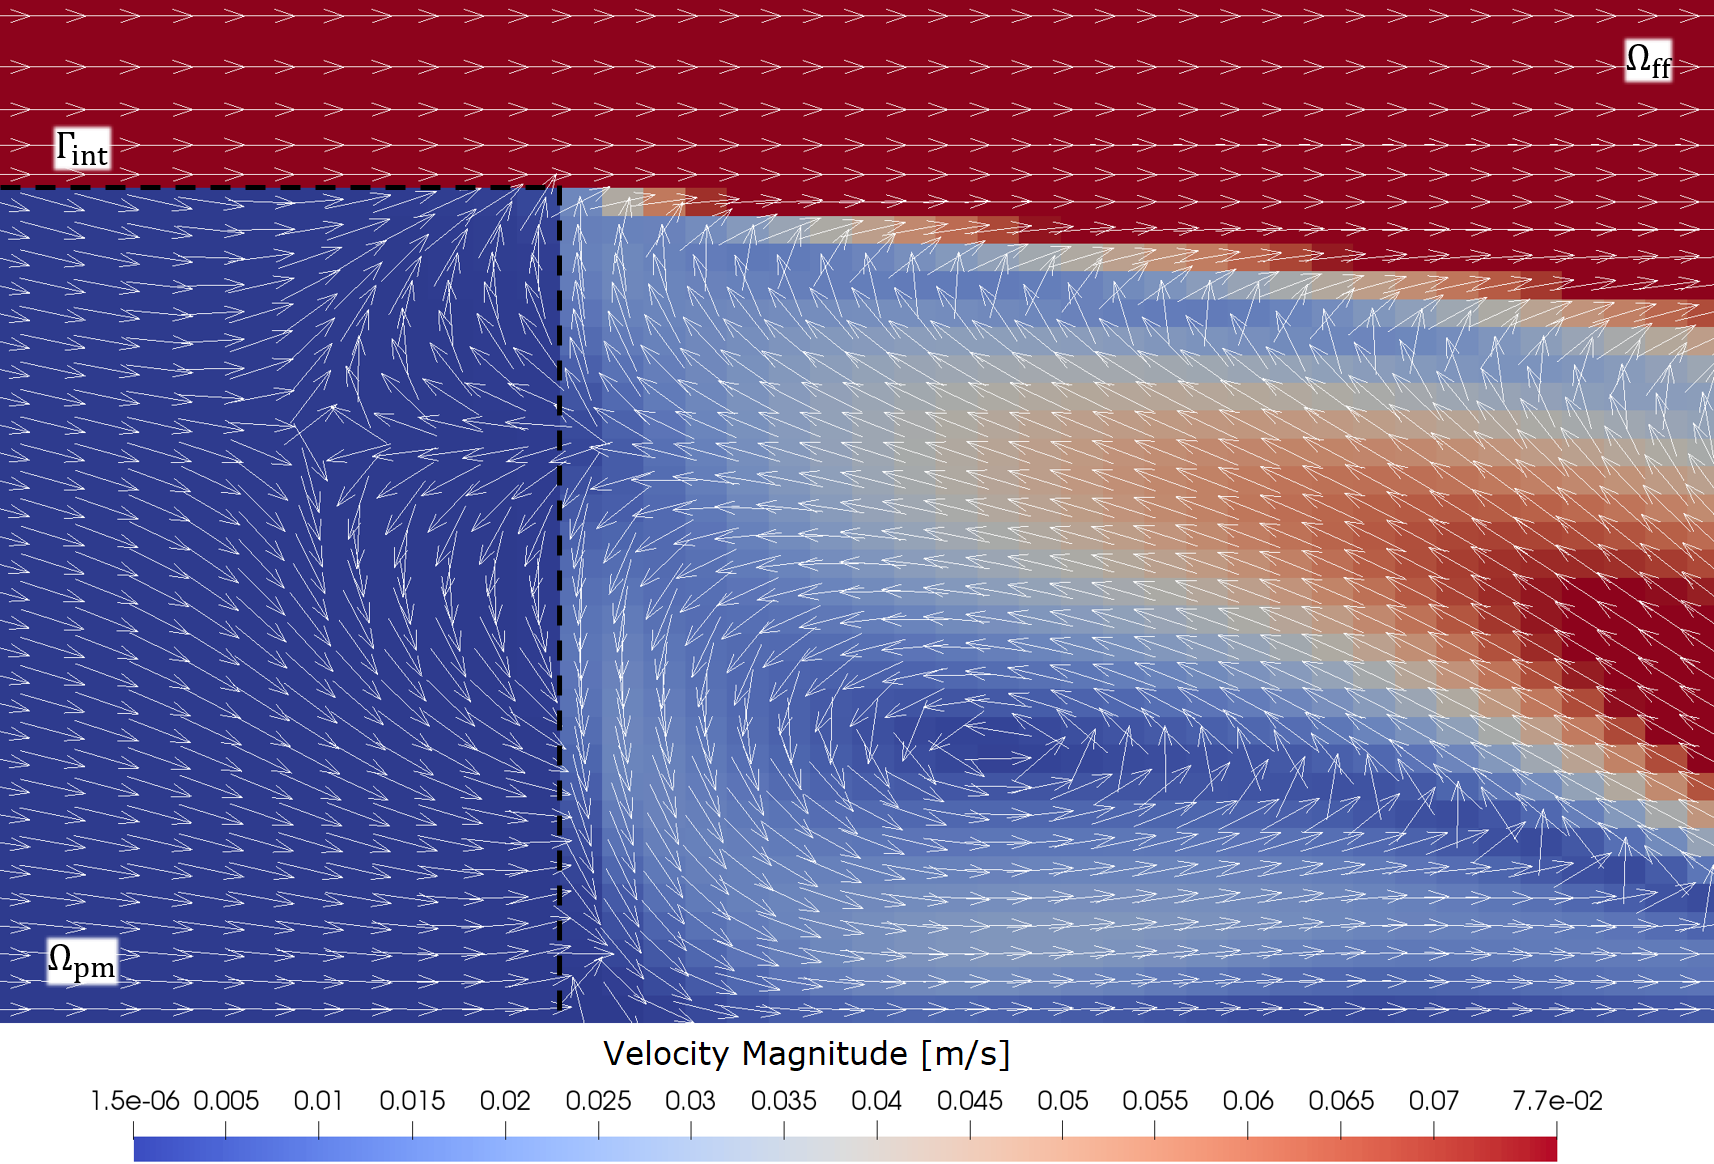
\includegraphics[height=0.82\textheight]{coupled_second_cavity_slides_labels.png}
	\caption{\tiny $\mathrm{K}=\SI{3.1e-7}{m^2}$, $Re=\num{6e5}$}
\end{figure}
\end{frame}
%%%%%%%%%%%%%%%%%%%%%%%%%%%%%%%
%\begin{frame}{Coupled problem with cavities}
%We change the domain considering deeper cavities ($\SI{0.3}{m}$ vs 
%$\SI{0.1}{m}$). We compute the \textbf{mass flow rate} from the free-flow 
%region to the porous-medium across $\Gamma_\text{int}$.
%\vspace{-1cm}
%\begin{columns}
%\column{0.5\textwidth}
%\begin{equation*}
%\dot{m} = \int_{\Gamma_\text{int}} \max \{ \varrho \mathbf{v} \cdot 
%\mathbf{n}_\text{ff} , 0 \} \; dA
%\end{equation*}
%\column{0.5\textwidth}
%\begin{figure}
%	\centering
%	% This file was created by matlab2tikz.
%
\definecolor{mycolor1}{rgb}{0.00000,0.44700,0.74100}%
\definecolor{mycolor2}{rgb}{0.85000,0.32500,0.09800}%

\begin{tikzpicture}

\begin{axis}[%
width=1.05\widthsette,
%width=0.951\widthsette,
height=0.95\widthsette,
at={(0\widthsette,0\widthsette)},
scale only axis,
xmode=log,
xmin=1e-12,
xmax=1e-05,
xlabel={$\mathrm{K} \; [\si{m^2}]$},
xlabel style={font=\scriptsize},
ymin=0.0005,
ymax=0.0045,
ylabel={$\dot{m} \; [\si{kg/s}]$},
ylabel style={font=\scriptsize},
axis background/.style={fill=white},
xmajorgrids,
ymajorgrids,
legend style={at={(0.03,0.97)}, anchor=north west, legend cell align=left, align=left, font=\tiny}
]
\addplot [color=mycolor1, line width=1.0pt, mark=o, mark options=solid]
  table[row sep=crcr]{%
3.1e-07	0.002690450574475\\
1.55e-07	0.00227104284972\\
3.1e-08	0.0013892852915599\\
3.1e-09	0.0007673545670522\\
3.1e-12	0.000648090673435001\\
};
\addlegendentry{Shallow cavities ($\SI{0.1}{m}$)}

\addplot [color=mycolor2, line width=1.0pt, mark=o, mark options=solid]
  table[row sep=crcr]{%
3.1e-07	0.00380516439666\\
1.55e-07	0.00306263879357\\
3.1e-08	0.001811656088526\\
3.1e-09	0.00108318452159\\
3.1e-12	0.000945936611289998\\
};
\addlegendentry{Deep cavities ($\SI{0.3}{m}$)}

\end{axis}
\end{tikzpicture}%
%\end{figure}
%\end{columns}
%\end{frame}
\begin{frame}{Coupled problem with cavities}
\textbf{Mass flow rate} $[\si{kg/s}]$ from the free-flow region to the porous-medium across $\Gamma_\text{int}$.
\begin{columns}
	\column{0.4\textwidth}
	\begin{equation*}
	\dot{m} = \int_{\Gamma_\text{int}} \max \{ \varrho \mathbf{v} \cdot 
	\mathbf{n}_\text{ff} , 0 \} \; dA
	\end{equation*}
	\column{0.6\textwidth}
	\begin{figure}
		\centering
		% This file was created by matlab2tikz.
%
\definecolor{mycolor1}{rgb}{0.00000,0.44700,0.74100}%
\definecolor{mycolor2}{rgb}{0.85000,0.32500,0.09800}%

\begin{tikzpicture}

\begin{axis}[%
width=1.05\widthsette,
%width=0.951\widthsette,
height=0.95\widthsette,
at={(0\widthsette,0\widthsette)},
scale only axis,
xmode=log,
xmin=1e-12,
xmax=1e-05,
xlabel={$\mathrm{K} \; [\si{m^2}]$},
xlabel style={font=\scriptsize},
ymin=0.0005,
ymax=0.0045,
ylabel={$\dot{m} \; [\si{kg/s}]$},
ylabel style={font=\scriptsize},
axis background/.style={fill=white},
xmajorgrids,
ymajorgrids,
legend style={at={(0.03,0.97)}, anchor=north west, legend cell align=left, align=left, font=\tiny}
]
\addplot [color=mycolor1, line width=1.0pt, mark=o, mark options=solid]
  table[row sep=crcr]{%
3.1e-07	0.002690450574475\\
1.55e-07	0.00227104284972\\
3.1e-08	0.0013892852915599\\
3.1e-09	0.0007673545670522\\
3.1e-12	0.000648090673435001\\
};
\addlegendentry{Shallow cavities ($\SI{0.1}{m}$)}

\addplot [color=mycolor2, line width=1.0pt, mark=o, mark options=solid]
  table[row sep=crcr]{%
3.1e-07	0.00380516439666\\
1.55e-07	0.00306263879357\\
3.1e-08	0.001811656088526\\
3.1e-09	0.00108318452159\\
3.1e-12	0.000945936611289998\\
};
\addlegendentry{Deep cavities ($\SI{0.3}{m}$)}

\end{axis}
\end{tikzpicture}%
	\end{figure}
\end{columns}
\end{frame}
%%%%%%%%%%%%%%%%%%%%%%%%%%%%%%%%%%%%%%%%%%%%%%%%%%%%%%%%%%%%%%%%%%%%%%%%%%%
\section{Conclusions}
\begin{frame}{Conclusions}
TVD methods:
\begin{itemize}
	\item \textbf{improved accuracy}.
	\item improved prediction of the reattachment length in the backward facing step test.
\end{itemize}
Free-flow and porous-medium flow coupling:
\begin{itemize}
	\item mutual influence of cavities.
	\item \textbf{permeability influence} on the flow field.
	\item mass flow rate.
\end{itemize}
\pause
Outlook:
\begin{itemize}
	\item other kinds of roughness.
	\item more \textbf{complex scenarios} (non-isothermal, multiphase, etc).
	\item high order methods on adapted grid with hanging nodes.
\end{itemize}
\end{frame}
%%%%%%%%%%%%%%%%%%%%%%%%%%%%%%%%%%%%%%%%%%%%%%%%%%%%%%%%%%%%%%%%%%%%%
\end{document}